% !TeX root = ../quantum.tex

\chapter{توزیع کلید کوانتومی}\label{chap:6}



\section{مبانی رمزنگاری}
\label{sec:6-1}


سیستم رمزنگاری\LTRfootnote{Cryptographic system} پایه مبتنی بر کلید در شکل \ref{fig:6-1} نشان داده شده است. منبع، پیام (متن‌آشکار\LTRfootnote{Plaintext}) $\bm{M}$ را به سمت بلوک رمزگذاری\LTRfootnote{Encryption} ارسال می‌کند که این بلوک با کمک کلید $\bm{K}$ دریافت شده از منبع کلید، رمزنگاشت\LTRfootnote{Cryptogram} را تولید می‌نماید. در سمت گیرنده، رمزنگاشت ارسال شده از طریق یک کانال ناامن، توسط الگوریتم رمزگشایی\LTRfootnote{Decryption} به همراه کلید $\bm{K}$ که از طریق کانال امن دریافت شده است، پردازش می‌شود که متن‌آشکار اصلی را برای تحویل به کاربر احرازهویت‌شده\LTRfootnote{Authenticated user} بازسازی می‌کند. فرآیند رمزگذاری را می‌توان به‌صورت ریاضی به‌صورت $E_{\bm{K}}(\bm{M}) = \bm{C}$ توصیف کرد، در حالی که فرآیند رمزگشایی با $D_{\bm{K}}(\bm{C}) = \bm{M}$ بیان می‌شود. ترکیب توابع رمزگشایی و رمزگذاری منجر به نگاشت همانی\LTRfootnote{Identity mapping} $D_{\bm{K}}(E_{\bm{K}}(\bm{M})) = \bm{M}$ می‌گردد. منبع کلید معمولاً کلید را به‌صورت تصادفی از فضای کلید\LTRfootnote{Keyspace} (محدوده تمام مقادیر ممکن برای کلید) تولید می‌کند.

الگوریتم‌های مبتنی بر کلید را می‌توان به دو دسته کلی تقسیم کرد:
\begin{itemize}
	\item در الگوریتم‌های متقارن\LTRfootnote{Symmetric algorithms}، کلید رمزگشایی را می‌توان از کلید رمزگذاری مشتق کرد و بالعکس. متناوباً، می‌توان از یک کلید یکسان برای هر دو مرحله رمزگذاری و رمزگشایی استفاده کرد. الگوریتم‌های متقارن با نام‌های الگوریتم‌های تک‌کلیدی\LTRfootnote{One-key (single-key) algorithms} یا کلید مخفی\LTRfootnote{Secret-key algorithms} نیز شناخته می‌شوند. یک سیستم شناخته‌شده که از این نوع الگوریتم استفاده می‌کند، استاندارد رمزگذاری دیجیتال\LTRfootnote{Digital encryption standard (DES)} است \cite{1,2,3,4}.
	\item در الگوریتم‌های نامتقارن\LTRfootnote{Asymmetric algorithms}، کلیدهای رمزگذاری و رمزگشایی متفاوت هستند. علاوه بر این، کلید رمزگشایی را نمی‌توان از روی کلید رمزگذاری تعیین کرد، حداقل نه در یک بازه زمانی معقول. به همین دلیل، کلیدهای رمزگذاری حتی می‌توانند به‌صورت عمومی منتشر شوند؛ زیرا یک شنودگر\LTRfootnote{Eavesdropper} قادر به تعیین کلید رمزگشایی نخواهد بود. سیستم‌های کلید عمومی\LTRfootnote{Public-key systems} \cite{5} بر پایه این مفهوم بنا شده‌اند. در سیستم‌های کلید عمومی، کلیدهای رمزگذاری عمومی می‌شوند، در حالی که کلید رمزگشایی تنها برای کاربر موردنظر شناخته شده است. در این حالت، کلید رمزگذاری را کلید عمومی\LTRfootnote{Public key} و کلید رمزگشایی را کلید مخفی (خصوصی)\LTRfootnote{Secret (private) key} می‌نامند. این کلیدها را می‌توان با هر ترتیبی برای ایجاد رمزنگاشت از متن‌آشکار و بازسازی متن‌آشکار از رمزنگاشت به کار برد.
\end{itemize}

\begin{figure}[h]
	\centering
	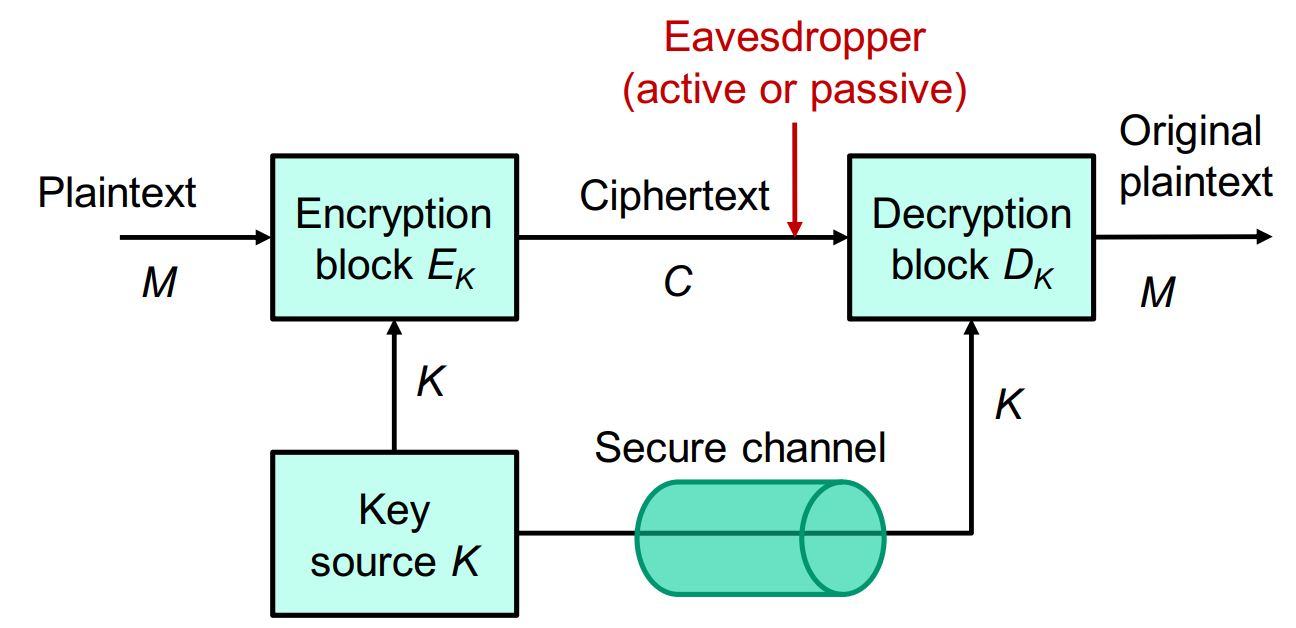
\includegraphics[width=0.7\linewidth]{chapters/figs/fig-6-1}
	\caption{طرح رمزنگاری پایه مبتنی بر کلید.}
	\label{fig:6-1}
\end{figure}

ساده‌ترین سیستم رمزنگاری کلید خصوصی، رمز ورنام\LTRfootnote{Vernam cipher} (پد یک‌بار مصرف\LTRfootnote{One-time pad}) است. در یک پد یک‌بار مصرف \cite{6}، یک دنباله کاملاً تصادفی از نویسه‌ها، با طولی برابر با طول دنباله پیام، به‌عنوان کلید استفاده می‌شود. برای هر پیام جدید، یک دنباله تصادفی دیگر به‌عنوان کلید به کار می‌رود و از این رو، طرح پد یک‌بار مصرف امنیت کامل\LTRfootnote{Perfect security} را فراهم می‌کند. به بیان دقیق‌تر، رویکرد جستجوی جامع\LTRfootnote{Brute-force search} مستلزم بررسی $m^n$ کلید احتمالی است که در آن $m$ اندازه الفبای به‌کار رفته و $n$ طول رمزنگاشتِ شنود شده است. در عمل، در ارتباطات دیجیتال و کامپیوتری، ما معمولاً در الفبای باینری $\mathrm{GF}(2) = \{0,1\}$ عمل می‌کنیم. برای به‌دست آوردن کلید، به یک مولد تصادفی خاص نیاز داریم و برای رمزگذاری با استفاده از طرح پد یک‌بار مصرف، صرفاً عمل جمع در پیمانه ۲، یعنی یک عملیات \lr{XOR}، را مطابق شکل \ref{fig:6-2} انجام می‌دهیم. طرح پد یک‌بار مصرف علی‌رغم ارائه امنیت کامل، چندین نقص دارد \cite{7,8,9}: این طرح مستلزم آن است که کلیدها به‌صورت امن توزیع شوند، طول آن‌ها حداقل به اندازه پیام باشد، بیت‌های کلید مجدداً استفاده نشوند، به‌صورت پیش‌تحویل ارائه شوند، تا زمان استفاده به‌صورت امن ذخیره گردند و پس از استفاده نابود شوند.

طبق گفته شانون \cite{10}، امنیت کامل که با نام امنیت غیرمشروط\LTRfootnote{Unconditional security} نیز شناخته می‌شود، زمانی حاصل می‌گردد که پیام‌های $\bm{M}$ و رمزنگاشت‌های $\bm{C}$ از نظر آماری مستقل باشند، به‌طوری که اطلاعات متقابل\LTRfootnote{Mutual information} متناظر با آن‌ها برابر صفر شود:
\begin{equation}
	I(\bm{M}; \bm{C}) = H(\bm{M}) - H(\bm{M}|\bm{C}) = 0 \implies H(\bm{M}|\bm{C}) = H(\bm{M})
	\label{eq:6-1}
\end{equation}
با به‌کارگیری قاعده زنجیره‌ای\LTRfootnote{Chain rule} \cite{2,11} که به‌صورت $H(X,Y) = H(X) + H(Y|X)$ بیان می‌شود، می‌توانیم بنویسیم:
\begin{equation}
	H(\bm{M}) = H(\bm{M}|\bm{C}) \leq H(\bm{M}, \bm{K}|\bm{C}) = H(\bm{K}|\bm{C}) + \underbrace{H(\bm{M}|\bm{C}, \bm{K})}_{=0} \leq H(\bm{K})
	\label{eq:6-2a}
\end{equation}
که در آن از این واقعیت استفاده شده است که وقتی هم رمزنگاشت و هم کلید معلوم باشند، پیام کاملاً مشخص می‌شود؛ یعنی $H(\bm{M}|\bm{K}, \bm{C}) = 0$. بنابراین، شرط امنیت کامل را می‌توان به‌صورت زیر خلاصه کرد:
\begin{equation}
	H(\bm{M}) \leq H(\bm{K})
	\label{eq:6-2b}
\end{equation}
به عبارت دیگر، برای اینکه یک طرح رمزگذاری دارای امنیت کامل باشد، آنتروپی\LTRfootnote{Entropy} (عدم قطعیت\LTRfootnote{Uncertainty}) کلید نمی‌تواند کمتر از آنتروپی پیام باشد. با توجه به اینکه طول کلید در رمز ورنام حداقل برابر با طول پیام است، به نظر می‌رسد طرح پد یک‌بار مصرف دارای امنیت کامل باشد.

\begin{figure}[H]
	\centering
	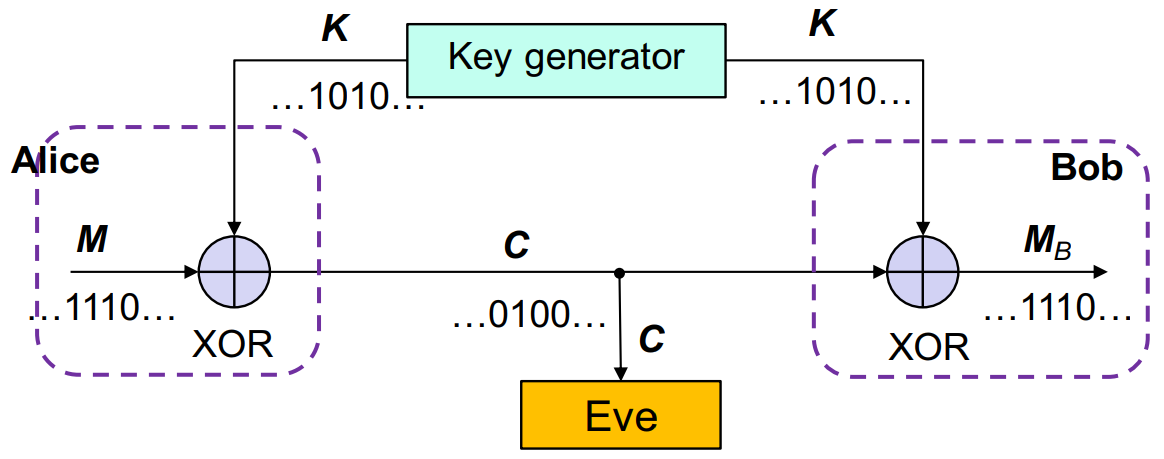
\includegraphics[width=0.7\linewidth]{chapters/figs/fig-6-2}
	\caption{طرح رمزگذاری پد یک‌بار مصرف.}
	\label{fig:6-2}
\end{figure}




\section{مبانی توزیع کلید کوانتومی}
\label{sec:6-2}

اخیراً دستاوردهای قابل‌توجهی در محاسبات کوانتومی حاصل شده است \cite{7,8,9}. بسیاری از شرکت‌ها در حال حاضر مشغول توسعه کامپیوترهای کوانتومی با مقیاس متوسط هستند. از آنجایی که اکثر سیستم‌های رمزنگاری به فرض دشواری محاسباتی\LTRfootnote{Computational hardness assumption} وابسته هستند، محاسبات کوانتومی چالشی جدی برای سیستم‌های امنیت سایبری مدرن محسوب می‌شود. به‌عنوان مثال، برای شکستن پروتکل ریواست-شامیر-ادلمن (\lr{RSA})\LTRfootnote{Rivest-Shamir-Adleman (RSA)} \cite{20}، باید دوره تناوب $r$ تابع $f(x) = m^x \pmod n = f(x+r)$ را تعیین کرد (به‌طوری که $r = 0, 1, \dots, 2^{L-1}$ و $m$ یک عدد صحیح کوچک‌تر از $n-1$ است). این دوره تناوب در یک مرحله از الگوریتم تجزیه شور \cite{7,8,9,17,18,19} تعیین می‌شود.

توزیع کلید کوانتومی (\lr{QKD}) با رمزگذاری متقارت را می‌توان به‌عنوان یک طرح امنیت لایه فیزیکی\LTRfootnote{Physical-layer security} تفسیر کرد که امنیت اثبات‌پذیری را در برابر حملات آغاز شده توسط کامپیوترهای کوانتومی فراهم می‌کند \cite{21}. اولین طرح \lr{QKD} توسط بنت\LTRfootnote{Bennett} و براسارد\LTRfootnote{Brassard} معرفی شد که آن را در سال ۱۹۸۴ پیشنهاد کردند \cite{15,16} و امروزه با نام پروتکل \lr{BB84} شناخته می‌شود. امنیت \lr{QKD} توسط قوانین مکانیک کوانتومی تضمین می‌شود. درجات آزادی فوتون\LTRfootnote{Degree-of-freedom (DOF)} (\lr{DOF}) مختلفی مانند قطبش\LTRfootnote{Polarization}، زمان، فرکانس، فاز و تکانه زاویه‌ای مداری\LTRfootnote{Orbital angular momentum} را می‌توان برای پیاده‌سازی پروتکل‌های مختلف \lr{QKD} به کار گرفت. به‌طور کلی، بسته به استراتژی اعمال شده در سمت باب\LTRfootnote{Bob}، دو طرح کلی \lr{QKD} وجود دارد: \lr{QKD} با متغیر گسسته\LTRfootnote{Discrete-variable QKD (DV-QKD)} (\lr{DV-QKD}) و \lr{QKD} با متغیر پیوسته\LTRfootnote{Continuous-variable QKD (CV-QKD)} (\lr{CV-QKD}). در طرح‌های \lr{DV-QKD}، یک آشکارساز تک‌فوتون\LTRfootnote{Single-photon detector (SPD)} (\lr{SPD}) در سمت باب به کار می‌رود، در حالی که در \lr{CV-QKD}، مولفه‌های مربعی میدان\LTRfootnote{Field quadratures} با کمک آشکارسازی هموداین/هتروداین\LTRfootnote{Homodyne/heterodyne detection} اندازه‌گیری می‌شوند. طرح \lr{DV-QKD} با به‌کارگیری قضیه کپی‌ناپذیری\LTRfootnote{No-cloning theorem} و قضیه تمایزناپذیری حالت‌های کوانتومی دلخواه\LTRfootnote{Indistinguishability of arbitrary quantum states} به امنیت غیرمشروط دست می‌یابد. قضیه کپی‌ناپذیری ادعا می‌کند که حالت‌های کوانتومی دلخواه را نمی‌توان کپی کرد، که نشان می‌دهد ایو\LTRfootnote{Eve} نمی‌تواند حالت‌های کوانتومی غیرمتعامد\LTRfootnote{Nonorthogonal} را حتی با کمک یک کامپیوتر کوانتومی بازتولید کند. از سوی دیگر، قضیه دوم بیان می‌کند که حالت‌های غیرمتعامد را نمی‌توان به‌طور ابهام‌ناپذیر متمایز کرد. به عبارت دیگر، هنگامی که ایو با حالت‌های کوانتومی ارسال‌شده تعامل برقرار می‌کند تا اطلاعاتی درباره بیت‌های ارسالی به‌دست آورد، به‌طور ناخواسته وفاداری\LTRfootnote{Fidelity} حالت‌های کوانتومی را مختل می‌کند که باب آن را آشکار خواهد کرد. از طرف دیگر، \lr{CV-QKD} از اصل عدم قطعیت\LTRfootnote{Uncertainty principle} بهره می‌برد که بیان می‌کند هر دو مولفه هم‌فاز\LTRfootnote{In-phase} و مربعی\LTRfootnote{Quadrature} حالت‌های همدوس\LTRfootnote{Coherent states} را نمی‌توان به‌طور هم‌زمان با دقت کامل اندازه‌گیری کرد. ما همچنین می‌توانیم طرح‌های مختلف \lr{QKD} را به دو نوع «به کمک درهم‌تنیدگی»\LTRfootnote{Entanglement-assisted} یا «آماده‌سازی-و-اندازه‌گیری»\LTRfootnote{Prepare-and-measure} طبقه‌بندی کنیم.

\begin{figure}[H]
	\centering
	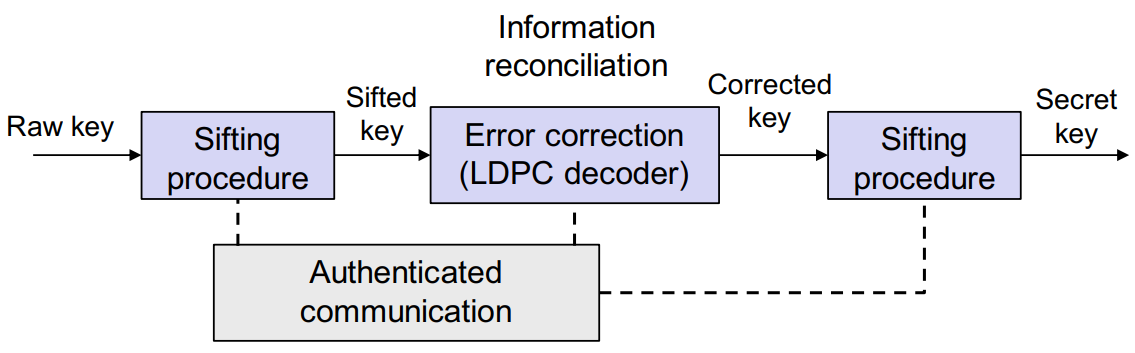
\includegraphics[width=0.9\linewidth]{chapters/figs/fig-6-3}
	\caption{مراحل پس‌پردازش کلاسیک.}
	\label{fig:6-3}
\end{figure}

مصالحه اطلاعات چیزی جز تصحیح خطا نیست که بر روی یک کانال عمومی\LTRfootnote{Public channel} انجام می‌شود و خطاها را بین $\bm{X}$ و $\bm{Y}$ مصالحه می‌کند تا یک رشته بیت مشترک $\bm{K}$ به‌دست آید، در حالی که اطلاعات فاش‌شده برای ایو تا حد امکان کمینه باشد.

تقویت حریم خصوصی\LTRfootnote{Privacy amplification} \cite{23, 24} بین آلیس و باب برای استخراج\LTRfootnote{Distill} مجموعه کوچکتری از بیت‌ها $\bm{S}$ از $\bm{K}$ استفاده می‌شود که همبستگی آن با رشته ایو $\bm{Z}$ زیر آستانه مطلوب باشد. یکی از راه‌های انجام تقویت حریم خصوصی، استفاده از توابع هش سراسری\LTRfootnote{Universal hash functions} $G$ است که مجموعه رشته‌های $n$-بیتی $A$ را به مجموعه رشته‌های $m$-بیتی $B$ نگاشت می‌کنند، به‌طوری که برای هر دو رشته متمایز $a_1, a_2 \in A$، وقتی $g$ به‌صورت یکنواخت و تصادفی از $G$ انتخاب شود، احتمال برقراری $g(a_1) = g(a_2)$ حداکثر $1/|B|$ باشد.

جزئیات بیشتر در مورد مصالحه اطلاعات و تقویت حریم خصوصی در بخش \ref{sec:6-9} از این فصل ارائه خواهد شد.





\section{قضیه کپی‌ناپذیری و تمایز حالت‌های کوانتومی}
\label{sec:6-3}

\begin{theorem}
	\label{thm:6-1}
	\textbf{(قضیه کپی‌ناپذیری\LTRfootnote{No-cloning theorem})}
	هیچ کپی‌کننده کوانتومی وجود ندارد که بتواند یک حالت کوانتومی دلخواه را کپی کند.
\end{theorem}

\begin{proof}
	اگر حالت ورودی $|\psi\rangle$ باشد، خروجی کپی‌کننده باید به صورت $|\psi\rangle|\psi\rangle$ باشد. برای یک حالت کوانتومی دلخواه، وجود چنین کپی‌کننده‌ای منجر به یک تناقض بنیادی می‌شود. دو حالت دلخواه $|\psi\rangle$ و $|\phi\rangle$ را در نظر بگیرید که به عنوان ورودی به کپی‌کننده داده می‌شوند. وقتی این حالت‌ها به صورت مجزا وارد شوند، انتظار داریم خروجی‌های $|\psi\rangle|\psi\rangle$ و $|\phi\rangle|\phi\rangle$ را به‌دست آوریم. اکنون برهم‌نهی\LTRfootnote{Superposition} این دو حالت را به صورت زیر در نظر بگیرید:
	\begin{equation}
		\begin{aligned}
			|\Psi\rangle = a|\psi\rangle + b|\phi\rangle \implies |\Psi\rangle|\Psi\rangle &= (a|\psi\rangle + b|\phi\rangle)(a|\psi\rangle + b|\phi\rangle) \\ &= a^2|\psi\rangle|\psi\rangle + ab|\psi\rangle|\phi\rangle + ab|\phi\rangle|\psi\rangle + b^2|\phi\rangle|\phi\rangle
		\end{aligned}
		\label{eq:6-3}
	\end{equation}
	از سوی دیگر، خطی بودن مکانیک کوانتومی به ما می‌گوید که کپی‌کننده کوانتومی را می‌توان با یک عملگر یکانی\LTRfootnote{Unitary operator} بازنمایی کرد که عمل کپی کردن را انجام می‌دهد. اگر چنین عملگر یکانی بر روی حالت برهم‌نهی $|\Psi\rangle$ اثر کند، خروجی باید برهم‌نهی از $|\psi\rangle|\psi\rangle$ و $|\phi\rangle|\phi\rangle$ باشد؛ یعنی:
	\begin{equation}
		|\Psi'\rangle = a|\psi\rangle|\psi\rangle + b|\phi\rangle|\phi\rangle
		\label{eq:6-4}
	\end{equation}
	تفاوت بین دو معادله \eqref{eq:6-3} و \eqref{eq:6-4} منجر به تناقض ذکر شده در بالا می‌شود. در نتیجه، هیچ عملگر یکانی وجود ندارد که بتواند $|\Psi\rangle$ را کپی کند.
\end{proof}

این نتیجه پرسش مرتبطی را ایجاد می‌کند: آیا حالت‌های خاصی وجود دارند که کپی کردن آن‌ها امکان‌پذیر باشد؟ پاسخ به این پرسش (به‌طور شگفت‌انگیزی) مثبت است؛ کپی کردن تنها برای حالت‌های متعامد متقابل امکان‌پذیر است.

\begin{theorem}
	\label{thm:6-2}
	تمایز ابهام‌ناپذیر حالت‌های کوانتومی غیرمتعامد غیرممکن است.
	
	
	به عبارت دیگر، هیچ دستگاه اندازه‌گیری نمی‌توان ساخت که بتواند با اطمینان حالت‌های غیرمتعامد را متمایز کند. این نتیجه بنیادی نقش مهمی در رمزنگاری کوانتومی ایفا می‌کند.
\end{theorem}

\begin{proof}
	اثبات این قضیه بر پایه تناقض\LTRfootnote{Contradiction} است. فرض کنید عملگر اندازه‌گیری $M$ یک عملگر هرمیتی\LTRfootnote{Hermitian operator} با مقادیر ویژه\LTRfootnote{Eigenvalues} $m_i$ و عملگرهای تصویر\LTRfootnote{Projection operators} $P_i$ متناظر باشد که به ما اجازه می‌دهد به‌طور ابهام‌ناپذیر بین دو حالت غیرمتعامد $|\psi_1\rangle$ و $|\psi_2\rangle$ تمایز قائل شویم. مقدار ویژه $m_1$ ($m_2$) به‌طور ابهام‌ناپذیر حالت $|\psi_1\rangle$ ($|\psi_2\rangle$) را شناسایی می‌کند. می‌دانیم که برای عملگرهای تصویر، ویژگی‌های زیر برقرار است:
	\begin{equation}
		\langle\psi_1|P_1|\psi_1\rangle = 1; \quad \langle\psi_2|P_2|\psi_2\rangle = 1; \quad \langle\psi_1|P_2|\psi_1\rangle = 0; \quad \langle\psi_2|P_1|\psi_2\rangle = 0
		\label{eq:6-5}
	\end{equation}
	با توجه به موارد فوق، $|\psi_2\rangle$ را می‌توان برحسب $|\psi_1\rangle$ و حالت دیگری مانند $|\phi\rangle$ که بر $|\psi_1\rangle$ متعامد است، به صورت زیر نمایش داد:
	\begin{equation}
		|\psi_2\rangle = a|\psi_1\rangle + b|\phi\rangle
		\label{eq:6-6}
	\end{equation}
	برای برقراری رابطه \eqref{eq:6-5}، $|\psi_2\rangle$ باید با $|\phi\rangle$ برابر باشد (یعنی $a=0$)، که این امر نشان‌دهنده یک تناقض است (زیرا فرض شده بود دو حالت غیرمتعامد هستند).
\end{proof}





\section{پروتکل‌های توزیع کلید کوانتومی با متغیر گسسته}
\label{sec:6-4}

در این بخش، برخی از پروتکل‌های مرتبط با \lr{DV-QKD} از جمله \lr{BB84}، \lr{B92}، کدگذاری فاز-زمان\LTRfootnote{Time-phase encoding}، \lr{E91} و پروتکل‌های اینشتین-پودولسکی-روزن (\lr{EPR})\LTRfootnote{Einstein-Podolsky-Rosen (EPR)} را شرح می‌دهیم.

\subsection{پروتکل‌های \lr{BB84}}
\label{subsec:6-4-1}

پروتکل \lr{BB84} به نام بنت\LTRfootnote{Bennett} و براسارد\LTRfootnote{Brassard} نام‌گذاری شده است که آن را در سال ۱۹۸۴ پیشنهاد کردند \cite{15,16}. سه اصل کلیدی به‌کار گرفته شده در این پروتکل عبارتند از: قضیه کپی‌ناپذیری، فروپاشی حالت\LTRfootnote{State collapse} در طول اندازه‌گیری، و بازگشت‌ناپذیری اندازه‌گیری‌ها\LTRfootnote{Irreversibility of measurements} \cite{7}. پروتکل \lr{BB84} را می‌توان با استفاده از درجات آزادی مختلف، از جمله درجه آزادی قطبش\LTRfootnote{Polarization} \cite{25} یا فاز فوتون‌ها \cite{22} پیاده‌سازی کرد. از نظر تجربی، پروتکل \lr{BB84} در هر دو کانال فیبر نوری و نوری فضای آزاد (\lr{FSO})\LTRfootnote{Free-space-optical (FSO)} نمایش داده شده است \cite{25,26}. پروتکل \lr{BB84} مبتنی بر قطبش در کانال‌های فیبر نوری تحت تأثیر پاشندگی مد قطبشی\LTRfootnote{Polarization mode dispersion}، تلفات وابسته به قطبش\LTRfootnote{Polarization-dependent loss} و تلفات فیبر قرار می‌گیرد که مسافت ارسال را محدود می‌کنند. برای افزایش مسافت ارسال، از کدگذاری فاز استفاده می‌شود، مانند آنچه در مرجع \cite{26} آمده است. متأسفانه نرخ کلید امن در ۴۰۵ کیلومتر فیبر با تلفات بسیار کم، بسیار ناچیز و تنها برابر با $6.5$ بیت بر ثانیه است. در یک کانال \lr{FSO}، اثرات قطبش به حداقل می‌رسد؛ با این حال، تلاطم اتمسفری\LTRfootnote{Atmospheric turbulence} می‌تواند منجر به اعوجاج جبهه‌موج\LTRfootnote{Wavefront distortion} و نوسانات فاز تصادفی شود. نمایش‌های قبلی \lr{QKD} شامل پیوند \lr{FSO} ماهواره به زمین و پیوند \lr{FSO} بین دو نقطه در جزایر قناری بوده است \cite{25}.

دو پایه‌ای که در پروتکل \lr{BB84} استفاده می‌شوند، پایه محاسباتی\LTRfootnote{Computational basis} $CB = \{|0\rangle, |1\rangle\}$ و پایه قطری\LTRfootnote{Diagonal basis} هستند:
\begin{equation}
	DB = \left\{ |+\rangle = \frac{|0\rangle + |1\rangle}{\sqrt{2}} ; \quad |-\rangle = \frac{|0\rangle - |1\rangle}{\sqrt{2}} \right\}
	\label{eq:6-7}
\end{equation}
این پایه‌ها به دسته‌ای از پایه‌های متقابلاً بدون سوگیری\LTRfootnote{Mutually unbiased bases (MUBs)} (\lr{MUBs}) تعلق دارند \cite{27,28,29,30,31}. دو پایه متعامد\LTRfootnote{Orthonormal bases} $\{|e_1\rangle, \dots, |e_N\rangle\}$ و $\{|f_1\rangle, \dots, |f_N\rangle\}$ در فضای هیلبرت $\mathbb{C}^N$ زمانی \lr{MUB} هستند که مجذور اندازه ضرب داخلی بین هر دو حالت پایه $\{|e_m\rangle\}$ و $\{|f_n\rangle\}$ برابر با معکوس بعد باشد:
\begin{equation}
	|\langle e_m | f_n \rangle|^2 = \frac{1}{N} \quad m, n \in \{1, \dots, N\}
	\label{eq:6-8}
\end{equation}
واژه کلیدی «بدون سوگیری»\LTRfootnote{Unbiased} بدین معناست که اگر سیستمی در حالتی متعلق به یکی از پایه‌ها آماده‌سازی شود، تمام نتایج اندازه‌گیری نسبت به پایه‌های دیگر به یک اندازه محتمل هستند.

آلیس به‌طور تصادفی یک \lr{MUB} و به دنبال آن به‌طور تصادفی یک حالت پایه را انتخاب می‌کند. مقدار منطقی $0$ توسط حالت‌های $|0\rangle$ و $|+\rangle$، و مقدار منطقی $1$ توسط $|1\rangle$ و $|-\rangle$ بازنمایی می‌شود. باب هر کیوبیت را با انتخاب تصادفی پایه (محاسباتی یا قطری) اندازه‌گیری می‌کند. در یک فرآیند غربال‌گری\LTRfootnote{Sifting procedure}، آلیس و باب پایه‌های استفاده شده برای هر کیوبیت را اعلام کرده و تنها مواردی را نگه می‌دارند که در آن‌ها از پایه یکسانی استفاده شده است.

اکنون پروتکل \lr{QKD} مبتنی بر قطبش \lr{BB84} را با چهار حالت متناظر به‌کار رفته، مطابق شکل \ref{fig:6-4} شرح می‌دهیم. پیاده‌سازی با قطعات اپتیکی حجیم\LTRfootnote{Bulky optics} برای پروتکل \lr{BB84} در شکل \ref{fig:6-5} تصویر شده است.

حالت خروجی لیزر با عنوان حالت همدوس\LTRfootnote{Coherent state} شناخته می‌شود \cite{31,32,33,34,35,36} که نشان‌دهنده کِت ویژه راست عملگر نابودی\LTRfootnote{Annihilation operator} $a$ است؛ یعنی $a|\alpha\rangle = \alpha|\alpha\rangle$ که در آن $\alpha$ مقدار ویژه مختلط است. بردار حالت همدوس $|\alpha\rangle$ را می‌توان برحسب کِت‌های ویژه متعامد $|n\rangle$ (حالت تعداد یا حالت فوک\LTRfootnote{Fock state}) عملگر تعداد $N = a^\dagger a$ به‌صورت زیر نشان داد:
\begin{equation}
	|\alpha\rangle = \exp\big(-\frac{|\alpha|^2}{2}\big) \sum_{n=0}^{\infty} \frac{\alpha^n}{\sqrt{n!}} |n\rangle
	\label{eq:6-9}
\end{equation}

\begin{figure}[H]
	\centering
	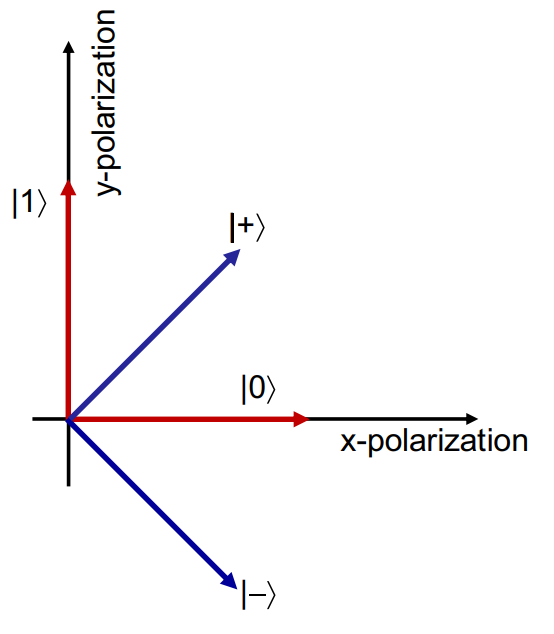
\includegraphics[width=0.5\linewidth]{chapters/figs/fig-6-4}
	\caption{چهار حالت به‌کار رفته در پروتکل \lr{BB84}.}
	\label{fig:6-4}
\end{figure}


حالت‌های همدوس متعامد نیستند، زیرا رابطه زیر برقرار است:
\begin{equation}
	\begin{aligned}
		|\langle\alpha | \beta\rangle|^2 &= \left| e^{-(|\alpha|^2+|\beta|^2)/2} \sum_{n=0}^{+\infty} \sum_{m=0}^{+\infty} (n!)^{-1/2}(m!)^{-1/2} \alpha^n (\beta^*)^m \langle n|m\rangle \right|^2 \\
		&= \left| e^{-(|\alpha|^2+|\beta|^2)/2} \sum_{n=0}^{+\infty} (n!)^{-1} \alpha^n (\beta^*)^n \right|^2 = \left| e^{-(|\alpha|^2+|\beta|^2-2\alpha\beta^*)/2} \right|^2 = e^{-|\alpha-\beta|^2}
	\end{aligned}
	\label{eq:6-10}
\end{equation}
با تضعیف کافی حالت همدوس، به حالت همدوس ضعیف\LTRfootnote{Weak coherent state (WCS)} (\lr{WCS}) دست می‌یابیم که در آن احتمال تولید بیش از یک فوتون بسیار کم است. برای مثال، به ازای $\alpha = 0.1$ خواهیم داشت:
$|0.1\rangle = \sqrt{0.90} |0\rangle + \sqrt{0.09} |1\rangle + \sqrt{0.002} |2\rangle + \dots$.
حالت تعداد $|n\rangle$ را می‌توان برحسب حالت پایه\LTRfootnote{Ground state} ($|0\rangle$) و با کمک عملگر تولید\LTRfootnote{Creation operator} به‌صورت زیر بیان کرد:


\begin{figure}[H]
	\centering
	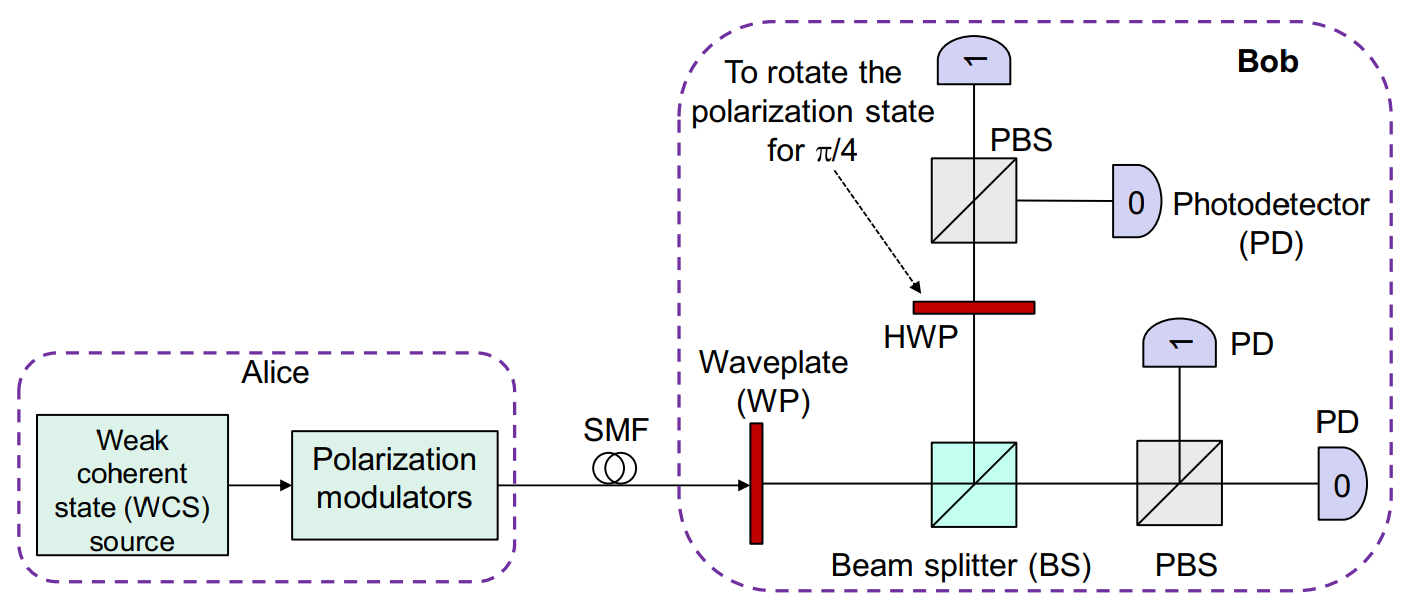
\includegraphics[width=\linewidth]{chapters/figs/fig-6-5}
	\caption{پروتکل \lr{BB84} مبتنی بر قطبش.}
	\label{fig:6-5}
\end{figure}




\begin{equation}
	|n\rangle = \frac{(a^\dagger)^n}{(n!)^{1/2}} |0\rangle 
	\label{eq:6-11}
\end{equation}
عملگر چگالی\LTRfootnote{Density operator} یک حالت همدوس به‌صورت زیر داده می‌شود:
\begin{equation}
	\rho = |\alpha\rangle\langle\alpha| = e^{-|\alpha|^2} \sum_{n=0}^{+\infty} \sum_{m=0}^{+\infty} \frac{\alpha^n (\alpha^*)^m}{(n!)^{1/2}(m!)^{1/2}} |n\rangle\langle m| 
	\label{eq:6-12}
\end{equation}
جملات قطری $\rho$ به‌صورت زیر تعیین می‌شوند:
\begin{equation}
	\langle n|\rho|n\rangle = e^{-|\alpha|^2} \frac{|\alpha|^{2n}}{n!} 
	\label{eq:6-13}
\end{equation}
که آشکارا یک توزیع پواسون\LTRfootnote{Poisson distribution} برای میانگین تعداد فوتون‌های $|\alpha|^2$ است. بنابراین، احتمال اینکه $n$ فوتون در یک حالت همدوس $|\alpha\rangle$ یافت شود، از توزیع پواسون پیروی می‌کند:
\begin{equation}
	P(n) = |\langle n|\alpha\rangle|^2 = \frac{e^{-\mu} \mu^n}{n!}
	\label{eq:6-14}
\end{equation}
که در آن از $\mu = |\alpha|^2$ برای نشان دادن میانگین تعداد فوتون‌ها استفاده می‌کنیم.

با توجه به اینکه اکنون احتمال ارسال چندین فوتون غیرصفر است، ایو می‌تواند از این واقعیت برای کسب اطلاعات از کانال بهره‌برداری کند که این کار با عنوان حمله تقسیم تعداد فوتون\LTRfootnote{Photon number splitting (PNS) attack} (\lr{PNS}) شناخته می‌شود. با فرض اینکه او بتواند تعداد فوتون‌هایی را که به او می‌رسد بدون انجام اندازه‌گیری روی سیستم تشخیص دهد، زمانی که چندین فوتون شناسایی شوند، ایو یک تک‌فوتون را برداشته و آن را در حافظه کوانتومی\LTRfootnote{Quantum memory} قرار می‌دهد تا زمانی که آلیس و باب غربال‌گری زمانی و مصالحه پایه‌ها را انجام دهند. با یادگیری پایه‌های اندازه‌گیری آلیس و باب از طریق بحث در کانال عمومی احرازهویت‌شده، فوتون‌های ذخیره‌شده در حافظه کوانتومی در پایه صحیح اندازه‌گیری می‌شوند و تمام اطلاعات موجود در فوتون را در اختیار ایو قرار می‌دهند.

برای غلبه بر حمله \lr{PNS}، استفاده از \lr{QKD} مبتنی بر حالت فریب\LTRfootnote{Decoy-state} در مرجع \cite{37} پیشنهاد شد. در \lr{QKD} حالت فریب، میانگین تعداد فوتون‌های ارسالی در بازه‌های زمانی تصادفی افزایش می‌یابد که به آلیس و باب اجازه می‌دهد تشخیص دهند که آیا در زمان ارسال چندین فوتون، ایو در حال سرقت فوتون‌ها است یا خیر.







\subsection{پروتکل B92}
\label{subsec:6-4-2}

پروتکل \lr{B92} که در سال $1992$ توسط بنت\LTRfootnote{Bennett} معرفی شد \cite{38}، تنها از دو حالت غیرمتعامد استفاده می‌کند که در شکل \ref{fig:6-6} نشان داده شده است. آلیس به‌طور تصادفی یک بیت کلاسیک $d$ تولید می‌کند و بسته به مقدار آن ($0$ یا $1$)، حالت زیر را برای باب ارسال می‌نماید \cite{7}:



\begin{figure}[ht]
	\centering
	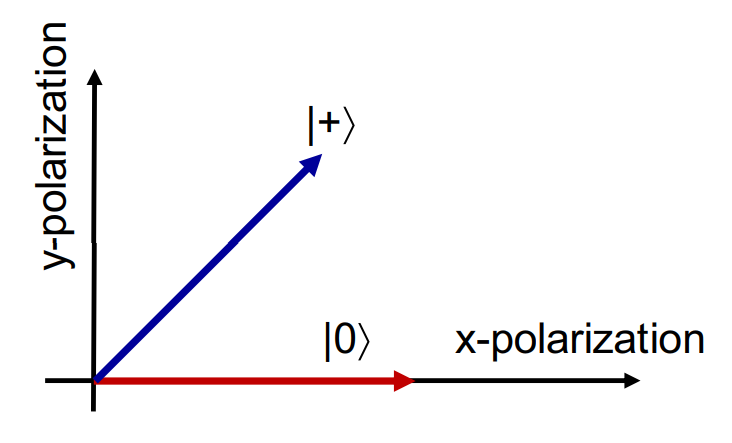
\includegraphics[width=0.6\textwidth]{chapters/figs/fig-6-6}
	\caption{دو حالت به‌کار رفته در پروتکل \lr{B92}.}
	\label{fig:6-6}
\end{figure}

\begin{equation}
	|\psi\rangle = 
	\begin{cases} 
		|0\rangle, & d = 0 \\ 
		|+\rangle = (|0\rangle + |1\rangle)/\sqrt{2}, & d = 1 
	\end{cases}
	\label{eq:6-15}
\end{equation}

باب به‌طور تصادفی یک بیت کلاسیک $d'$ تولید کرده و متعاقباً کیوبیت‌های دریافتی را در پایه $CB = \{|0\rangle, |1\rangle\}$ (اگر $d'=0$) یا در پایه $DB = \{|+\rangle, |-\rangle\}$ (اگر $d'=1$) اندازه‌گیری می‌کند؛ به‌طوری که نتیجه اندازه‌گیری $r=0$ یا $1$ متناظر با حالت‌های ویژه\LTRfootnote{Eigenstates} $1$ و $1+$ از مشاهده‌پذیرهای\LTRfootnote{Observables} $Z$ و $X$ است، همان‌طور که در جدول \ref{tab:6-1} نشان داده شده است. به‌وضوح، هنگامی که نتیجه اندازه‌گیری $r=0$ باشد، حالت‌های احتمالی ارسال شده توسط آلیس $|0\rangle$ و $|+\rangle$ هستند و باب نمی‌داند آلیس کدام حالت را ارسال کرده است. از سوی دیگر، وقتی نتیجه اندازه‌گیری $r=1$ باشد، حالت‌های احتمالی آشکار شده توسط باب $|1\rangle$ و $|-\rangle$ هستند و بیت آشکار شده توسط باب متمم بیت آلیس است. باب به‌صورت عمومی مقدار $r$ را اعلام می‌کند (و البته $d'$ را مخفی نگه می‌دارد). آلیس و باب تنها آن جفت‌های $\{d, d'\}$ را نگه می‌دارند که برای آن‌ها نتیجه اندازه‌گیری $r=1$ بوده است. بیت نهایی کلید برای آلیس $d$ و برای باب $1-d'$ است. پس از آن، مراحل مصالحه اطلاعات و تقویت حریم خصوصی انجام می‌شوند.




\subsection{پروتکل‌های اکرت (\lr{E91}) و اینشتین-پودولسکی-روزن}
\label{subsec:6-4-3}

پروتکل اکرت (\lr{E91})\LTRfootnote{Ekert (E91) protocol} توسط اکرت در سال ۱۹۹۱ معرفی شد \cite{39} (همچنین ببینید \cite{7}). فرض کنید آلیس و باب $n$ جفت کیوبیت درهم‌تنیده\LTRfootnote{Entangled pairs} در حالت بل\LTRfootnote{Bell state} (جفت \lr{EPR}\LTRfootnote{Einstein-Podolsky-Rosen (EPR)}) $|B_{00}\rangle$ به اشتراک می‌گذارند:
\begin{equation}
	|B_{00}\rangle = \frac{|00\rangle + |11\rangle}{\sqrt{2}}
	\label{eq:6-16}
\end{equation}
آلیس یک بیت کلاسیک تصادفی $\bm{b}$ را برای تعیین پایه تولید کرده و نیمه خود از حالت بل را یا در پایه محاسباتی (\lr{CB}) برای $\bm{b}=0$ یا پایه قطری (\lr{DB}) برای $\bm{b}=1$ اندازه‌گیری می‌کند تا بیت داده $\bm{d}$ را به‌دست آورد. از سوی دیگر و به شکلی مشابه، باب بیت پایه $\bm{b'}$ را به‌طور تصادفی تولید کرده و یا در پایه \lr{CB} یا \lr{DB} اندازه‌گیری انجام می‌دهد تا $\bm{d'}$ را به‌دست آورد. آلیس و باب پایه‌های استفاده‌شده، یعنی $\bm{b}$ و $\bm{b'}$ را با هم مقایسه کرده و تنها آن مواردی از $\{\bm{d}, \bm{d'}\}$ را برای کلید خام خود نگه می‌دارند که در آن‌ها پایه‌ها یکسان بوده است ($\bm{b} = \bm{b'}$). واضح است که کلید خام تولید شده کاملاً تصادفی است؛ این کلید تا زمانی که آلیس و باب اندازه‌گیری را روی نیمه‌های خود از حالت بل انجام ندهند، نامعین باقی می‌ماند. به همین دلیل، \lr{QKD} اساساً یک روش تولید کلید مخفی\LTRfootnote{Secret key generation method} است که توسط منبع درهم‌تنیده تعیین می‌شود. اگر به جای آن، از حالت بل $|B_{01}\rangle = (|01\rangle + |10\rangle)/\sqrt{2}$ استفاده می‌شد، دنباله کلید خام باب متمم دنباله کلید خام آلیس می‌بود.



\begin{table}[ht]
	\centering
	\caption{توضیح پروتکل \lr{B92}.}
	\label{tab:6-1}
	\footnotesize
	\renewcommand{\arraystretch}{1.8} % تنظیم فاصله ردیف‌ها برای خوانایی بهتر
	\begin{tabular}{|p{4.5cm} | l | l | l | l |}
		\hline
		\rowcolor{tablezebra}
		بیت‌های تولید شده توسط آلیس & \multicolumn{2}{l|}{$d = 0$} & \multicolumn{2}{l|}{$d = 1$} \\
		حالت‌های ارسال شده توسط آلیس & \multicolumn{2}{l|}{$|0\rangle$} & \multicolumn{2}{l|}{$|+\rangle$} \\
		\rowcolor{tablezebra}
		بیت‌های تولید شده توسط باب & $d' = 0$ & \multicolumn{1}{l|}{$d' = 1$} & $d' = 0$ & \multicolumn{1}{l|}{$d' = 1$} \\
		پایه اندازه‌گیری باب & 
		$\text{\lr{CB}}: \{|0\rangle, |1\rangle\}$ & \multicolumn{1}{l|}{$\text{\lr{DB}}: \{|+\rangle, |-\rangle\}$} & $\text{\lr{CB}}: \{|0\rangle, |1\rangle\}$ & \multicolumn{1}{l|}{$\text{\lr{DB}}: \{|+\rangle, |-\rangle\}$} \\
		\rowcolor{tablezebra}
		 حالت‌های حاصل احتمالی برای آشکارسازی توسط باب & $|0\rangle \quad |1\rangle$ & \multicolumn{1}{l|}{$|+\rangle \quad |-\rangle$} & $|0\rangle \quad |1\rangle$ & \multicolumn{1}{l|}{$|+\rangle \quad |-\rangle$} \\
		احتمال اندازه‌گیری یک حالت معین توسط باب & $1 \quad\; 0$ & \multicolumn{1}{l|}{$1/2 \quad 1/2$} & $1/2 \quad 1/2$ & \multicolumn{1}{l|}{$1 \quad\; 0$} \\
		\rowcolor{tablezebra}
		نتیجه اندازه‌گیری باب $r$ & $0 \quad\; -$ & \multicolumn{1}{l|}{$0 \quad\; 1$} & $0 \quad\; 1$ & \multicolumn{1}{l|}{$0 \quad\; -$} \\
		\hline
	\end{tabular}
\end{table}



پروتکل \lr{EPR} یک پروتکل سه‌حالتی است که از نامساوی بل\LTRfootnote{Bell's inequality} برای تشخیص حضور ایو به عنوان یک متغیر تصادفی پنهان\LTRfootnote{Hidden random variable} استفاده می‌کند، همان‌طور که در مرجع \cite{40} توصیف شده است. فرض کنید $|\theta\rangle$ نشان‌دهنده حالت قطبش\LTRfootnote{Polarization state} فوتونی باشد که به صورت خطی در زاویه $\theta$ قطبیده شده است. سه حالت قطبش ممکن برای جفت \lr{EPR} عبارتند از \cite{40}:
\begin{equation}
	|B_0\rangle = \frac{|0\rangle|3\pi/6\rangle + |3\pi/6\rangle|0\rangle}{\sqrt{2}}; \quad |B_1\rangle = \frac{|\pi/6\rangle|4\pi/6\rangle + |4\pi/6\rangle|\pi/6\rangle}{\sqrt{2}}; \quad |B_2\rangle = \frac{|2\pi/6\rangle|5\pi/6\rangle + |5\pi/6\rangle|2\pi/6\rangle}{\sqrt{2}}
	\label{eq:6-17}
\end{equation}
برای هر جفت \lr{EPR}، قواعد کدگذاری\LTRfootnote{Encoding rules} زیر را اعمال می‌کنیم \cite{40}:
\begin{equation}
	|\psi\rangle_1 = \begin{cases} |0\rangle, & \bm{d} = 0 \\ |3\pi/6\rangle, & \bm{d} = 1 \end{cases}; \quad |\psi\rangle_2 = \begin{cases} |\pi/6\rangle, & \bm{d} = 0 \\ |4\pi/6\rangle, & \bm{d} = 1 \end{cases}; \quad |\psi\rangle_3 = \begin{cases} |2\pi/6\rangle, & \bm{d} = 0 \\ |5\pi/6\rangle, & \bm{d} = 1 \end{cases}
	\label{eq:6-18}
\end{equation}
عملگرهای اندازه‌گیری\LTRfootnote{Measurement operators} متناظر نیز به‌صورت زیر خواهند بود \cite{40}:
\begin{equation}
	M_0 = |0\rangle\langle 0|; \quad M_1 = |\pi/6\rangle\langle \pi/6|; \quad M_2 = |2\pi/6\rangle\langle 2\pi/6|
	\label{eq:6-19}
\end{equation}

پروتکل \lr{EPR} را می‌توان به شرح زیر توصیف کرد. حالت \lr{EPR} یعنی $|B_i\rangle$ ($i = 0, 1, 2$) به‌طور تصادفی انتخاب می‌شود. فوتون اول در جفت \lr{EPR} برای آلیس و فوتون دوم برای باب ارسال می‌شود. آلیس و باب به‌طور تصادفی، مستقل و با احتمال یکسان، یکی از عملگرهای اندازه‌گیری $M_0$، $M_1$ یا $M_2$ را انتخاب می‌کنند. آن‌ها متعاقباً فوتون (کیوبیت) مربوط به خود را اندازه‌گیری می‌کنند و نتایج اندازه‌گیری، بیت متناظر برای کلید غربال‌شده\LTRfootnote{Sifted key} را تعیین می‌کند. واضح است که انتخاب جفت‌های \lr{EPR} مطابق با رابطه \eqref{eq:6-17} منجر به کلیدهای خام متمم می‌شود. آلیس و باب سپس از طریق یک کانال عمومی احرازهویت‌شده با یکدیگر ارتباط برقرار می‌کنند تا مواردی را که در آن‌ها از عملگر اندازه‌گیری یکسانی استفاده کرده‌اند تعیین کنند و آن موارد را نگه می‌دارند. کلید مشترک حاصل، نشان‌دهنده کلید غربال‌شده است. مواردی که در آن‌ها از عملگرهای اندازه‌گیری متفاوتی استفاده کرده‌اند، نشان‌دهنده کلید ردشده\LTRfootnote{Rejected key} است و از این موارد برای تشخیص حضور ایو با به‌کارگیری نامساوی بل روی کلید ردشده استفاده می‌شود. آلیس و باب سپس مراحل مصالحه اطلاعات و تقویت حریم خصوصی را انجام می‌دهند.

اکنون به شرح این موضوع می‌پردازیم که چگونه کلید ردشده می‌تواند برای تشخیص حضور ایو مورد استفاده قرار گیرد \cite{40}. فرض کنید $P(\neq|i,j)$ نشان‌دهنده احتمال متفاوت بودن بیت‌های آلیس و باب در کلید ردشده باشد، با این فرض که عملگرهای اندازه‌گیری آلیس و باب به ترتیب $M_i$ و $M_j$ باشند. علاوه بر این، فرض کنید $P(=|i,j) = 1 - P(\neq|i,j)$ باشد. تفاضل بین این دو احتمال را با $\Delta P(i,j) = P(\neq|i,j) - P(=|i,j)$ نشان می‌دهیم. پارامتر بل\LTRfootnote{Bell's parameter} را می‌توان به‌صورت زیر تعریف کرد \cite{40}:
\begin{equation}
	\beta = 1 + \Delta P(1,2) - |\Delta P(0,1) - \Delta P(0,2)|
	\label{eq:6-20}
\end{equation}


که برای عملگرهای اندازه‌گیری بالا به $\beta \geq 0$ کاهش می‌یابد. با این حال، پیش‌بینی مکانیک کوانتومی مقدار $\beta = -1/2$ را به دست می‌دهد که به وضوح نامساوی بل را نقض می‌کند.

\subsection{کدگذاری فاز-زمان}
\label{sec:6-4-4}
پروتکل \lr{BB84} علاوه بر حالت‌های قطبش، با استفاده از درجات آزادی مختلفی مانند کدگذاری فاز-زمان\LTRfootnote{Time-phase encoding} \cite{41,42,43} و تکانه زاویه‌ای مداری\LTRfootnote{Orbital angular momentum} \cite{44,45} نیز قابل پیاده‌سازی است. حالت‌های کدگذاری فاز-زمان برای پروتکل \lr{BB84} در شکل \ref{fig:6-7} ارائه شده‌اند. پایه زمانی\LTRfootnote{Time-basis} متناظر با پایه محاسباتی و پایه فازی\LTRfootnote{Phase-basis} متناظر با پایه قطری است. پالس در یک بازه زمانی\LTRfootnote{Time bin} با مدت‌زمان $\tau = T/2$ متمرکز شده است. پایه زمانی مشابه مدولاسیون موقعیت پالس\LTRfootnote{Pulse-position modulation (PPM)} (\lr{PPM}) است. حالتی که در آن فوتون در اولین بازه زمانی قرار می‌گیرد با $|t_0\rangle$ و حالتی که در آن فوتون در دومین بازه زمانی قرار می‌گیرد با $|t_1\rangle$ نشان داده می‌شود. حالت‌های \lr{MUB} فازی به‌صورت زیر تعریف می‌شوند:
\begin{equation}
	|\phi_0\rangle = \frac{1}{\sqrt{2}} (|t_0\rangle + |t_1\rangle); \quad |\phi_1\rangle = \frac{1}{\sqrt{2}} (|t_0\rangle - |t_1\rangle)
	\label{eq:6-21}
\end{equation}

آلیس به‌طور تصادفی یا پایه زمانی و یا پایه فازی را انتخاب کرده و سپس به‌طور تصادفی یکی از حالت‌های پایه را برمی‌گزیند. مقدار منطقی $0$ توسط $|t_0\rangle$ و $|\phi_0\rangle$ و مقدار منطقی $1$ توسط $|t_1\rangle$ و $|\phi_1\rangle$ بازنمایی می‌شود. باب هر کیوبیت را با انتخاب تصادفی پایه (زمانی یا فازی) اندازه‌گیری می‌کند. آلیس و باب در طول فرآیند غربال‌گری، پایه‌های هر کیوبیت را اعلام کرده و تنها مواردی را که از پایه یکسانی استفاده کرده‌اند، نگه می‌دارند. برای پیاده‌سازی رمزگذار فاز-زمان، می‌توان از مدولاتور قطبی الکترواپتیکی\LTRfootnote{Electro-optical polar modulator} (که ترکیبی از یک مدولاتور دامنه\LTRfootnote{Amplitude modulator} و یک مدولاتور فاز\LTRfootnote{Phase modulator} است) یا مدولاتور \lr{I/Q} استفاده کرد \cite{46}. مدولاتور دامنه (مدولاتور ماخ-زندر\LTRfootnote{Mach-Zehnder modulator}) برای شکل‌دهی پالس استفاده می‌شود و مدولاتور فاز، اختلاف فاز مورد نظر را اعمال می‌کند، همان‌طور که در شکل \ref{fig:6-8} نشان داده شده است. از مولد شکل‌موج دلخواه\LTRfootnote{Arbitrary waveform generator (AWG)} (\lr{AWG}) برای تولید شکل‌موج‌های \lr{RF} متناظر بر حسب نیاز استفاده می‌شود. تضعیف‌کننده نوری متغیر\LTRfootnote{Variable optical attenuator (VOA)} (\lr{VOA}) برای تضعیف باریکه مدوله‌شده تا سطح تک‌فوتون به کار می‌رود.

در سمت گیرنده، حالت‌های پایه زمانی را می‌توان با کمک یک شمارنده تک‌فوتون\LTRfootnote{Single-photon counter} و مدارهای الکترونیکی مناسب آشکارسازی کرد. از سوی دیگر، برای آشکارسازی حالت‌های پایه فازی، می‌توان از یک تداخل‌سنج تاخیر-زمانی\LTRfootnote{Time-delay interferometer} استفاده کرد، همان‌طور که در مرجع \cite{47} توصیف شده است؛ به شکل \ref{fig:6-9} مراجعه کنید. اختلاف مسیر بین دو بازو برابر است با $\Delta L = \Delta L_0 + \delta L$ \cite{47}، که در آن $\Delta L_0$ اختلاف مسیری برابر با $c \tau$ است ($c$ سرعت نور است) و $\delta L \ll \Delta L_0$ اختلاف مسیر اندکی است که برای تنظیم فاز استفاده می‌شود، زیرا $\phi = k \delta L$ است ($k$ عدد موج\LTRfootnote{Wave number} است).


\begin{figure}[ht]
	\centering
	 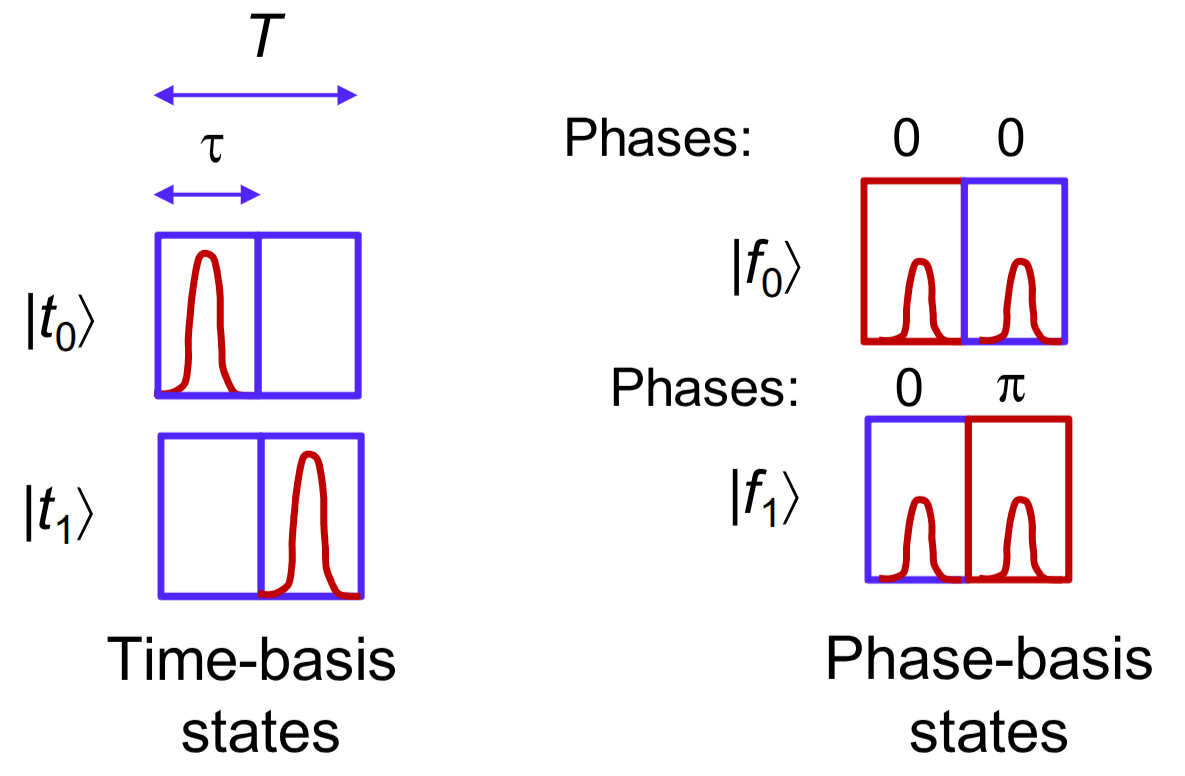
\includegraphics[width=0.8\textwidth]{chapters/figs/fig-6-7}
	\caption{حالت‌های کدگذاری فاز-زمان مورد استفاده در پروتکل \lr{BB84}.}
	\label{fig:6-7}
\end{figure}

\begin{figure}[ht]
	\centering
	 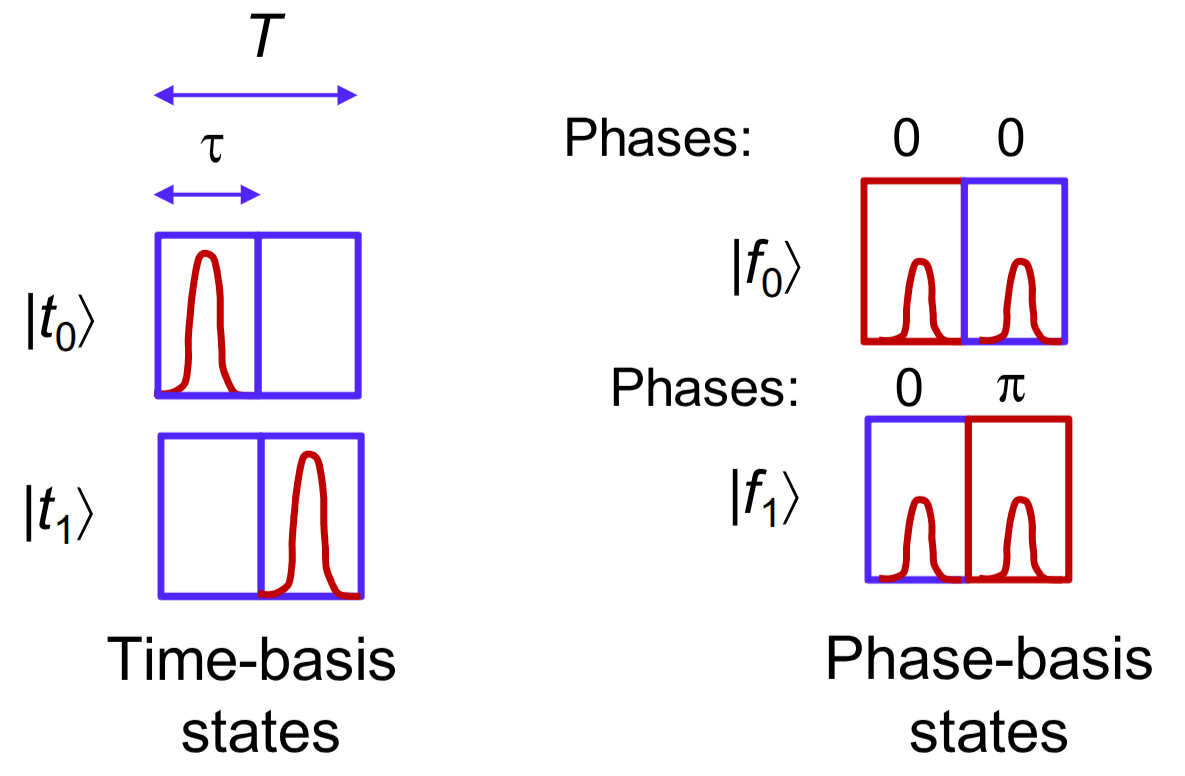
\includegraphics[width=0.8\textwidth]{chapters/figs/fig-6-8}
	\caption{رمزگذار فاز-زمان پروتکل توزیع کلید کوانتومی \lr{BB84}. \lr{AWG}: مولد شکل‌موج دلخواه؛ \lr{VOA}: تضعیف‌کننده نوری متغیر.}
	\label{fig:6-8}
\end{figure}

\begin{figure}[ht]
	\centering
	 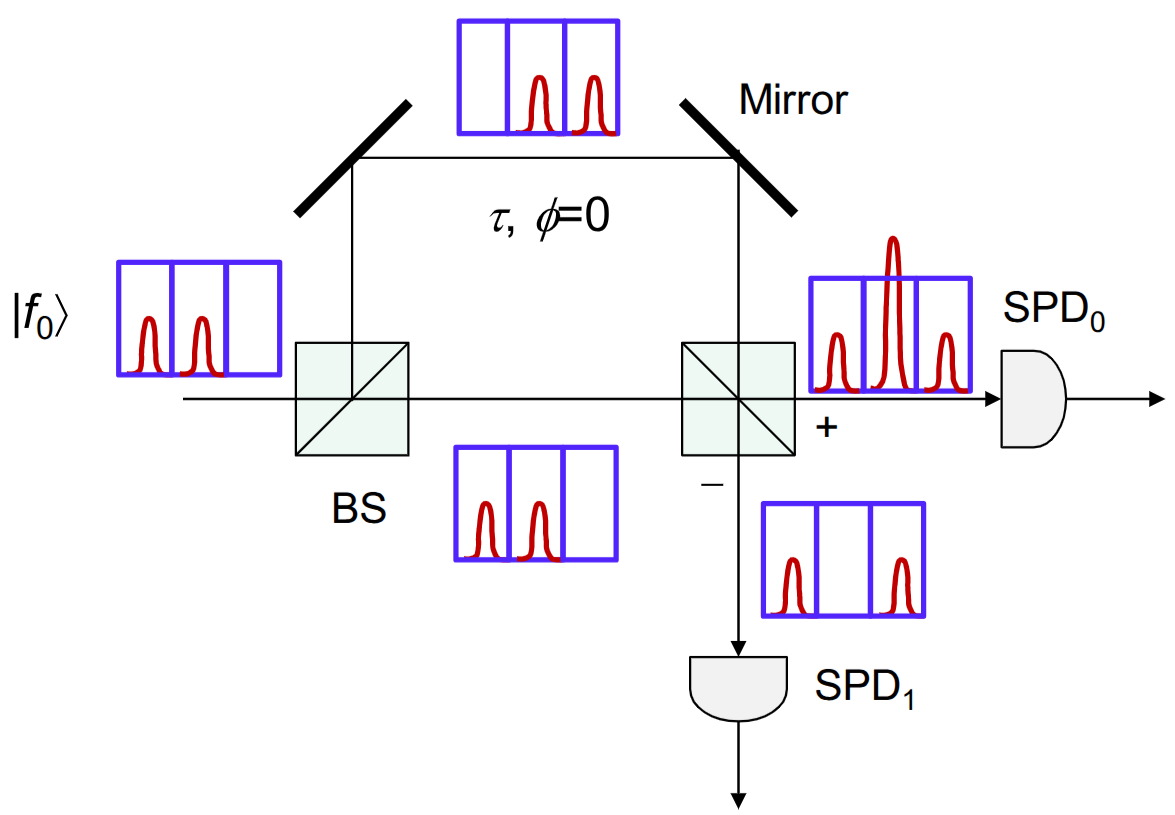
\includegraphics[width=0.8\textwidth]{chapters/figs/fig-6-9}
	\caption{رمزگشای فاز-زمان برای پروتکل توزیع کلید کوانتومی \lr{BB84}. \lr{BS}: تقسیم‌کننده پرتو $50:50$؛ \lr{SPD}: آشکارساز تک‌فوتون.}
	\label{fig:6-9}
\end{figure}

هنگامی که حالت فازی $|\phi_0\rangle$ به رمزگشای فاز-زمان وارد می‌شود، خروجی‌های دومین تقسیم‌کننده پرتو (\lr{BS}) ۵۰:۵۰ سه بازه زمانی را اشغال می‌کنند. خروجی $+$ موردی را نشان می‌دهد که در آن خروجی‌های تداخل‌سنج تداخل سازنده\LTRfootnote{Constructive interference} دارند، در حالی که خروجی $-$ نشان‌دهنده تداخل ویرانگر\LTRfootnote{Destructive interference} خروجی‌های متناظر تداخل‌سنج است. برای تداخل سازنده، پالس میانی دوبرابر می‌شود، در حالی که برای تداخل ویرانگر، پالس‌های میانی یکدیگر را خنثی می‌کنند. بنابراین، کلیک \lr{SPD} در بازه میانی در خروجی $+$، حالت $|\phi_0\rangle$ را شناسایی می‌کند و کلیک متناظر در خروجی $-$، حالت $|\phi_1\rangle$ را تشخیص می‌دهد.

\section{امنیت توزیع کلید کوانتومی}
\label{sec:6-5}
همان‌طور که در بخش مربوط به پروتکل \lr{BB84} بحث شد، آلیس و باب پس از اتمام مرحله ارسال کلید خام، فرآیند غربال‌گری و تخمین پارامتر\LTRfootnote{Parameter estimation} را انجام می‌دهند. از $N$ نماد ارسال شده، $n$ نماد باقی می‌ماند و کلید متناظر با آن‌ها، کلید غربال‌شده\LTRfootnote{Sifted key} نامیده می‌شود. پس از آن، آن‌ها پس‌پردازش کلاسیک مانند مصالحه اطلاعات و تقویت حریم خصوصی را انجام می‌دهند. در مرحله مصالحه اطلاعات، آن‌ها از تصحیح خطا برای اصلاح خطاهای ایجاد شده توسط کانال کوانتومی و ایو استفاده می‌کنند؛ کلید متناظر پس از اتمام این مرحله معمولاً کلید اصلاح‌شده\LTRfootnote{Corrected key} نامیده می‌شود. در طول تقویت حریم خصوصی، آن‌ها همبستگی باقی‌مانده با ایو را حذف می‌کنند و از $n$ نماد، $m$ نماد باقی می‌ماند که کلید متناظر، کلید امن\LTRfootnote{Secure key} است. به‌وضوح، نرخ کسر کلید مخفی $r$ را می‌توان به‌صورت $r = m/n$ (یا $m/N$) تعیین کرد که اغلب به آن کسر مخفی\LTRfootnote{Secret fraction} گفته می‌شود \cite{48}. نرخ کلید مخفی (\lr{SKR})\LTRfootnote{Secret-key rate (SKR)} سپس به‌صورت حاصل‌ضرب کسر مخفی $r$ و نرخ کلید خام $R_{\text{raw}}$ تعیین می‌شود و می‌توانیم بنویسیم \cite{48}:
\begin{equation}
	\text{SKR} = r \cdot R_{\text{raw}}
	\label{eq:6-22}
\end{equation}
جالب است که در بسیاری از مقالات، \lr{SKR} به همان کسر مخفی $r$ اشاره دارد. با توجه به اینکه نرخ کلید خام توسط دستگاه‌های مورد استفاده (به‌ویژه \lr{SPD}) و کانال کوانتومی که ارسال در آن صورت می‌گیرد تعیین می‌شود و نه توسط قوانین فیزیک کوانتوم، نرخ کسری را می‌توان نرخ \lr{SKR} نرمالیزه‌شده نیز نامید، به‌طوری که $r = \text{SKR}/R_{\text{raw}}$.

نرخ کلید خام را می‌توان به‌صورت حاصل‌ضرب نرخ سیگنال‌دهی $R_s$ و احتمال پذیرش نماد ارسالی توسط باب به‌طور میانگین، که با $\text{Pr}(\text{Bob accepting})$ نشان داده می‌شود، تعیین کرد؛ بنابراین می‌توانیم بنویسیم:
\begin{equation}
	R_{\text{raw}} = R_s \cdot \text{Pr}(\text{Bob accepting})
	\label{eq:6-23}
\end{equation}
از سوی دیگر، نرخ سیگنال‌دهی به‌صورت زیر تعیین می‌شود \cite{48}:
\begin{equation}
	R_s = \min \left\{ R_{s,\text{max}}, \frac{1}{T_{dc}}, \frac{1}{\mu T T_B \eta \tau_{\text{dead}}} \right\}
	\label{eq:6-24}
\end{equation}
که در آن $R_{s,\text{max}}$ حداکثر نرخ سیگنال‌دهی مجاز توسط منبع، $T_{dc}$ چرخه کاری\LTRfootnote{Duty cycle} و $\tau_{\text{dead}}$ زمان مرده\LTRfootnote{Dead time} مربوط به \lr{SPD} (زمان مورد نیاز برای بازنشانی \lr{SPD} پس از آشکارسازی یک فوتون) است. عبارت $\mu T T_B \eta$ متناظر با احتمال آشکارسازی باب است؛ $\mu$ میانگین تعداد فوتون‌های تولید شده توسط منبع، $\eta$ بازدهی \lr{SPD}، $T$ گذردهی\LTRfootnote{Transmissivity} کانال کوانتومی و $T_B$ نشان‌دهنده تلفات در گیرنده باب است. کانال کوانتومی معمولاً یک فیبر نوری یا یک کانال نوری فضای آزاد است. تضعیف در کانال فیبر نوری با $T = 10^{-\alpha L/10}$ تعیین می‌شود که در آن $\alpha$ ضریب تضعیف برحسب \lr{dB/km} و $L$ مسافت ارسال برحسب \lr{km} است. ضریب تضعیف معمول در فیبر تک‌مد استاندارد (\lr{SSMF})\LTRfootnote{Standard single-mode fiber (SSMF)} در طول موج ۱۵۵۰ نانومتر، $0.2$ \lr{dB/km} است. در مورد پیوند \lr{FSO}، اگر از اثرات تلاطم اتمسفری صرف‌نظر کنیم، برای یک پیوند خط دید\LTRfootnote{Line-of-sight} با مسافت ارسال $L$، می‌توانیم تلفات پیوند \lr{FSO} را طبق مرجع \cite{49} به‌صورت زیر تخمین بزنیم:
\begin{equation*}
	T = \left[ \frac{d_{Rx}}{d_{Tx} + DL} \right]^2 \cdot 10^{-\alpha L/10}
\end{equation*}
که در آن $d_{Tx}$ و $d_{Rx}$ قطر دهانه تلسکوپ‌های فرستنده و گیرنده و $D$ واگرایی\LTRfootnote{Divergence} است. بنابراین، جمله اول نشان‌دهنده تلفات هندسی و جمله دوم تضعیف میانگین ناشی از پراکندگی\LTRfootnote{Scattering} است، که ضریب تضعیف پراکندگی در شرایط آسمان صاف در محدوده ۱۵۲۰ تا ۱۶۰۰ نانومتر کمتر از $0.1$ \lr{dB/km} است.

در پروتکل \lr{BB84}، احتمالی که باب نماد ارسالی را می‌پذیرد به احتمال استفاده او از پایه یکسان مربوط است که با $p_{\text{sift}}$ نشان داده می‌شود، به‌طوری که نرخ سیگنال‌دهی به‌صورت $R_s p_{\text{sift}}$ در می‌آید و نرخ کلید خام زمانی که آلیس $n$ فوتون برای باب ارسال می‌کند، برابر خواهد بود با \cite{48}:


\begin{equation}
	R_{\text{raw},n} = R_s p_{\text{sift}} p_{A,n} p_n
	\label{eq:6-25}
\end{equation}
که در آن $p_{A,n}$ احتمال این است که پالس ارسال شده توسط آلیس شامل $n$ فوتون باشد (بخش زیر را ببینید) و $p_n$ احتمال این است که ایو پالسی با $n$ فوتون برای باب ارسال کند. نرخ کلید خام کل برابر با $R_{\text{raw}} = \sum_n R_{\text{raw},n}$ خواهد بود.

آنچه باقی مانده، تعیین نرخ کسر (تفاضلی) است. \lr{QKD} می‌تواند به امنیت غیرمشروط\LTRfootnote{Unconditional security} دست یابد، به این معنی که امنیت آن بدون اعمال هیچ‌گونه محدودیتی بر توان محاسباتی یا استراتژی شنود ایو، قابل تأیید است. کران‌های نرخ کسر به مراحل پس‌پردازش کلاسیک بستگی دارد. رایج‌ترین روش، پس‌پردازش یک‌طرفه\LTRfootnote{One-way postprocessing} است که در آن آلیس یا باب کلید مرجع را نگه داشته و اطلاعات کلاسیک را از طریق کانال عمومی برای طرف دیگر ارسال می‌کند، در حالی که طرف مقابل بدون ارائه بازخورد، فرآیند خاصی را روی داده‌ها انجام می‌دهد. معمول‌ترین پردازش یک‌طرفه شامل دو مرحله مصالحه اطلاعات و تقویت حریم خصوصی است. رابطه کسر مخفی به‌دست‌آمده از پس‌پردازش یک‌طرفه در مرجع \cite{48} به‌صورت زیر داده شده است:
\begin{equation}
	r = I(\bm{A}; \bm{B}) - \min_{\text{Eve's strategies}} (I_{EA}, I_{EB})
	\label{eq:6-26}
\end{equation}
که در آن $I(\bm{A}; \bm{B})$ اطلاعات متقابل بین آلیس و باب است، در حالی که جمله دوم متناظر با اطلاعات ایو $I_E$ درباره کلید خام آلیس یا باب است و کمینه‌سازی روی تمام استراتژی‌های شنود ممکن انجام می‌شود. آلیس و باب تصمیم می‌گیرند که از مصالحه مستقیم یا معکوس استفاده کنند تا بتوانند اطلاعات ایو را کمینه کنند.

اکنون استراتژی‌های مختلف شنود را که ایو ممکن است به کار گیرد و اطلاعات ایو $I_E$ را تعیین می‌کنند، شرح می‌دهیم.

\subsubsection{حملات مستقل (انفرادی) یا غیرهمدوس}
\label{subsec:6-5-1}
این محدودترین خانواده از حملات است که در آن ایو به هر کیوبیت به‌طور مستقل حمله کرده و با اعمال استراتژی یکسان با هر کیوبیت تعامل می‌کند. علاوه بر این، او حالت‌های کوانتومی را پیش از انجام پس‌پردازش کلاسیک اندازه‌گیری می‌کند. کران امنیت برای حملات غیرهمدوس\LTRfootnote{Incoherent attacks} مشابه امنیت لایه فیزیکی (\lr{PLS}) کلاسیک \cite{2} است و توسط حد سیزار-کورنر\LTRfootnote{Csiszár-Körner bound} \cite{50} تعیین می‌شود که در رابطه \eqref{eq:6-26} داده شده است و در آن اطلاعات متقابل بین آلیس و ایو به‌صورت زیر است:
\begin{equation}
	I_{EA} = \max_{\text{Eve's strategies}} I(\bm{A}; \bm{E})
	\label{eq:6-27}
\end{equation}
که در آن بیشینه‌سازی روی تمام استراتژی‌های شنود غیرهمدوس ممکن انجام می‌شود. تعریف مشابهی برای $I_{BE}$ نیز برقرار است.

خانواده مهمی از حملات غیرهمدوس، حملات سد کردن-بازارسال\LTRfootnote{Intercept-resend (IR) attacks} (\lr{IR}) هستند؛ که در آن ایو سیگنال کوانتومی ارسال شده توسط آلیس را سد کرده، اندازه‌گیری را روی آن انجام می‌دهد و بر اساس نتیجه اندازه‌گیری، سیگنال کوانتومی جدیدی را (در همان \lr{MUB} حالت کوانتومی اندازه‌گیری شده) آماده کرده و آن را برای باب ارسال می‌کند. در پروتکل \lr{BB84}، انتخاب پایه توسط ایو در ۵۰٪ مواقع با پایه آلیس مطابقت دارد. زمانی که او از پایه اشتباه استفاده می‌کند، باز هم ۵۰٪ شانس برای حدس زدن بیت صحیح دارد. وقتی باب اندازه‌گیری را انجام می‌دهد، ۵۰٪ احتمال دارد که باب از همان پایه ایو استفاده کند. با این حال، این بیت‌ها با دنباله ایو همبستگی خواهند داشت و نه با آلیس، و احتمال کلی خطا ۱/۴ خواهد بود، در حالی که اطلاعات متقابل بین آلیس و ایو $I(\bm{A}; \bm{E}) = 1/2$ است. با توجه به احتمال خطای بالای ایجاد شده توسط حمله \lr{IR}، آلیس و باب می‌توانند به راحتی فعالیت ایو را شناسایی کنند. با این حال، ایو ممکن است تصمیم بگیرد حمله \lr{IR} را با احتمال $p_{IR}$ اعمال کند. در آن صورت احتمال خطا $q = p_{IR}/4$ خواهد بود. اطلاعات متقابل بین آلیس و ایو در این صورت $I(\bm{A}; \bm{E}) = h(p_{IR}/4)$ خواهد بود، که در آن $h(\cdot)$ تابع آنتروپی باینری\LTRfootnote{Binary entropy function} $h(q) = -q \log_2 q - (1-q) \log_2 (1-q)$ است. اگر تمام خطاها به ایو نسبت داده شود، کسر مخفی را می‌توان به‌صورت زیر تخمین زد:
\begin{equation}
	r = \underbrace{1 - h(q)}_{I(\bm{A}; \bm{B})} - h(q) = 1 - 2h(q)
	\label{eq:6-28}
\end{equation}

خانواده مهم دیگری از حملات غیرهمدوس، حملات \lr{PNS} هستند \cite{51} که در آن ایو روی حالت‌های کوانتومی چندفوتونی عمل می‌کند. در یک سیستم \lr{QKD} مبتنی بر \lr{WCS}، حالت‌های کوانتومی با مدوله کردن باریکه از منبع نور همدوس تولید می‌شوند که سپس تضعیف می‌گردد تا به‌طور میانگین یک فوتون در هر پالس توسط آلیس ارسال شود. با این حال، همان‌طور که پیش‌تر بحث شد، منبع همدوس فوتون‌ها را بر اساس توزیع پواسون گسیل می‌کند، به‌طوری که احتمال گسیل $n$ فوتون در حالتی با میانگین تعداد فوتون تولید شده $\mu$ توسط معادله زیر تعیین می‌شود:
\begin{equation}
	p_{A,n} = p(n|\mu) = \frac{e^{-\mu} \mu^n}{n!}
	\label{eq:6-29}
\end{equation}
با افزایش پارامتر $\mu$، احتمال دریافت بیش از یک فوتون نیز افزایش می‌یابد. برای انجام حمله \lr{PNS}، ایو می‌تواند از تقسیم‌کننده پرتو برای برداشتن یکی از فوتون‌ها از حالت چندفوتونی استفاده کند و بقیه را به باب انتقال دهد، همان‌طور که در شکل \ref{fig:6-10} تصویر شده است. او می‌تواند فوتون را با انتخاب تصادفی پایه اندازه‌گیری کند. ایو حتی می‌تواند پیوند کوانتومی را با فیبر با تلفات بسیار کم جایگزین کند تا آلیس و باب نتوانند تشخیص دهند که سیگنال ارسالی تضعیف شده است. برای حل مشکل حمله \lr{PNS}، آلیس و باب می‌توانند از پروتکل مبتنی بر حالت فریب \cite{37} استفاده کنند که در آن آلیس حالت‌های کوانتومی را با میانگین تعداد فوتون‌های متفاوت (نشان‌دهنده حالت‌های سیگنال و فریب) ارسال می‌کند. ایو نمی‌تواند بین حالت‌های فریب و سیگنال تمایز قائل شود و با توجه به اینکه آلیس و باب سطح سیگنال فریب را می‌دانند، می‌توانند حمله \lr{PNS} را شناسایی کنند.

\subsubsection{حملات دسته‌جمعی}
\label{subsec:6-5-2}
حملات دسته‌جمعی\LTRfootnote{Collective attacks} نشان‌دهنده تعمیمی از حملات غیرهمدوس هستند، با این فرض که تعامل ایو با هر کیوبیت نیز به‌صورت مستقل و با توزیع یکسان (\lr{i.i.d.})\LTRfootnote{Independent and identically distributed (i.i.d.)} است. با این حال، در این حملات، ایو می‌تواند کیوبیت‌های کمکی\LTRfootnote{Ancilla qubits} خود را تا پایان مراحل پس‌پردازش کلاسیک در یک حافظه کوانتومی ذخیره کند. برای مثال، با توجه به اینکه مصالحه اطلاعات مستلزم تبادل بیت‌های توازن\LTRfootnote{Parity bits} روی یک کانال کلاسیک احرازهویت‌شده است، ایو می‌تواند بهترین حملات کلاسیک شناخته‌شده را برای یادگیری محتوای بیت‌های توازن به کار گیرد. بر اساس تمام اطلاعات در دسترس، ایو می‌تواند بهترین استراتژی اندازه‌گیری را روی کیوبیت‌های کمکی خود (ذخیره شده در حافظه کوانتومی) انجام دهد.

حمله \lr{PNS} زمانی که ایو از حافظه کوانتومی استفاده می‌کند قوی‌تر است. به‌ویژه، ایو می‌تواند از طریق فرآیند غربال‌گری متوجه شود که کدام پایه توسط آلیس استفاده شده است و می‌تواند پایه صحیح را روی فوتون ذخیره شده در حافظه کوانتومی خود اعمال کند و در نتیجه تعداد بیت‌های شناسایی شده را در مقایسه با حالتی که از حافظه کوانتومی استفاده نمی‌شود، دوبرابر کند.

کران امنیت برای حملات دسته‌جمعی، با فرض پس‌پردازش یک‌طرفه، توسط رابطه \eqref{eq:6-26} داده می‌شود که در آن اطلاعات ایو درباره دنباله آلیس از طریق اطلاعات هولِوو\LTRfootnote{Holevo information} به‌صورت زیر تعیین می‌شود \cite{52}:

\begin{figure}[ht]
	\centering
	 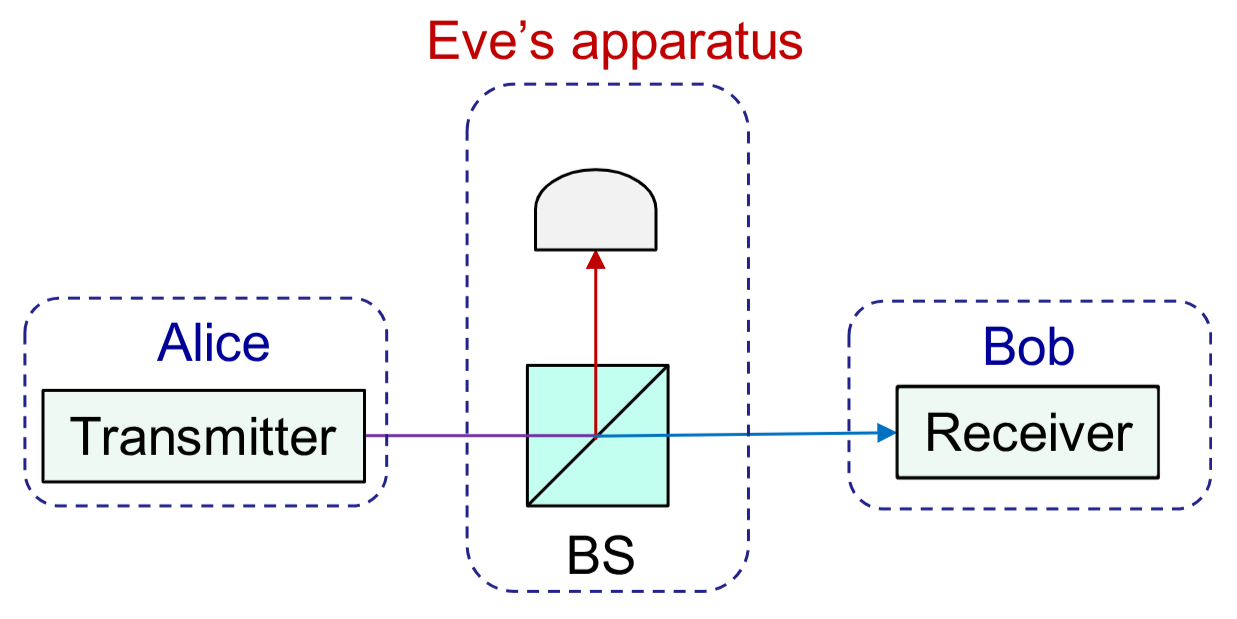
\includegraphics[width=0.7\textwidth]{chapters/figs/fig-6-10}
	\caption{تصویرسازی اجرای حمله تقسیم تعداد فوتون توسط ایو. \lr{BS}: تقسیم‌کننده پرتو.}
	\label{fig:6-10}
\end{figure}



\begin{equation}
	I_{EA} = \max_{\text{Eve's strategies}} \chi(\bm{A}; \bm{E})
	\label{eq:6-30}
\end{equation}
که در آن بیشینه‌سازی روی تمام استراتژی‌های شنود دسته‌جمعی ممکن انجام می‌شود. این کران با نام کران دوتک-وینتر\LTRfootnote{Devetak-Winter bound} نیز شناخته می‌شود. اطلاعات هولِوو که در مرجع \cite{53} معرفی شده است، در اینجا به‌صورت زیر تعریف می‌شود:
\begin{equation}
	\chi(\bm{A}; \bm{E}) = S(\rho_E) - \sum_a p(a) S(\rho_{E|a})
	\label{eq:6-31}
\end{equation}
که در آن $S(\rho)$ آنتروپی فون نویمان\LTRfootnote{von Neumann entropy} است که به‌صورت $S(\rho) = -\text{Tr}(\rho \log \rho) = -\sum_i \lambda_i \log \lambda_i$ تعریف می‌شود و در آن $\lambda_i$ مقادیر ویژه عملگر (حالت) چگالی $\rho$ هستند. در رابطه \eqref{eq:6-31}، $p(a)$ نشان‌دهنده احتمال وقوع نماد $a$ از الفبای کلاسیک آلیس است، در حالی که $\rho_{E|a}$ عملگر چگالی متناظر با سیستم کمکی\LTRfootnote{Ancilla} ایو است. در نهایت، $\rho_E$ حالت چگالی جزئی ایو است که به‌صورت $\rho_E = \sum_a p(a) \rho_{E|a}$ تعریف می‌شود. به عبارت دیگر، اطلاعات هولِوو متناظر با میانگین کاهش در آنتروپی فون نویمان است، با این فرض که می‌دانیم $\rho_E$ چگونه آماده‌سازی شده است.



\subsubsection{حملات هک کوانتومی و حملات کانال جانبی}
\label{subsec:6-5-3}
حملات هک کوانتومی\LTRfootnote{Quantum hacking attacks} از نقاط ضعف پیاده‌سازی‌های خاص سیستم‌های \lr{QKD} بهره‌برداری می‌کنند. بسیاری از این حملات هک با فناوری کنونی امکان‌پذیر هستند. در یک حمله اسب تروا\LTRfootnote{Trojan horse attack} \cite{54}، ایو یک باریکه لیزری درخشان را به سمت رمزگذار آلیس می‌فرستد و فوتون‌های بازتابیده را برای کسب اطلاعات درباره کلید مخفی اندازه‌گیری می‌کند. با استفاده از یک ایزولاتور نوری\LTRfootnote{Optical isolator} می‌توان از این حمله جلوگیری کرد. همچنین مشاهده شده است که شمارنده‌های فوتون مبتنی بر سیلیسیم که از فوتودیودهای بهمنی\LTRfootnote{Avalanche photodiodes (APDs)} (\lr{APD}) استفاده می‌کنند، هنگام آشکارسازی یک تک‌فوتون، مقداری نور در طول‌موج‌های مختلف ساطع می‌کنند که می‌تواند توسط ایو مورد بهره‌برداری قرار گیرد \cite{55}. در حمله جابه‌جایی زمانی\LTRfootnote{Time-shifting attack} \cite{56}، ایو از عدم تطابق بازدهی \lr{SPD}های باب برای تخمین انتخاب پایه توسط او استفاده می‌کند. در یک حمله کورسازی\LTRfootnote{Blinding attack} \cite{57}، ایو از ویژگی‌های شمارنده تک‌فوتون مبتنی بر \lr{APD} بهره می‌گیرد تا باب را مجبور کند همان پایه‌ای را انتخاب کند که ایو انتخاب کرده است. \lr{APD}ها برای شمارش فوتون اغلب در مد گیت‌شده\LTRfootnote{Gated mode} عمل می‌کنند، به این معنی که \lr{APD} تنها زمانی فعال است که انتظار ورود فوتون می‌رود. وقتی \lr{APD} در وضعیت غیرفعال (خاموش) است، در یک رژیم خطی\LTRfootnote{Linear regime} عمل می‌کند، به این معنی که جریان نوری با توان نوری دریافتی متناسب است و بنابراین مانند یک فتودتکتور کلاسیک رفتار می‌کند. برای بهره‌برداری از این موضوع، ایو می‌تواند یک باریکه نور کلاسیک ضعیف ارسال کند که به اندازه کافی قوی باشد تا زمانی که باب از همان پایه ایو استفاده می‌کند «کلیک» ایجاد کند، و در غیر این صورت کلیکی ثبت نشود. در چنین سناریویی، ۵۰٪ از رویدادها به عنوان بی‌نتیجه ثبت می‌شوند. خوشبختانه، ویژگی مشترک حملات هک کوانتومی این است که به محض شناخته شدن حمله، قابل پیشگیری هستند. با این حال، تهدید ناشی از حملات هک کوانتومی ناشناخته همچنان پابرجاست.

بسیاری از حملات کانال جانبی\LTRfootnote{Side-channel attacks} به‌طور هم‌زمان حملات زمان خطای صفر\LTRfootnote{Time zero-error attacks} هستند \cite{48}. به بیان دیگر، ایو می‌تواند از تلفات کانال کوانتومی برای پنهان کردن حمله کانال جانبی خود استفاده کند. حمله تقسیم پرتو\LTRfootnote{Beam-splitting attack} از تلفات کانال کوانتومی بهره‌برداری می‌کند؛ ایو می‌تواند یک تقسیم‌کننده پرتو را دقیقاً بعد از فرستنده آلیس قرار دهد، بخشی از باریکه را برداشته و بقیه را به باب انتقال دهد. از آنجا که آلیس مد نوری را تغییر نمی‌دهد، این حمله توسط باب شناسایی نخواهد شد. جالب اینجاست که توزیع پواسون در طول حمله \lr{PNS} حفظ می‌شود \cite{58}. در پیاده‌سازی‌های واقع‌گرایانه، زمانی که آلیس از حالت‌های سیگنال مستقل خطی استفاده می‌کند، ایو می‌تواند تمایز ابهام‌ناپذیر حالت\LTRfootnote{Unambiguous state discrimination} را انجام داده و متعاقب آن سیگنال را مجدداً ارسال کند و به بازدهی بهتری نسبت به تقسیم پرتو دست یابد، همان‌طور که در مرجع \cite{59} نشان داده شده است. خوشبختانه، وجود حملات کانال جانبی تا زمانی که حملات مربوطه در مرحله تقویت حریم خصوصی در نظر گرفته شوند، امنیت را به خطر نمی‌اندازد \cite{48}.

\subsubsection{امنیت پروتکل BB84}
\label{subsec:6-5-4}
کران پایین کسر مخفی که با پروتکل \lr{BB84} قابل دستیابی است، توسط رابطه زیر داده می‌شود:
\begin{equation}
	r = q(Z)_1 [1 - h_2(e(X)_1)] - f_e q(Z) h_2(e(Z))
	\label{eq:6-32}
\end{equation}
که در آن $q(Z)_1$ نشان‌دهنده احتمال اعلام یک نتیجه موفقیت‌آمیز («بهره»\LTRfootnote{Gain}) در زمانی است که آلیس یک تک‌فوتون ارسال کرده و باب آن را در پایه $Z$ آشکار کرده است؛ $f_e$ نشان‌دهنده ناکارآمدی تصحیح خطا ($f_e \geq 1$) است؛ $e(X)$ [$e(Z)$] نشان‌دهنده نرخ خطای بیت کوانتومی\LTRfootnote{Quantum bit error rate (QBER)} (\lr{QBER}) در پایه $X$ (پایه $Z$) است؛ و $h_2(x)$ تابع آنتروپی باینری است که به‌صورت زیر تعریف می‌شود:
\begin{equation}
	h_2(x) = -x \log_2(x) - (1-x) \log_2(1-x)
	\label{eq:6-33}
\end{equation}
جمله دوم یعنی $q(Z)_1 h_2[e(X)_1]$ نشان‌دهنده مقدار اطلاعاتی است که ایو توانسته در طول ارسال کلید خام به‌دست آورد و این اطلاعات معمولاً در مرحله تقویت حریم خصوصی از کلید نهایی حذف می‌شود. جمله آخر یعنی $f_e q(Z) h_2[e(Z)]$ نشان‌دهنده مقدار اطلاعات فاش شده در مرحله مصالحه اطلاعات (تصحیح خطا) است که معمولاً به بیت‌های توازن تبادل شده در یک کانال عمومی بدون نویز مربوط می‌شود (زمانی که از تصحیح خطای سیستماتیک استفاده می‌شود).

\section{پروتکل‌های حالت فریب}
\label{sec:6-6}
هنگامی که به جای یک منبع تک‌فوتون از یک منبع حالت همدوس ضعیف (\lr{WCS}) استفاده می‌شود، این طرح نسبت به حمله \lr{PNS} حساس خواهد بود. با توجه به اینکه احتمال ارسال چندین فوتون از \lr{WCS} اکنون غیرصفر است، ایو می‌تواند از این واقعیت برای کسب اطلاعات از کانال بهره‌برداری کند. برای غلبه بر حمله \lr{PNS}، استفاده از سیستم‌های توزیع کلید کوانتومی مبتنی بر حالت فریب\LTRfootnote{Decoy-state} در مراجع \cite{37, 61, 62, 63, 64, 65, 66, 67, 68, 69, 70} پیشنهاد شده است. در \lr{QKD} حالت فریب، میانگین تعداد فوتون‌های ارسالی در بازه‌های زمانی تصادفی افزایش می‌یابد که به آلیس و باب اجازه می‌دهد تشخیص دهند که آیا در زمان ارسال چندین فوتون، ایو در حال سرقت فوتون‌ها است یا خیر. نسخه‌های مختلفی از پروتکل‌های مبتنی بر حالت فریب وجود دارد. در پروتکل مبتنی بر یک-حالت-فریب، علاوه بر حالت سیگنال با میانگین تعداد فوتون $\mu$، حالت فریب با میانگین تعداد فوتون $\nu < \mu$ نیز به کار گرفته می‌شود. آلیس ابتدا درباره سطوح میانگین تعداد فوتون سیگنال و فریب تصمیم‌گیری کرده و سپس بر اساس رابطه \lr{SKR} متناظر، احتمالات بهینه برای استفاده از این دو سطح را تعیین می‌کند. در پروتکل مبتنی بر «حالت فریب ضعیف به‌علاوه خلاء»، علاوه بر سطوح $\mu$ و $\nu$، از حالت خلاء\LTRfootnote{Vacuum state} نیز به عنوان حالت فریب استفاده می‌شود. هر دو پروتکل در مرجع \cite{67} به‌صورت تئوری و تجربی ارزیابی شده‌اند. نتیجه‌گیری شد که استفاده از یک حالت سیگنال و دو حالت فریب کافی است، که این موضوع با یافته‌های مراجع \cite{68, 69} مطابقت دارد.

احتمالی که آلیس بتواند فوتون را با موفقیت آشکارسازی کند، زمانی که از \lr{WCS} با میانگین تعداد فوتون $\mu$ استفاده می‌کند، با $q_\mu$ نشان داده می‌شود و به عنوان بهره\LTRfootnote{Gain} شناخته می‌شود که می‌تواند توسط رابطه زیر تعیین گردد:
\begin{equation}
	q_\mu = \sum_{n=0}^{\infty} y_n \frac{e^{-\mu} \mu^n}{n!}
	\label{eq:6-34}
\end{equation}
که در آن $y_n$، که به عنوان بازده\LTRfootnote{Yield} نیز شناخته می‌شود، احتمال آشکارسازی موفقیت‌آمیز باب در زمانی است که آلیس $n$ فوتون ارسال کرده است. رابطه مشابهی برای حالت‌های فریب با میانگین تعداد فوتون $\nu_i$ برقرار است، یعنی:
\begin{equation}
	q_{\nu_i} = \sum_{n=0}^{\infty} y_n \frac{e^{-\nu_i} \nu_i^n}{n!}
	\label{eq:6-35}
\end{equation}

اگر $e_n$ نشان‌دهنده \lr{QBER} متناظر با حالتی باشد که آلیس $n$ فوتون ارسال کرده است، میانگین \lr{QBER} برای حالت همدوس $|\sqrt{\mu} \exp(j\phi)\rangle$ (که در آن $\phi$ فاز دلخواه است) را می‌توان به‌صورت زیر تخمین زد:
\begin{equation}
	e_\mu = \frac{1}{q_\mu} \sum_{n=0}^{\infty} y_n e_n \frac{e^{-\mu} \mu^n}{n!}
	\label{eq:6-36}
\end{equation}

اگر $\eta_{\text{all}}$ بازدهی کل ارسال، متشکل از گذردهی کانال $T_{ch}$، بازدهی فتودتکتور $\eta$ و گذردهی بخش نوری باب $T_{\text{Bob}}$ باشد، بازدهی ارسال پالس $n$-فوتونی به‌صورت زیر خواهد بود:
\begin{equation}
	T_n = 1 - (1 - \eta_{\text{all}})^n
	\label{eq:6-37}
\end{equation}

در غیاب ایو، برای $n=0$، بازده $y_0$ تحت تأثیر نرخ آشکارسازی پس‌زمینه که با $p_d$ نشان داده می‌شود، قرار دارد؛ بنابراین می‌توانیم بنویسیم $y_0 = p_d$. از سوی دیگر، بازده برای $n \geq 1$ توسط هر دو عامل فوتون‌های سیگنال و نرخ پس‌زمینه به صورت زیر تعیین می‌شود:
\begin{equation}
	y_n = T_n + y_0 - T_n y_0 = T_n + y_0(1 - T_n) = 1 - (1 - y_0)(1 - \eta_{\text{all}})^n
	\label{eq:6-38}
\end{equation}

نرخ خطای حالت‌های $n$-فوتونی $e_n$ را می‌توان طبق مراجع \cite{37, 70} به‌صورت زیر تخمین زد:
\begin{equation}
	e_n = \frac{1}{y_n} \left[ e_0 y_0 + e_d T_n \right] \approx e_d + \frac{y_0}{y_n} (e_0 - e_d)
	\label{eq:6-39}
\end{equation}
که در آن $e_d$ احتمال برخورد یک فوتون به یک آشکارساز اشتباه است. برای کدگذاری فاز-زمان، این مقدار نشان‌دهنده نرخ خطای عدم انطباق ذاتی\LTRfootnote{Intrinsic misalignment error rate} است. در غیاب فوتون‌های سیگنال، با فرض اینکه دو آشکارساز دارای نرخ‌های پس‌زمینه یکسانی هستند، می‌توانیم بنویسیم $e_0 = 1/2$. به‌طور مشابه، میانگین \lr{QBER} را می‌توان به‌صورت زیر تخمین زد:
\begin{equation}
	e_\mu = e_d + \frac{y_0}{q_\mu} (e_0 - e_d)
	\label{eq:6-40}
\end{equation}

اکنون می‌توان کران پایین کسر امنیت را با اصلاح رابطه مربوط به پروتکل‌های \lr{BB84} به‌صورت زیر تعیین کرد:
\begin{equation}
	r = q(Z)_1 [1 - h_2(e(X)_1)] - q(Z)_\mu f_e h_2(e(Z)_\mu)
	\label{eq:6-41}
\end{equation}
که در آن زیرنویس $1$ نشان‌دهنده پالس‌های تک‌فوتونی و زیرنویس $\mu$ نشان‌دهنده پالسی با میانگین تعداد فوتون $\mu$ است.

به‌عنوان یک نمونه، شکل \ref{fig:6-11} نتایج کسر امنیت را برای پروتکل حالت فریب و پروتکل آماده‌سازی-و-اندازه‌گیری \lr{BB84} مبتنی بر \lr{WCS}، با فرض استفاده از فیبر تک‌مد استاندارد (\lr{SMF}) با ضریب تضعیف $0.21$ \lr{dB/km} ارائه می‌دهد.

سایر پارامترهای استفاده شده در شبیه‌سازی‌ها به‌صورت زیر تنظیم شده‌اند \cite{37, 71, 72, 73}: بازدهی آشکارساز $\eta = 0.045$، نرخ شمارش تاریک $p_d = 1.7 \times 10^{-6}$، احتمال برخورد فوتون به آشکارساز اشتباه $e_d = 0.033$ و ناکارآمدی مصالحه $f_e = 1.22$. برای پروتکل \lr{BB84} مبتنی بر حالت فریب، جهت محاسبه کسر امنیت، از رابطه \eqref{eq:6-41} برای مقدار بهینه میانگین تعداد فوتون در هر پالس $\mu$ استفاده می‌کنیم که در آن $q_\mu$ توسط $q_\mu = 1 - (1 - y_0)\exp(-\mu \eta_{\text{all}})$ تعیین می‌شود، $e_\mu$ توسط رابطه \eqref{eq:6-40}، $e_1$ توسط رابطه \eqref{eq:6-39} و $q_1$ به عنوان آرگومان \eqref{eq:6-34} برای $n=1$ یعنی توسط $q_1 = y_1 \mu \exp(-\mu)$ تعیین می‌گردد. برای پروتکل \lr{BB84} مبتنی بر \lr{WCS} بدون حالت فریب، از رابطه \eqref{eq:6-41} با این فرض استفاده می‌کنیم که ایو کانال را کنترل می‌کند، حملات سد کردن-بازارسال را انجام می‌دهد و نسبت به حالت‌های چندفوتونی شفاف است. در این سناریوی کران پایین، خطای ناشی از رویدادهای تک‌فوتونی غالب است. اکنون با محاسبه $q(Z)$ توسط $q_\mu = 1 - (1 - y_0)\exp(-\mu \eta_{\text{all}})$ و $e(Z)$ توسط $E_\mu = e_d + (e_0 - e_d)y_0/q_\mu$ و با فرض $\mu$ غیربهینه متناسب با $\eta_{\text{all}}$، منحنی زرد رنگ در شکل \ref{fig:6-11} به‌دست آمد که با مرجع \cite{37} مطابقت دارد. هنگامی که به جای آن از $\mu$ بهینه (که کسر امنیت را بیشینه می‌کند) استفاده می‌کنیم، منحنی بنفش به‌دست می‌آید که با مرجع \cite{71} مطابقت دارد. برای این دو منحنی، مقدار $q(Z)_1$ را از \eqref{eq:6-34} با قرار دادن $y_n = 1$ برای $n \geq 2$ (ببینید مرجع \cite{70}) به‌صورت زیر تخمین می‌زنیم:
\begin{equation}
	q(X)_1 \approx q_\mu - \sum_{n=2}^{\infty} \frac{e^{-\mu} \mu^n}{n!}
	\label{eq:6-42}
\end{equation}
با توجه به اینکه حالت‌های چندفوتونی خطایی ایجاد نمی‌کنند (یعنی $e_n = 0$ برای $n \geq 2$)، می‌توانیم $e_1$ را به‌صورت زیر محدود کنیم:
\begin{equation}
	e(X)_1 \approx q_\mu E_\mu / q(X)_1
	\label{eq:6-43}
\end{equation}
رابطه دقیق‌تر برای $q_\mu$ در پروتکل \lr{BB84} مبتنی بر \lr{WCS} به‌صورت زیر خواهد بود:
\begin{equation}
	q_\mu = y_0 e^{-\mu} + y_1 e^{-\mu} \mu + \sum_{n=2}^{\infty} \frac{e^{-\mu} \mu^n}{n!}
	\label{eq:6-44}
\end{equation}
که از رابطه \eqref{eq:6-34} با قرار دادن $y_n = 1$ برای $n \geq 2$ به‌دست می‌آید. منحنی متناظر با رنگ صورتی نشان داده شده است که نشان می‌دهد با استفاده از پروتکل \lr{BB84} مبتنی بر \lr{WCS}، مسافت $L = 48.62$ کیلومتر قابل دستیابی است. در مقابل، برای پروتکل \lr{BB84} مبتنی بر حالت فریب و $\mu$ بهینه، دستیابی به مسافت نزدیک به $141.8$ کیلومتر امکان‌پذیر است (منحنی آبی را ببینید) که با مرجع \cite{71} مطابقت دارد.

\begin{figure}[ht]
	\centering
	 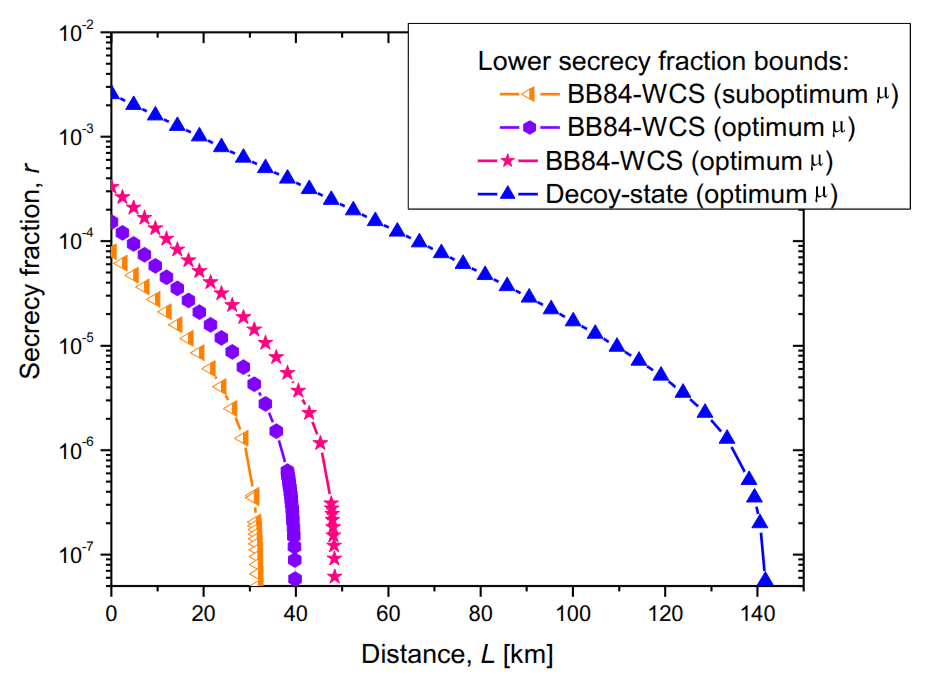
\includegraphics[width=0.8\textwidth]{chapters/figs/fig-6-11}
	\caption{کسر امنیت در مقابل مسافت ارسال برای پروتکل مبتنی بر حالت فریب و پروتکل \lr{BB84} مبتنی بر حالت همدوس ضعیف.}
	\label{fig:6-11}
\end{figure}


\section{پروتکل‌های توزیع کلید کوانتومی مستقل از دستگاه اندازه‌گیری}
\label{sec:6-7}
هرگونه اختلاف در پارامترهای دستگاه‌ها نسبت به فرضیات در نظر گرفته شده در پروتکل‌های \lr{QKD}، می‌تواند توسط مهاجمان از طریق حملات کانال جانبی و هک کوانتومی \cite{54,55,56,57,58} برای به مخاطره انداختن امنیت پروتکل‌های مربوطه مورد بهره‌برداری قرار گیرد. یکی از راه‌های حل این مشکل، ابداع روش‌های مختلف برای غلبه بر حملات شناخته‌شده‌ی کانال جانبی یا هک کوانتومی است. متأسفانه، شنودگر همیشه می‌تواند حملات پیچیده‌تری را طراحی کند. استراتژی دیگر و موثرتر، ابداع پروتکل‌های جدیدی است که در آن‌ها کمترین فرضیات درباره دستگاه‌های مورد استفاده در پروتکل در نظر گرفته شده باشد. یکی از این پروتکل‌ها با عنوان \lr{QKD} مستقل از دستگاه\LTRfootnote{Device-independent QKD (DI-QKD)} (\lr{DI-QKD}) شناخته می‌شود \cite{74,75,76,77} که در آن آمار آشکارسازی برای ایمن‌سازی کلید، بدون در نظر گرفتن هیچ فرضی در مورد عملکرد دستگاه‌ها تعیین شده است. در پروتکل‌های \lr{MDI-QKD}\LTRfootnote{Measurement-device-independent QKD (MDI-QKD)}، چارلی اندازه‌گیری‌های حالت بل (\lr{BSM}) را انجام داده و نتایج را اعلام می‌کند؛ به همین دلیل ابتدا به شرح \lr{BSM}ها می‌پردازیم.

\subsection{اندازه‌گیری‌های حالت بل فوتونی}
\label{subsec:6-7-1}
اندازه‌گیری‌های حالت بل\LTRfootnote{Bell state measurements (BSMs)} (\lr{BSM}) نقش کلیدی در محاسبات و ارتباطات کوانتومی فوتونی، از جمله دورنوردی کوانتومی \cite{78}، کدگذاری فوق‌فشرده\LTRfootnote{Superdense coding} \cite{79}، جابه‌جایی کوانتومی\LTRfootnote{Quantum swapping} \cite{80}، تکرارکننده‌های کوانتومی\LTRfootnote{Quantum repeaters} \cite{81} و \lr{QKD} \cite{82,83,84} ایفا می‌کنند. یک \lr{BSM} کامل نشان‌دهنده تصویر کردن هر حالتِ دوفوتونی بر حالت‌های بل بیشینه درهم‌تنیده\LTRfootnote{Maximally entangled Bell states} است که به‌صورت زیر تعریف می‌شوند:
\begin{equation}
	|\psi^{\pm}\rangle = \frac{1}{\sqrt{2}} (|01\rangle \pm |10\rangle); \quad |\phi^{\pm}\rangle = \frac{1}{\sqrt{2}} (|00\rangle \pm |11\rangle)
	\label{eq:6-45}
\end{equation}
متأسفانه، دستیابی به \lr{BSM} کامل تنها با استفاده از اپتیک خطی\LTRfootnote{Linear optics} و بدون فوتون‌های کمکی\LTRfootnote{Auxiliary photons} غیرممکن است. در مرجع \cite{85} نشان داده شده است که احتمال \lr{BSM} موفقیت‌آمیز برای دو فوتون که در حالت‌های ورودی کاملاً مخلوط\LTRfootnote{Complete mixed input states} هستند، به ۵۰٪ محدود می‌شود. رویکرد متداول برای تحلیل حالت بل، استفاده از یک \lr{BS} ۵۰:۵۰ و متعاقب آن استفاده از \lr{SPD}ها برای امکان تمایز حالت‌های متعامد است. به‌عنوان نمونه، چیدمان انجام \lr{BSM} روی حالت‌های قطبش در شکل \ref{fig:6-12} ارائه شده است. حالت‌های گسیل‌شده توسط آلیس و باب به‌ترتیب با عملگرهای چگالی $\rho_A$ و $\rho_B$ نشان داده می‌شوند. هنگامی که فوتون‌ها در ورودی‌های یک و دوِ \lr{BS} دارای قطبش یکسانی باشند، یعنی $|HH\rangle = |00\rangle$ یا $|VV\rangle = |11\rangle$، بر اساس اثر هونگ-او-ماندل\LTRfootnote{Hong-Ou-Mandel (HOM) effect} (\lr{HOM}) \cite{2,86,87}، آن‌ها به‌طور هم‌زمان در هر یک از پورت‌های خروجی ۳ یا ۴ ظاهر می‌شوند و حالت‌های بل $|\phi^{\pm}\rangle$ به‌صورت زیر تبدیل می‌شوند:
\begin{equation}
	|\phi^{\pm}\rangle = \frac{1}{\sqrt{2}} (|00\rangle_{12} \pm |11\rangle_{12}) \xrightarrow{BS} |\phi_{\text{out}}\rangle = \frac{1}{\sqrt{2}} (|00\rangle_{33} + |00\rangle_{44} \pm |11\rangle_{33} \pm |11\rangle_{44})
	\label{eq:6-46}
\end{equation}
و به‌وضوح توسط تقسیم‌کننده‌های پرتو قطبشی\LTRfootnote{Polarizing beam splitters (PBSs)} (\lr{PBS}) مربوطه قابل تمایز نیستند.

\begin{figure}[ht]
	\centering
	 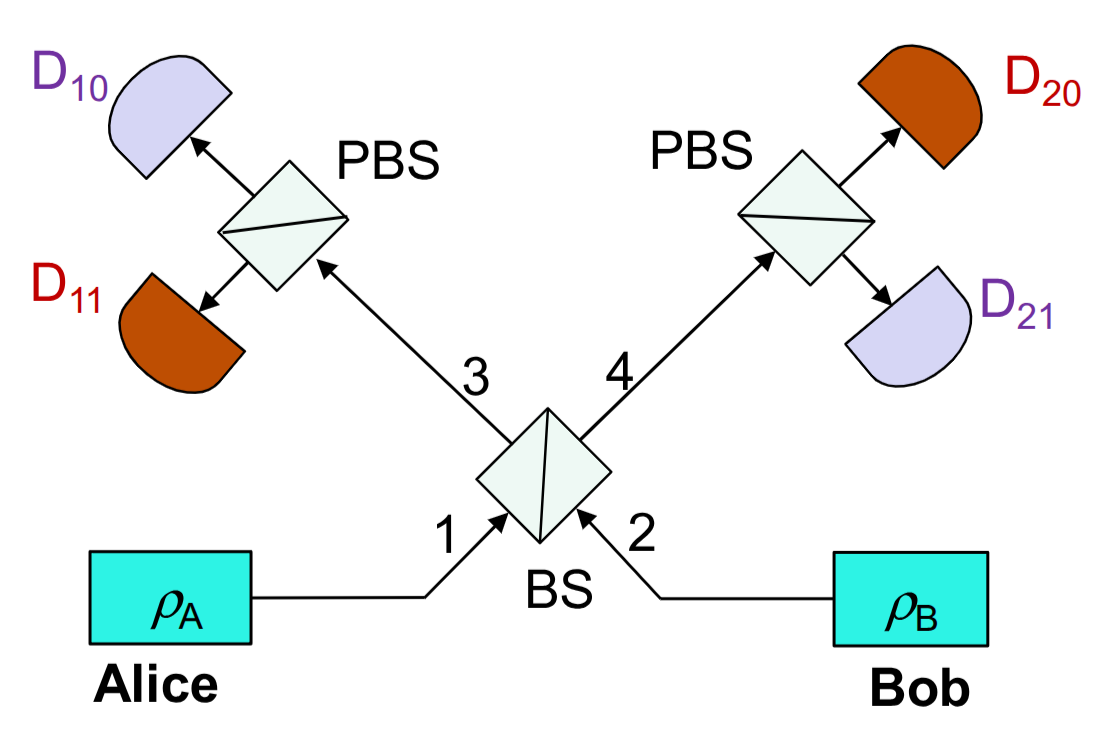
\includegraphics[width=0.8\textwidth]{chapters/figs/fig-6-12}
	\caption{تصویرسازی چیدمان برای انجام اندازه‌گیری‌های حالت بل روی حالت‌های قطبش.}
	\label{fig:6-12}
\end{figure}

از سوی دیگر، وقتی فوتون‌ها در پورت‌های ورودی یک و دوِ \lr{BS} دارای قطبش‌های متفاوتی باشند، می‌توانند از یک پورت خروجی یکسان یا پورت‌های متفاوت خارج شوند. هنگامی که هر دو فوتون از پورت خروجی ۳ خارج شوند، پس از \lr{PBS}، آشکارسازهای $D_{10}$ و $D_{11}$ به‌طور هم‌زمان کلیک می‌کنند. هنگامی که هر دو فوتون از پورت خروجی ۴ خارج شوند، پس از \lr{PBS}، آشکارسازهای $D_{20}$ و $D_{21}$ به‌طور هم‌زمان کلیک می‌کنند. زمانی که فوتون‌های ورودی با قطبش‌های متفاوت از پورت‌های متفاوتی خارج شوند، دو گزینه وجود دارد: وقتی فوتون افقی از پورت ۳ و فوتون عمودی از پورت ۴ خارج شود، $D_{11}$ و $D_{20}$ به‌طور هم‌زمان کلیک می‌کنند. در نهایت، وقتی فوتون افقی از پورت ۴ و فوتون عمودی از پورت ۳ خارج شود، $D_{10}$ و $D_{21}$ به‌طور هم‌زمان کلیک می‌کنند. با توجه به اینکه حالت‌های بل $|\psi^{\pm}\rangle$ (توسط \lr{BS}) به‌صورت زیر تبدیل می‌شوند:
\begin{equation}
	\begin{aligned}
		|\psi^+\rangle = \frac{1}{\sqrt{2}} (|01\rangle_{12} + |10\rangle_{12}) \xrightarrow{BS} |\psi_{\text{out}}^+\rangle = \frac{1}{\sqrt{2}} (|01\rangle_{33} + |10\rangle_{44}) \\
		|\psi^-\rangle = \frac{1}{\sqrt{2}} (|01\rangle_{12} - |10\rangle_{12}) \xrightarrow{BS} |\psi_{\text{out}}^-\rangle = \frac{1}{\sqrt{2}} (|01\rangle_{34} - |10\rangle_{34})
	\end{aligned}
	\label{eq:6-47}
\end{equation}
آن‌ها توسط \lr{PBS}ها و \lr{SPD}ها قابل تمایز هستند. به‌وضوح، بر اساس بحث بالا نتیجه می‌گیریم که تصویر شدن روی $|\psi^+\rangle$ زمانی رخ می‌دهد که هر دو \lr{SPD} بعد از هر یک از دو \lr{PBS} به‌طور هم‌زمان کلیک کنند. به عبارت دیگر، وقتی یا $D_{10}$ و $D_{11}$ و یا $D_{20}$ و $D_{21}$ به‌طور هم‌زمان کلیک کنند، تصویر شدن روی $|\psi^+\rangle$ شناسایی می‌شود. به‌طور مشابه، وقتی یا $D_{10}$ و $D_{21}$ و یا $D_{20}$ و $D_{11}$ به‌طور هم‌زمان کلیک کنند، تصویر شدن روی حالت $|\psi^-\rangle$ شناسایی می‌شود. در نتیجه، هنگام استفاده از \lr{SPD}های ایده‌آل، بازدهی \lr{BSM} برابر با $1/2$ است. اگر \lr{SPD}ها دارای بازدهی آشکارسازی غیرایده‌آل $\eta$ باشند، بازدهی \lr{BSM} برابر با $0.5\eta^2$ خواهد بود.

درجه آزادی دیگری که به‌طور گسترده برای کدگذاری حالت‌های کوانتومی استفاده می‌شود، درجه آزادی بازه زمانی\LTRfootnote{Time-bin} است. برای ارتباطات کوانتومی دوبعدی، فوتون را می‌توان به‌صورت برهم‌نهی از حالت زود\LTRfootnote{Early-state} (نشان‌ داده شده با $|0\rangle$) و حالت دیر\LTRfootnote{Late-state} (نشان داده شده با $|1\rangle$) به‌صورت $|\chi\rangle = a|0\rangle + b|1\rangle$ با شرط $|a|^2 + |b|^2 = 1$ کدگذاری کرد. برای انجام \lr{BSM} می‌توان از چیدمان ارائه شده در شکل \ref{fig:6-13} استفاده کرد که علاوه بر \lr{BS} تنها به دو \lr{SPD} نیاز دارد. مشابه قطبش، حالت‌های بل توسط رابطه \eqref{eq:6-45} اما با کِت‌های پایه متفاوت تعریف می‌شوند. باز هم، وقتی دو فوتون در یک زمان واحد به پورت‌های ورودی \lr{BS} می‌رسند، طبق اثر \lr{HOM} از یک پورت خروجی یکسان خارج می‌شوند و ما نمی‌توانیم حالت‌های $|\phi^{\pm}\rangle$ را متمایز کنیم. از سوی دیگر، تصویر شدن روی $|\psi^+\rangle$ زمانی شناسایی می‌شود که هر یک از آشکارسازها در بازه‌های زمانی زود و دیر کلیک ثبت کنند. به‌طور مشابه، تصویر شدن روی $|\psi^-\rangle$ زمانی رخ می‌دهد که هر یک از آشکارسازهای $D_1$ و $D_2$ یا $D_2$ و $D_1$ در بازه‌های زمانی متوالی (زود-دیر) کلیک کنند.

\begin{figure}[ht]
	\centering
	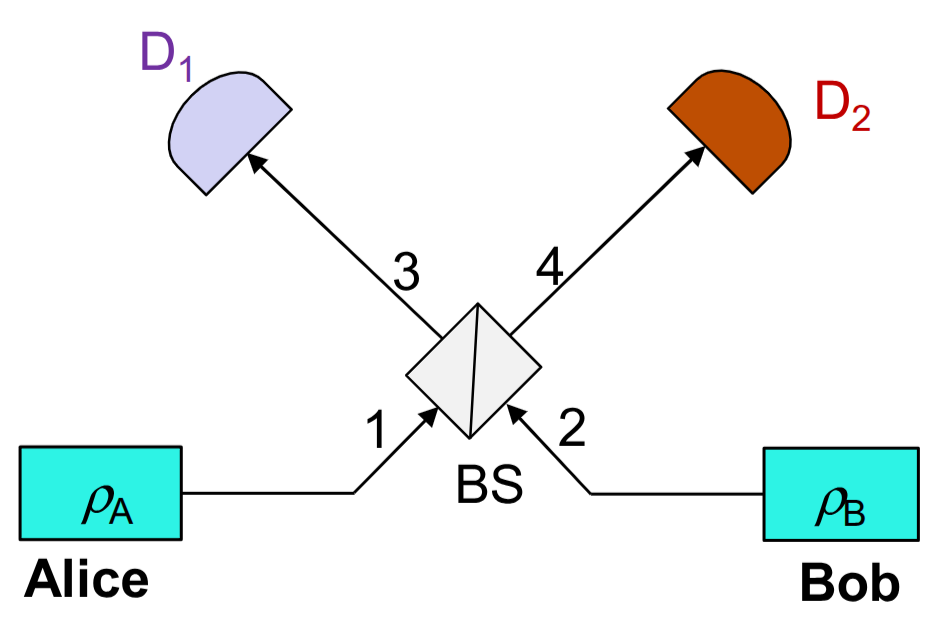
\includegraphics[width=0.8\textwidth]{chapters/figs/fig-6-13}
	\caption{تصویرسازی چیدمان برای انجام اندازه‌گیری‌های حالت بل روی حالت‌های بازه زمانی.}
	\label{fig:6-13}
\end{figure}

\subsection{شرح پروتکل توزیع کلید کوانتومی مستقل از دستگاه اندازه‌گیری}
\label{subsec:6-7-2}
در پروتکل‌های \lr{MDI-QKD} \cite{82,88,89,90,91}، آلیس و باب از طریق یک کانال کوانتومی، مانند یک پیوند نوری فضای آزاد (\lr{FSO}) یا فیبر نوری، به یک شخص ثالث به نام چارلی متصل می‌شوند. همان‌طور که در شکل \ref{fig:6-14} برای پروتکل \lr{MDI-QKD} مبتنی بر قطبش تصویر شده است، آشکارسازهای \lr{SPD} در سمت چارلی قرار دارند.

آلیس و باب می‌توانند از منابع تک‌فوتونی یا منابع \lr{WCS} استفاده کنند و به‌طور تصادفی یکی از چهار حالت $|0\rangle$، $|1\rangle$، $|+\rangle$ یا $|-\rangle$ را با کمک یک مدولاتور قطبش\LTRfootnote{Polarization modulator (PolM)} (\lr{PolM}) که بسیار شبیه به مدولاتور مورد استفاده در پروتکل \lr{BB84} است، برای ارسال به چارلی انتخاب کنند. از یک مدولاتور شدت\LTRfootnote{Intensity modulator} برای اعمال حالت‌های فریب مختلف استفاده می‌شود. چارلی اساساً می‌تواند خودِ ایو باشد. او \lr{BSM} جزئی را با کمک یک \lr{BS}، دو \lr{PBS} و چهار \lr{SPD} مطابق شکل \ref{fig:6-14} انجام می‌دهد و رویدادهایی را اعلام می‌کند که در آن‌ها نتیجه اندازه‌گیری منجر به یکی از دو حالت $|\psi^+\rangle = (|01\rangle + |10\rangle)/\sqrt{2}$ یا $|\psi^-\rangle = (|01\rangle - |10\rangle)/\sqrt{2}$ شده باشد. چارلی همچنین نتایج \lr{BSM} را فاش می‌کند. با توجه به اینکه اندازه‌گیری‌های حالت بل چارلی تنها برای بررسی توازن (پاریته) بیت‌های آلیس و باب استفاده می‌شوند، این اندازه‌گیری‌ها هیچ اطلاعاتی در مورد خودِ بیت‌های منفرد فاش نخواهند کرد \cite{88}.

\begin{figure}[ht]
	\centering
	 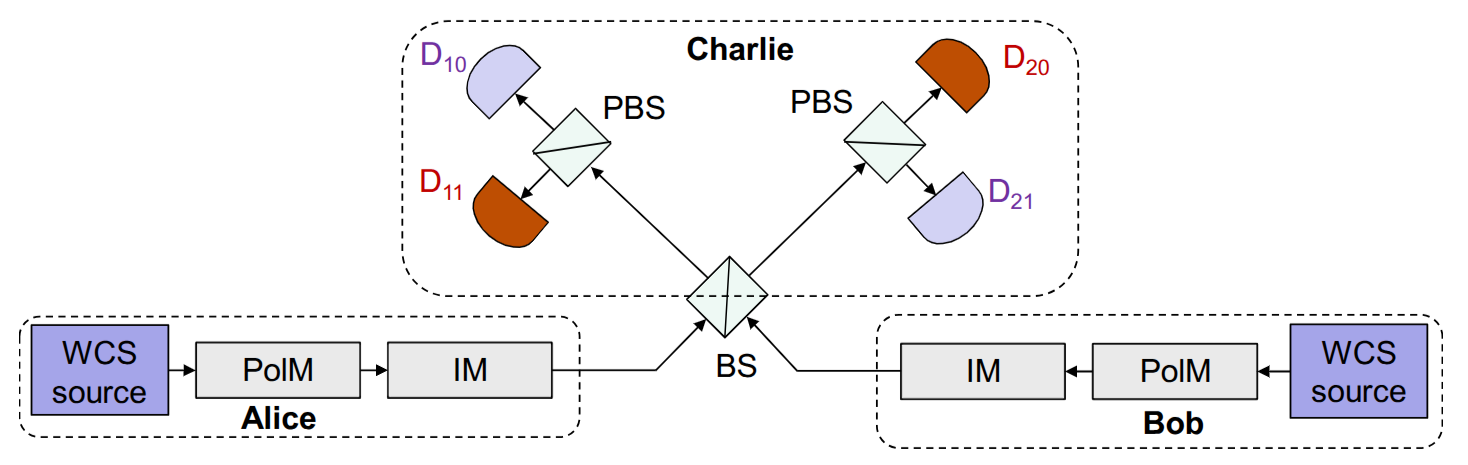
\includegraphics[width=0.8\textwidth]{chapters/figs/fig-6-14}
	\caption{پیکربندی سیستم توزیع کلید کوانتومی مستقل از دستگاه اندازه‌گیری مبتنی بر حالت قطبش.}
	\label{fig:6-14}
\end{figure}

یک \lr{BSM} موفق متناظر با مشاهداتی است که در آن دقیقاً دو آشکارساز (با قطبش‌های متعامد) به‌صورت زیر تحریک شوند:
\begin{itemize}
	\item کلیک هم‌زمان آشکارسازهای $D_{10}$ و $D_{21}$ حالت بل $|\psi^-\rangle$ را شناسایی می‌کند.
	\item از سوی دیگر، کلیک هم‌زمان آشکارسازهای $D_{11}$ و $D_{20}$ حالت بل $|\psi^+\rangle$ را شناسایی می‌کند.
\end{itemize}
سایر الگوهای آشکارسازی مربوط به حالت‌های $|\phi^{\pm}\rangle$ هستند که با \lr{SPD}ها قابل تمایز نیستند و بنابراین موفقیت‌آمیز تلقی نشده و از بررسی کنار گذاشته می‌شوند. به‌وضوح، بر اساس شرح فوق نتیجه می‌گیریم که پروتکل \lr{MDI-QKD} تعمیمی از هر دو پروتکل \lr{QKD} مبتنی بر \lr{EPR} (تبدیل شده به طرح آماده‌سازی-و-اندازه‌گیری) و پروتکل مبتنی بر حالت فریب است. آلیس و باب با مقایسه بخشی از دنباله‌های خود می‌توانند صداقت چارلی را تأیید کنند.

اکنون یک پیاده‌سازی ممکن برای \lr{PolM}، یعنی پیکربندی رمزگذار \lr{BB84} مبتنی بر حالت فریب را شرح می‌دهیم که در شکل \ref{fig:6-15} ارائه شده است. سیگنال باریکه لیزر توسط یک کوپلر ۱:۴ به چهار شاخه تقسیم می‌شود که هر شاخه شامل یک کنترل‌کننده قطبش برای اعمال حالت‌های قطبش $|0\rangle$، $|1\rangle$، $|+\rangle$ و $|-\rangle$ است. با کمک یک سوئیچ نوری فضایی\LTRfootnote{Optical space switch} ۴:۱، حالت قطبش ارسالی به چارلی را به‌طور تصادفی انتخاب می‌کنیم. برای این منظور، استفاده از سوئیچ‌هایی با سوئیچینگ الکترواپتیکی مطلوب است (مانند آنچه در مراجع \cite{92, 93} گزارش شده است)، زیرا در این سوئیچ‌ها حالت سوئیچینگ را می‌توان در عرض چند نانوثانیه تغییر داد. مدولاتور فاز در خروجی برای انجام تصادفی‌سازی فاز\LTRfootnote{Phase randomization} حالت همدوس $|\alpha\rangle = \exp(-|\alpha|^2/2) \sum \alpha^n |n\rangle / \sqrt{n!}$ به‌صورت زیر به کار می‌رود:
\begin{equation}
	\begin{aligned}
		\frac{1}{2\pi} \int_{0}^{2\pi} |\alpha e^{j\omega}\rangle \langle \alpha e^{j\omega} | d\omega &= \frac{1}{2\pi} \sum_{n=0}^{\infty} \sum_{m=0}^{\infty} \frac{|\alpha|^{m+n}}{\sqrt{m!n!}} e^{-|\alpha|^2} |n\rangle\langle m| \underbrace{\int_{0}^{2\pi} e^{j(n-m)\omega} d\omega}_{\delta_{nm}} \\
		&= \sum_{n=0}^{\infty} \frac{|\alpha|^{2n}}{n!} e^{-|\alpha|^2} |n\rangle\langle n| = \sum_{n=0}^{\infty} \frac{\mu^n}{n!} e^{-\mu} |n\rangle\langle n|; \quad \mu = |\alpha|^2
	\end{aligned}
	\label{eq:6-48}
\end{equation}
که در آن $\mu = |\alpha|^2$ میانگین تعداد فوتون در هر پالس است. سپس از یک تضعیف‌کننده نوری متغیر برای کاهش میانگین تعداد فوتون تا سطح کوانتومی استفاده می‌شود. سایر پیکربندی‌های \lr{PolM} نیز می‌توانند استفاده شوند، مانند آنچه در مرجع \cite{88} با استفاده از چهار دیود لیزری شرح داده شده است. آلیس و باب سپس از طریق یک کانال کلاسیک احرازهویت‌شده و بدون نویز، اطلاعات مربوط به پایه‌های استفاده شده را مبادله می‌کنند: پایه $Z$ شامل حالت‌های $|0\rangle$ و $|1\rangle$ (پایه محاسباتی) یا پایه $X$ شامل حالت‌های $|+\rangle$ و $|-\rangle$ (پایه قطری). پس از آن، آلیس و باب تنها رویدادهایی را نگه می‌دارند که در آن‌ها از پایه یکسانی استفاده کرده‌اند و در عین حال چارلی حالت‌های \lr{BSM} یعنی $|\psi^-\rangle$ یا $|\psi^+\rangle$ را اعلام کرده است. یکی از آن‌ها (مثلاً باب) بیت‌های ارسالی را وارونه (فلیپ) می‌کند، مگر زمانی که هر دو از پایه قطری استفاده کرده باشند و چارلی حالت $|\psi^+\rangle$ را اعلام کرده باشد. سایر رویدادها کنار گذاشته می‌شوند.

\begin{figure}[ht]
	\centering
	 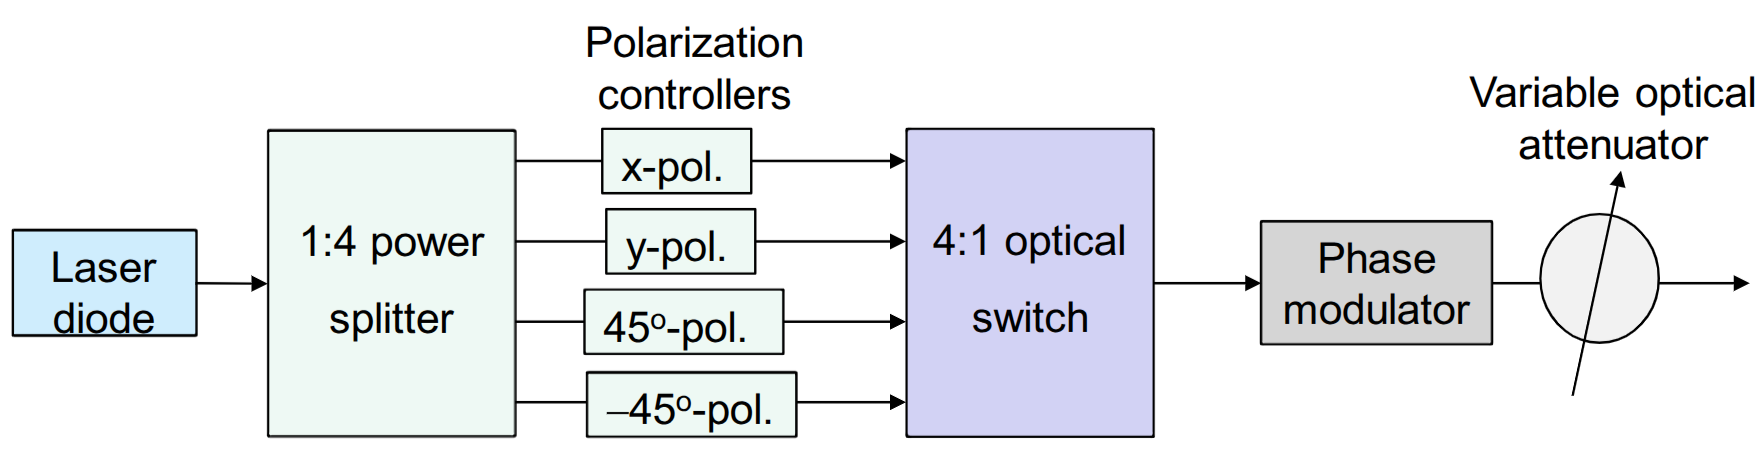
\includegraphics[width=0.8\textwidth]{chapters/figs/fig-6-15}
	\caption{پیکربندی رمزگذار \lr{BB84} (\lr{PolM}) مبتنی بر حالت فریب.}
	\label{fig:6-15}
\end{figure}





علاوه بر این، کلید-$X$ از آن بیت‌هایی تشکیل می‌شود که آلیس و باب فوتون‌های خود را در پایه $X$ (پایه قطری) آماده کرده بودند. نرخ خطا در این بیت‌ها برای محدود کردن اطلاعات کسب شده توسط ایو استفاده می‌شود. سپس، آلیس و باب کلید-$Z$ را از آن بیت‌هایی تشکیل می‌دهند که برای آن‌ها هر دو از پایه $Z$ (پایه محاسباتی) استفاده کرده‌اند. در نهایت، آن‌ها مصالحه اطلاعات و تقویت حریم خصوصی را روی کلید-$Z$ انجام می‌دهند تا به کلید مخفی دست یابند.

پروتکل \lr{MDI-QKD} علاوه بر حساس نبودن به \lr{SPD}های استفاده شده توسط چارلی، امکان اتصال چندین شرکت‌کننده را در یک شبکه \lr{QKD} ستاره‌ای\LTRfootnote{Star-like QKD network} فراهم می‌کند که در آن چارلی در مرکز (به‌عنوان یک هاب\LTRfootnote{Hub}) قرار دارد \cite{94, 95}. در این شبکه \lr{QKD} که در شکل \ref{fig:6-16} نشان داده شده است، گران‌ترین تجهیزات (\lr{SPD}ها) بین چندین کاربر به اشتراک گذاشته می‌شوند و شبکه \lr{QKD} را می‌توان به راحتی و بدون ایجاد اختلال برای سایر کاربران ارتقا داد. با کمک یک سوئیچ نوری $N:2$، هر دو کاربر می‌توانند در پروتکل \lr{MDI-QKD} برای تبادل کلیدهای امن شرکت کنند.

\begin{figure}[ht]
	\centering
	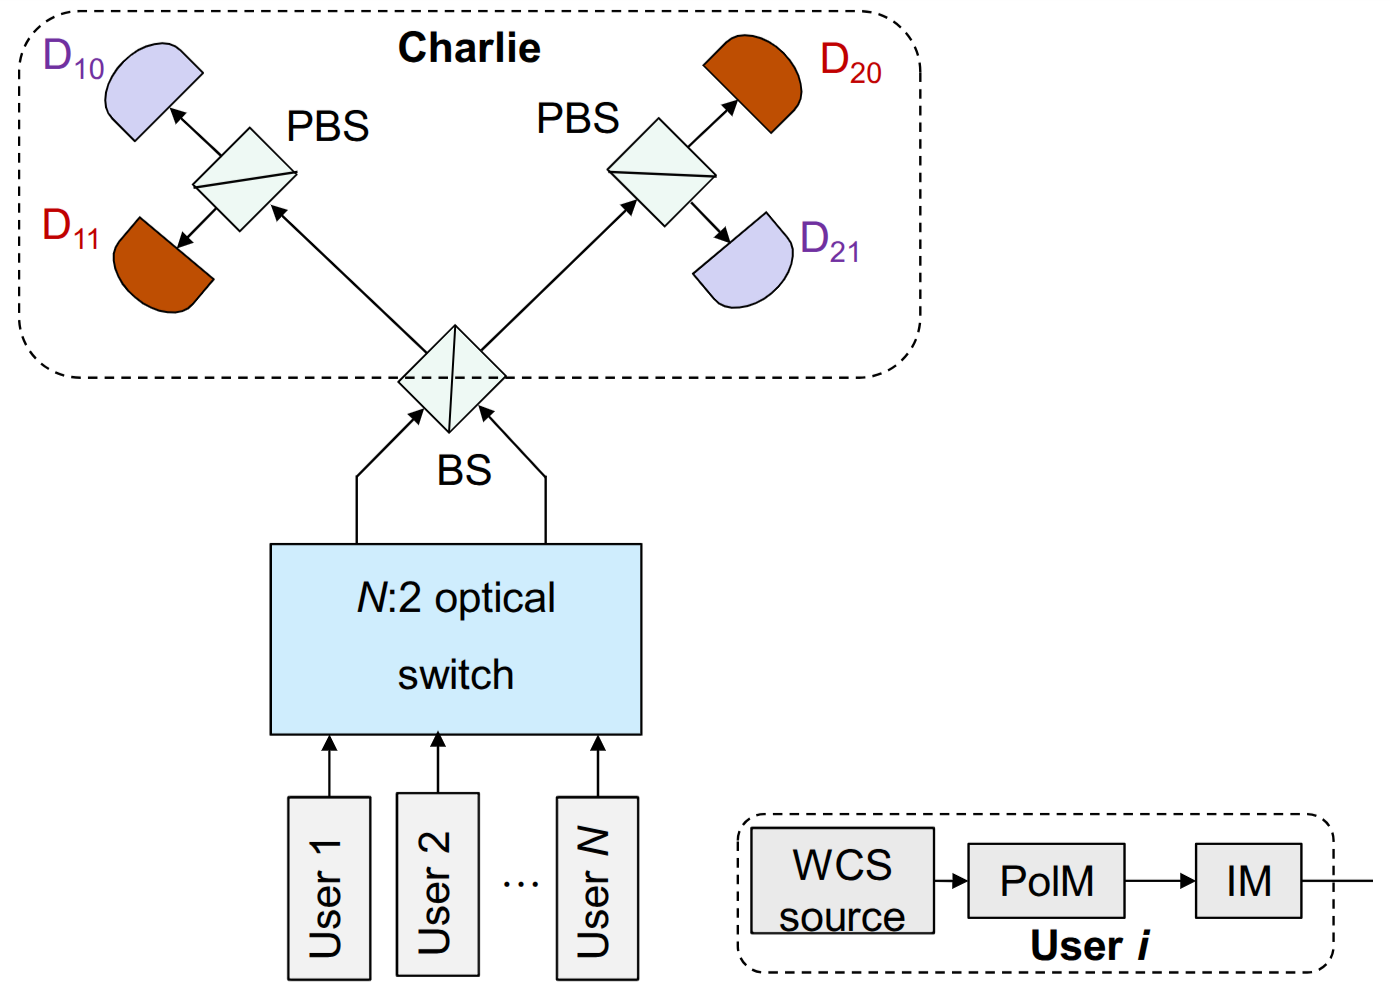
\includegraphics[width=0.7\textwidth]{chapters/figs/fig-6-16}
	\caption{پیکربندی شبکه توزیع کلید کوانتومی ستاره‌ای مبتنی بر \lr{MDI-QKD}.}
	\label{fig:6-16}
\end{figure}

\subsubsection{پروتکل توزیع کلید کوانتومی مستقل از دستگاه اندازه‌گیری مبتنی بر کدگذاری فاز-زمان}
\label{subsec:6-7-3}
حالت‌های پایه کدگذاری فاز-زمان برای پروتکل \lr{BB84} ($N=2$) در شکل \ref{fig:6-17} ارائه شده‌اند. پایه زمانی متناظر با پایه محاسباتی $\{|0\rangle, |1\rangle\}$ است، در حالی که پایه فازی متناظر با پایه قطری $\{|+\rangle, |-\rangle\}$ می‌باشد. پالس در یک بازه زمانی\LTRfootnote{Time bin} با مدت‌زمان $\tau = T/2$ متمرکز شده است. پایه زمانی مشابه \lr{PPM} است. حالتی که در آن فوتون در اولین بازه زمانی قرار می‌گیرد (حالت زود\LTRfootnote{Early state})، با $|0\rangle = |e\rangle$ نشان داده می‌شود، در حالی که حالتی که در آن فوتون در دومین بازه زمانی قرار می‌گیرد (حالت دیر\LTRfootnote{Late state})، با $|1\rangle = |l\rangle$ نشان داده می‌شود. حالت‌های فاز-زمان به‌صورت $|+\rangle = (|0\rangle + |1\rangle)/\sqrt{2}$ و $|-\rangle = (|0\rangle - |1\rangle)/\sqrt{2}$ تعریف می‌شوند. آلیس به‌طور تصادفی یا پایه زمانی یا پایه فازی را انتخاب کرده و متعاقب آن به‌طور تصادفی حالت پایه را انتخاب می‌کند. مقدار منطقی $0$ توسط $|0\rangle$ و $|+\rangle$ بازنمایی می‌شود؛ در حالی که مقدار منطقی $1$ توسط $|1\rangle$ و $|-\rangle$ نشان داده می‌شود. آلیس و باب به‌طور تصادفی یکی از چهار حالت $|0\rangle, |1\rangle, |+\rangle, |-\rangle$ را برای ارسال به چارلی انتخاب می‌کنند. چارلی \lr{BSM} جزئی را با کمک یک \lr{BS} ۵۰:۵۰ و دو \lr{SPD} مطابق شکل \ref{fig:6-18} انجام می‌دهد و رویدادهایی را اعلام می‌کند که در آن‌ها نتیجه اندازه‌گیری منجر به یکی از دو حالت $|\psi^+\rangle = (|01\rangle + |10\rangle)/\sqrt{2}$ یا $|\psi^-\rangle = (|01\rangle - |10\rangle)/\sqrt{2}$ شده باشد.



\begin{figure}[ht]
	\centering
	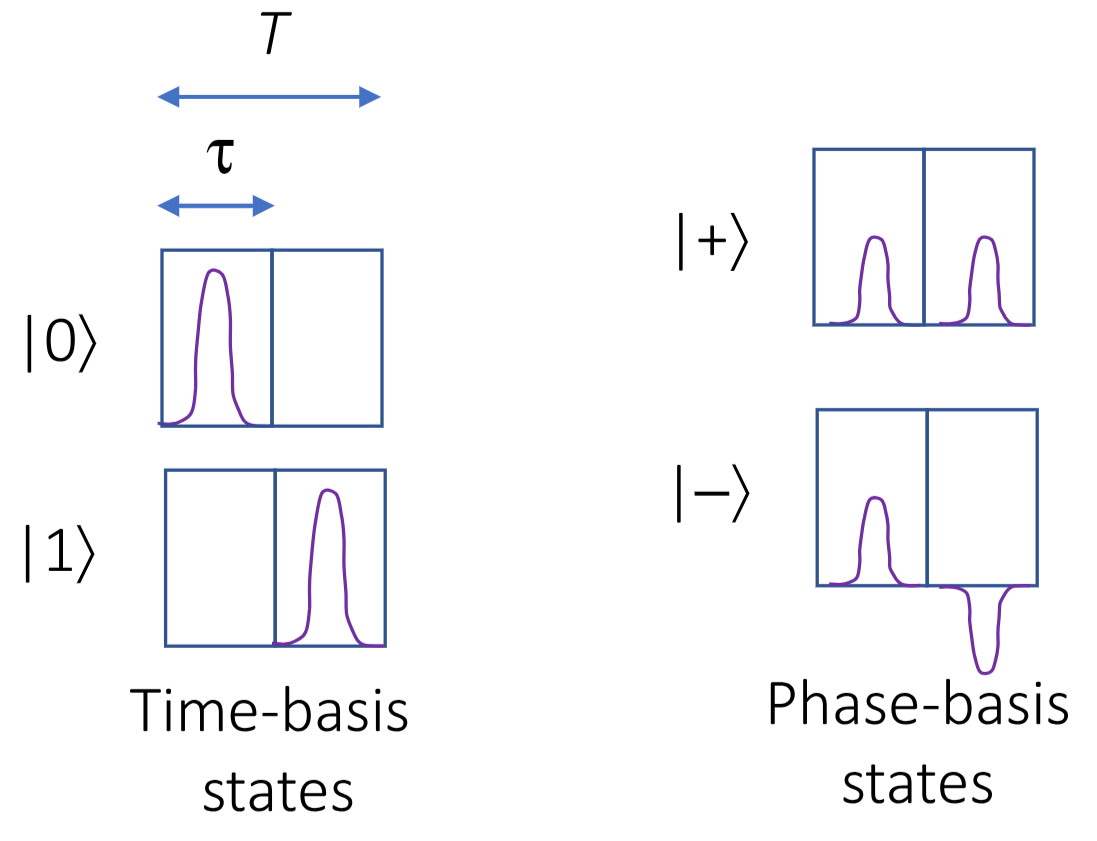
\includegraphics[width=0.5\textwidth]{chapters/figs/fig-6-17}
	\caption{حالت‌های پایه زمانی و پایه فازی مورد استفاده در کدگذاری فاز-زمان برای پروتکل \lr{BB84}.}
	\label{fig:6-17}
\end{figure}

چارلی همچنین نتیجه \lr{BSM} را فاش می‌کند. یک \lr{BSM} موفق متناظر با مشاهداتی است که در آن‌ها \lr{SPD}ها به‌صورت زیر تحریک شوند:
\begin{itemize}
	\item دو کلیک متوالی (هر دو در بازه‌های زمانی زود و دیر) روی یکی از \lr{SPD}ها، حالت بل $|\psi^-\rangle$ را شناسایی می‌کند.
	\item از سوی دیگر، زمانی که یک \lr{SPD} حضور فوتون را در بازه زمانی زود و دیگری در بازه زمانی دیر آشکار کند، حالت بل $|\psi^+\rangle$ را شناسایی می‌کنیم.
	\item سایر الگوهای آشکارسازی مربوط به حالت‌های $|\phi^{\pm}\rangle$ هستند و از بررسی کنار گذاشته می‌شوند.
\end{itemize}
بقیه پروتکل مشابه پروتکل \lr{MDI-QKD} مبتنی بر حالت قطبش است. برای پیاده‌سازی رمزگذار فاز-زمان، آلیس و باب می‌توانند یا از مدولاتور قطبی الکترواپتیکی، متشکل از اتصال پیاپی یک مدولاتور دامنه و یک مدولاتور فاز (مطابق شکل \ref{fig:6-18}) استفاده کنند، و یا به‌صورت جایگزین، یک مدولاتور \lr{I/Q} الکترواپتیکی را به کار گیرند \cite{46, 96}. مدولاتور دامنه (مدولاتور ماخ-زندر) برای شکل‌دهی پالس و مدولاتور فاز برای اعمال جابه‌جایی فاز مطلوب مطابق با حالت‌های پایه فازی استفاده می‌شود (شکل \ref{fig:6-17} را ببینید). از \lr{AWG}ها می‌توان برای تولید شکل‌موج‌های \lr{RF} متناظر بر حسب نیاز استفاده کرد. \lr{VOA}ها نیز برای تضعیف باریکه مدوله‌شده تا سطح تک‌فوتون به کار می‌روند. برای عملکرد صحیح، \lr{AWG}ها باید هم‌زمان\LTRfootnote{Synchronized} باشند. علاوه بر این، دیودهای لیزر موج پیوسته\LTRfootnote{Continuous-wave (CW)} مورد استفاده توسط آلیس و باب باید قفل فرکانسی\LTRfootnote{Frequency locked} شده باشند. در نهایت، فوتون‌های ورودی به \lr{BSM} (از سوی آلیس و باب) باید قطبش یکسانی داشته باشند.

\begin{figure}[ht]
	\centering
	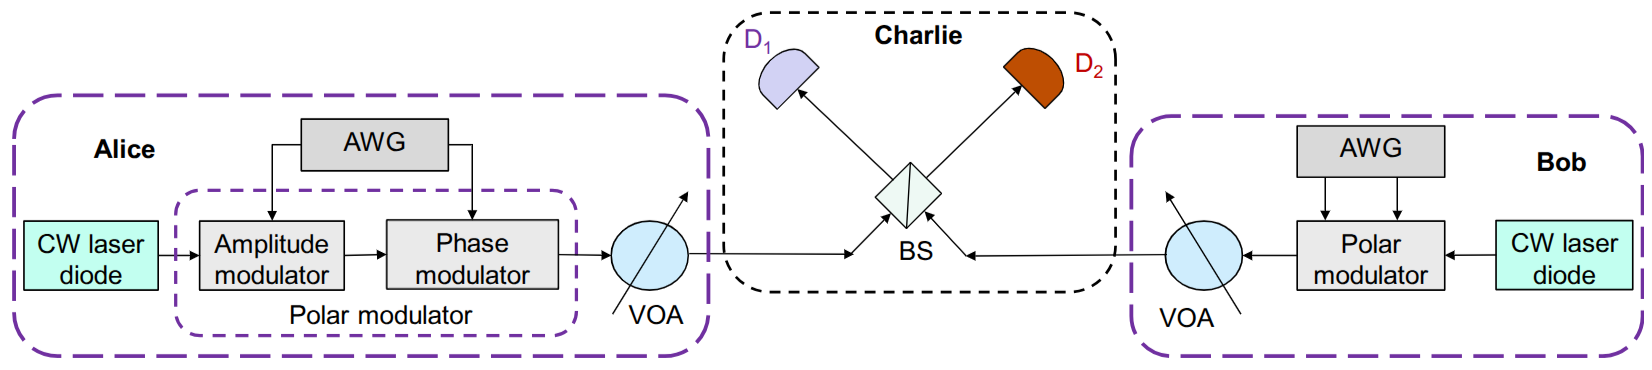
\includegraphics[width=\textwidth]{chapters/figs/fig-6-18}
	\caption{پیکربندی سیستم توزیع کلید کوانتومی مستقل از دستگاه اندازه‌گیری مبتنی بر کدگذاری فاز-زمان.}
	\label{fig:6-18}
\end{figure}

\subsubsection{کسر امنیت پروتکل‌های توزیع کلید کوانتومی مستقل از دستگاه اندازه‌گیری}
\label{subsec:6-7-4}
کسر مخفی پروتکل \lr{MDI-QKD}، زمانی که آلیس و باب هر دو از منابع تک‌فوتونی استفاده می‌کنند، مشابه پروتکل \lr{BB84} است:
\begin{equation}
	r = q(Z) [ 1 - h_2(e(X)) ] - q(Z) f_e h_2(e(Z))
	\label{eq:6-49}
\end{equation}
که در آن $q(Z)$ اکنون نشان‌دهنده احتمال نتیجه موفقیت‌آمیز \lr{BSM} («بهره») است. از سوی دیگر، زمانی که آلیس و باب هر دو از منابع \lr{WCS} استفاده می‌کنند، باید روش حالت فریب به کار گرفته شود تا کسر مخفی مطابق مرجع \cite{89} به‌صورت زیر تخمین زده شود:
\begin{equation}
	r = q(Z)_{11} [ 1 - h_2(e(X)_{11}) ] - q(Z)_{\mu\sigma} f_e h_2(e(Z)_{\mu\sigma})
	\label{eq:6-50}
\end{equation}
که در آن نمادگذاری‌های زیر را معرفی کردیم:
\begin{itemize}
	\item $q(Z)_{11}$ نشان‌دهنده احتمالی است که چارلی یک نتیجه موفقیت‌آمیز («بهره») را اعلام کند، در حالی که آلیس و باب هر کدام یک تک‌فوتون را در پایه $Z$ ارسال کرده‌اند.
	\item $e(X)_{11}$ نشان‌دهنده نرخ خطای فاز سیگنال‌های تک‌فوتونی است که هر دو در پایه $Z$ ارسال شده‌اند.
	\item $q(Z)_{\mu\sigma}$ نشان‌دهنده بهره در پایه $Z$ است، زمانی که آلیس حالت \lr{WCS} با شدت $\mu$ را برای چارلی ارسال می‌کند، در حالی که باب به‌طور هم‌زمان حالت \lr{WCS} با شدت $\sigma$ را می‌فرستد.
\end{itemize}
در معادله فوق، اطلاعات حذف شده از کلید نهایی در مرحله تقویت حریم خصوصی توسط جمله $q(Z)_{11} h_2(e(X)_{11})$ توصیف می‌شود. اطلاعات فاش شده توسط آلیس در مرحله مصالحه اطلاعات با جمله $q(Z)_{\mu\sigma} f_e h_2(e(Z)_{\mu\sigma})$ توصیف می‌گردد که در آن مانند قبل، $f_e$ ناکارآمدی تصحیح خطا ($f_e \geq 1$) است. نرخ‌های خطای $q(Z)_{11}$ و $e(X)_{11}$ را نمی‌توان به‌طور مستقیم اندازه‌گیری کرد، بلکه در عوض با به‌کارگیری رویکرد حالت فریب به شیوه‌ای مشابه آنچه در بخش قبل شرح داده شد، محدود می‌شوند.


\section{پروتکل‌های توزیع کلید کوانتومی میدان-دوقلو}
\label{sec:6-8}
کانال کوانتومی را می‌توان با گذردهی\LTRfootnote{Transmissivity} $T$ مشخص کرد که می‌توان آن را به عنوان احتمال ارسال موفقیت‌آمیز یک فوتون توسط کانال نیز تفسیر کرد. ظرفیت کلید-مخفی کانال کوانتومی می‌تواند به عنوان حد بالایی برای حداکثر نرخ کلید مخفی ممکن استفاده شود. در بسیاری از موارد، کران پیراندولا-لورنزا-اوتاویانی-بانکی\LTRfootnote{Pirandola-Laurenza-Ottaviani-Banchi (PLOB)} (\lr{PLOB}) روی نرخ کلید خطی استفاده می‌شود که طبق مرجع \cite{97} به‌صورت $r_{PLOB} = -\log_2(1-T)$ داده می‌شود. برای غلبه بر محدودیت نرخ-مسافت در پروتکل‌های \lr{DV-QKD}، تا همین اواخر دو رویکرد دنبال شده است: (الف) توسعه رله‌های کوانتومی\LTRfootnote{Quantum relays} \cite{98} و (ب) استفاده از رله‌های مورد اعتماد\LTRfootnote{Trusted relays} \cite{99}. متأسفانه، رله‌های کوانتومی نیازمند استفاده از حافظه‌های کوانتومی با زمان طولانی و تقطیر درهم‌تنیدگی\LTRfootnote{Entanglement distillation} با وفاداری بالا هستند که هنوز با فناوری فعلی دور از دسترس می‌باشند. از سوی دیگر، روش رله مورد اعتماد فرض می‌کند که رله بین دو کاربر قابل اعتماد است و تأیید این فرض در عمل دشوار است. رویکرد \lr{MDI-QKD} که در بخش قبل شرح داده شد، توانست گریزگاه‌های آشکارسازی\LTRfootnote{Detection loopholes} را ببندد و مسافت ارسال را افزایش دهد؛ با این حال، \lr{SKR} آن همچنان توسط وابستگی $O(T)$ در حد بالا محدود می‌شود.

اخیراً، \lr{QKD} میدان-دوقلو\LTRfootnote{Twin-field QKD (TF-QKD)} (\lr{TF-QKD}) برای غلبه بر محدودیت نرخ-مسافت پیشنهاد شده است \cite{100}. نویسندگان در مرجع \cite{100} نشان داده‌اند که حد بالای \lr{TF-QKD} با ریشه دوم گذردهی مقیاس‌بندی می‌شود، یعنی $r \approx O(\sqrt{T})$. در \lr{TF-QKD}، آلیس و باب یک جفت میدان نوری با فازهای تصادفی و کدگذاری فاز در پایه‌های $X$ و $Y$ در مقاصد دور تولید کرده و آن‌ها را برای چارلی (یا ایو) غیرقابل‌اعتماد ارسال می‌کنند که او سپس آشکارسازی تک‌فوتون را انجام می‌دهد. این طرح مزایای طرح \lr{MDI-QKD} مانند مصونیت در برابر حملات آشکارساز، تسهیم‌سازی\LTRfootnote{Multiplexing} \lr{SPD} و معماری شبکه ستاره‌ای را حفظ کرده و در عین حال بر کران \lr{PLOB} غلبه می‌کند. اثبات امنیت غیرمشروط در مرجع \cite{100} ارائه نشده بود، اما در مجموعه‌ای از مقالات ثابت شد که این طرح از امنیت غیرمشروط برخوردار است \cite{101,102,103,104}. طرح \lr{TF-QKD} را می‌توان به عنوان تعمیمی از هر دو مورد (۱) طرح \lr{MDI-QKD} مبتنی بر کدگذاری فاز-زمان نشان داده شده در شکل \ref{fig:6-18} و (۲) \lr{BB84} مبتنی بر کدگذاری فاز (بخش \ref{sec:6-4-4}) تفسیر کرد.

نویسندگان در مرجع \cite{104} نشان داده‌اند که طرح \lr{TF-QKD} را می‌توان به عنوان یک طرح \lr{MDI-QKD} خاص که در یک زیرفضای دوبعدی از حالت خلاء $|0\rangle$ و حالت تک‌فوتونی $|1\rangle$ پیاده‌سازی شده است تفسیر کرد (همان‌طور که در شکل \ref{fig:6-19} نشان داده شده است) که نشان‌دهنده یک مدل معادل برای \lr{TF-QKD} با منابع تک‌فوتونی و دیودهای لیزری است. با توجه به اینکه حالت خلاء نسبت به تلفات کانال حساس نیست، این حالت همیشه قابل آشکارسازی است، یعنی «عدم کلیک» به معنای آشکارسازی موفقیت‌آمیز حالت خلاء است. این بهبود در احتمال آشکارسازی حالت خلاء عملاً منجر به \lr{SKR} بالاتری نسبت به \lr{MDI-QKD} سنتی شده و کران نرخ کلید خطی را می‌شکند. پایه محاسباتی یا پایه $Z$ توسط $\{|0\rangle, |1\rangle\}$ تعریف می‌شود (که در آن $|0\rangle$ و $|1\rangle$ همان‌طور که در بالا ذکر شد، به‌ترتیب نشان‌دهنده حالت خلاء و تک‌فوتونی هستند). پایه $X$ (پایه قطری) توسط $\{ |+\rangle = (|0\rangle + |1\rangle)/\sqrt{2}, |-\rangle = (|0\rangle - |1\rangle)/\sqrt{2} \}$ تعریف می‌شود، در حالی که پایه $Y$ توسط $\{ |+j\rangle = (|0\rangle + j|1\rangle)/\sqrt{2}, |-j\rangle = (|0\rangle - j|1\rangle)/\sqrt{2} \}$ تعریف می‌گردد. حالت‌های بل نیز به شیوه‌ای مشابه قبل تعریف می‌شوند، یعنی $|\psi^{\pm}\rangle = (|01\rangle \pm |10\rangle)/\sqrt{2}$.

آلیس (باب) با کمک دومین سوئیچ نوری به‌طور تصادفی انتخاب می‌کند که از پایه $Z$ یا پایه $X/Y$ استفاده کند. وقتی پایه $Z$ انتخاب می‌شود، آلیس (باب) سوئیچ نوری اول را برای انتخاب تصادفی حالت خلاء $|0\rangle$ یا حالت تک‌فوتونی به کار می‌گیرد و حالت انتخاب شده از طریق یک کانال نوری (فیبر \lr{SMF} یا پیوند \lr{FSO}) به سمت چارلی ارسال می‌شود. وقتی شاخه پایه $X/Y$ انتخاب می‌شود، لیزر \lr{CW} حالت همدوس $|\alpha\rangle$ را تولید می‌کند که توسط \lr{VOA} تضعیف می‌شود تا حالت برهم‌نهی از خلاء و تک‌فوتون به‌دست آید، یعنی $|+\rangle = (|0\rangle + |1\rangle)/\sqrt{2}$. آلیس (باب) با کمک یک مدولاتور فاز به‌طور تصادفی یکی از چهار فاز را از مجموعه $\{0, \pi, \pi/2, 3\pi/2\}$ انتخاب می‌کند. به این ترتیب، هر دو حالت برای پایه $X$ و پایه $Y$ به‌صورت تصادفی انتخاب می‌شوند. (به‌صورت جایگزین، به جای دو سوئیچ نوری ۲:۱، می‌توان از یک سوئیچ نوری ۴:۱ استفاده کرد).

\begin{figure}[ht]
	\centering
	 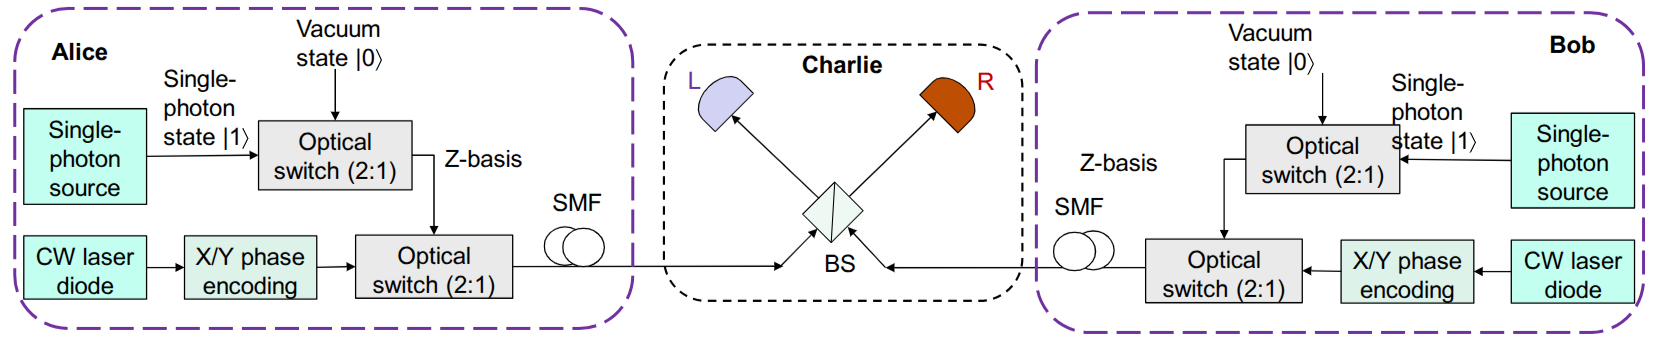
\includegraphics[width=\textwidth]{chapters/figs/fig-6-19}
	\caption{سیستم مفهومی توزیع کلید کوانتومی میدان-دوقلو با منابع تک‌فوتونی و لیزر موج پیوسته.}
	\label{fig:6-19}
\end{figure}

چارلی اندازه‌گیری‌های \lr{BSM} را انجام می‌دهد. آشکارسازی هم‌زمانی با کلیک \lr{SPD} سمت راست ($R$) و عدم کلیک در \lr{SPD} سمت چپ ($L$) نشان‌دهنده حالت بل $|\psi^-\rangle$ است. از سوی دیگر، آشکارسازی هم‌زمانی با کلیک \lr{SPD} سمت چپ و عدم کلیک در \lr{SPD} سمت راست نشان‌دهنده حالت بل $|\psi^+\rangle$ است. سپس آلیس و باب پایه استفاده شده را از طریق یک کانال عمومی احرازهویت‌شده مبادله می‌کنند. باب زمانی که از پایه $Z$ استفاده شده باشد و چارلی حالت‌های بل $|\psi^-\rangle$ را شناسایی کند، دنباله خود را وارونه (فلیپ) می‌کند. همچنین باب زمانی که از پایه $X$ یا $Y$ استفاده شده باشد و چارلی حالت بل $|\psi^-\rangle$ را شناسایی کند، دنباله خود را وارونه خواهد کرد. پس از اتمام فرآیند غربال‌گری، آلیس و باب از دنباله‌های مربوط به پایه $Z$ برای کلید استفاده خواهند کرد، در حالی که دنباله‌های مربوط به پایه $X/Y$ برای تخمین نرخ خطای بیت کوانتومی استفاده می‌شوند. در نهایت، آلیس و باب مراحل پس‌پردازش کلاسیک، مصالحه اطلاعات و تقویت حریم خصوصی را برای دستیابی به کلید امن مشترک انجام می‌دهند.

اکنون توجه خود را به طرح کاربردی‌تر و واقع‌گرایانه‌تر \lr{TF-QKD} نشان داده شده در شکل \ref{fig:6-20} معطوف می‌کنیم که نیازی به استفاده از منابع تک‌فوتونی ندارد. برای توضیح این طرح، از تفسیری مشابه مرجع \cite{104} استفاده می‌کنیم. هر دو آلیس و باب از لیزرهای \lr{CW} پایدار شده با پهنای خط کم برای تولید پالس‌های نوری با فاز سراسری پایدار شده با کمک یک مدولاتور دامنه استفاده می‌کنند. با کمک مدولاتورهای فاز، آلیس و باب فازهای تصادفی $\phi_A \in [0, 2\pi]$ و $\phi_B \in [0, 2\pi]$ را انتخاب می‌کنند. اختلاف فازهای تصادفی بین آلیس و باب به‌صورت گسسته در می‌آیند به‌طوری که:
\begin{equation}
	\Delta\phi_{A,B} \in \left[ \frac{2\pi}{M}k_{A,B}, \frac{2\pi}{M}(k_{A,B} + 1) \right)
	\label{eq:6-51}
\end{equation}
که در آن بازه فازی\LTRfootnote{Phase-bin} توسط $k_{A,B} \in \{0, 1, \dots, M-1\}$ گسسته‌سازی می‌شود. سپس آلیس (باب) به‌طور تصادفی انتخاب می‌کند که از پایه $Z$ یا پایه $X/Y$ استفاده کند. وقتی پایه $Z$ انتخاب می‌شود، حالت همدوس با فاز تصادفی با شدت $\mu$ یا $0$ ارسال می‌شود که به‌ترتیب نشان‌دهنده بیت‌های منطقی ۱ و ۰ با احتمال $t$ و $1-t$ است. برای کانال با تلفات، حالت میدان-دوقلو $|1\rangle_A |1\rangle_B$ می‌تواند آشکارسازی حالت بل را با خطا ایجاد کند، بنابراین بیت‌های منطقی ۰ و ۱ با احتمال یکسان ارسال نمی‌شوند بلکه با احتمالات بهینه شده ارسال می‌گردند. وقتی کدگذاری پایه $X(Y)$ انتخاب می‌شود، آلیس و باب از مدولاتورهای فاز و دامنه متناظر برای انتخاب تصادفی $0$ ($\pi/2$) و $\pi$ ($3\pi/2$) استفاده می‌کنند که نشان‌دهنده بیت‌های منطقی ۰ و ۱ است و این پالس‌های کدگذاری شده فازی با شدت‌های انتخاب شده تصادفی $\{ \nu/2, \omega/2, 0 \}$ ارسال می‌شوند. حالت‌های کوانتومی متناظر تولید شده توسط آلیس و باب از طریق پیوند نوری (\lr{SMF} یا \lr{FSO}) به سمت چارلی ارسال می‌شوند. کنترل‌کننده‌های قطبش اطمینان حاصل می‌کنند که پالس‌های آلیس و باب دارای قطبش یکسانی هستند. چارلی \lr{BSM} را انجام داده و نتایج را به همان شیوه‌ای که در بالا شرح داده شد اعلام می‌کند. سپس آلیس و باب اطلاعات فاز خود یعنی $k_{A,B}$ و شدت‌ها را که برای تخمین پارامتر استفاده می‌شوند، فاش می‌کنند. آن‌ها اطلاعات مربوط به پایه $Z$ را نسبت به چارلی محرمانه نگه می‌دارند و این داده‌ها برای کلید خام استفاده می‌شوند. سپس آلیس و باب مراحل پس‌پردازش کلاسیک، مصالحه اطلاعات و تقویت حریم خصوصی را برای دستیابی به کلید امن مشترک انجام می‌دهند.

\begin{figure}[ht]
	\centering
	 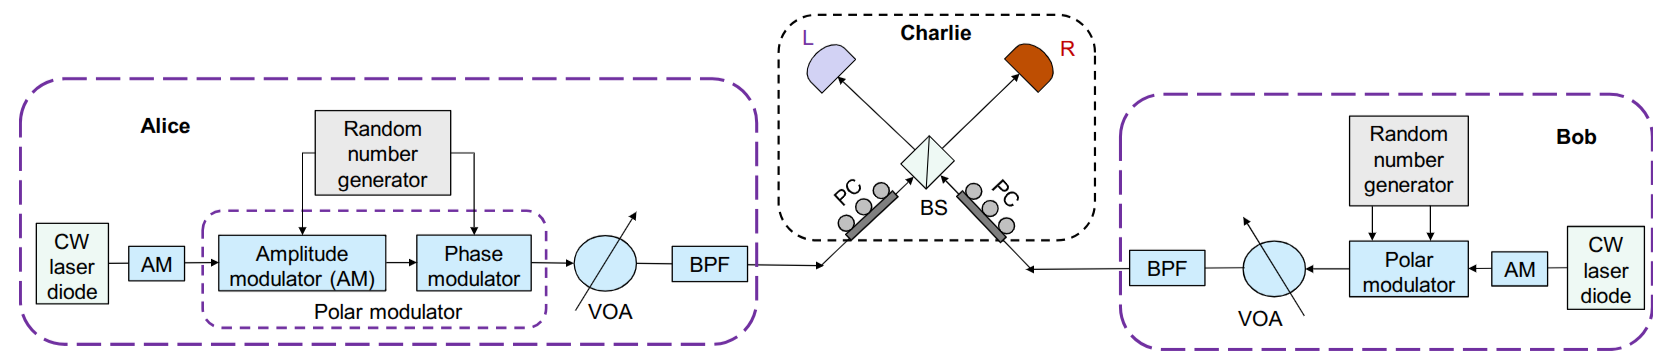
\includegraphics[width=\textwidth]{chapters/figs/fig-6-20}
	\caption{پیکربندی سیستم کاربردی توزیع کلید کوانتومی میدان-دوقلو. \lr{BPF}: فیلتر میان‌گذر نوری؛ \lr{PC}: کنترل‌کننده قطبش.}
	\label{fig:6-20}
\end{figure}

برای پروتکل \lr{BB84} مبتنی بر \lr{TF}، آلیس و باب داده‌های خام را برای کدگذاری فاز تنها در صورتی نگه می‌دارند که $|k_A - k_B| = 0$ یا $M/2$ باشد (زمانی که هر دو از پایه $X$ استفاده کرده‌اند) و سایر نتایج داده‌های خام حذف می‌شوند. برای $|k_A - k_B| = 0$، زمانی که چارلی حالت بل $|\psi^-\rangle$ را آشکار می‌کند، باب بیت کلید خود را وارونه می‌کند. به‌طور مشابه، برای $|k_A - k_B| = M/2$، زمانی که چارلی حالت بل $|\psi^+\rangle$ را آشکار می‌کند، باب بیت کلید خود را وارونه می‌کند. کسر مخفی برای پروتکل \lr{BB84} مبتنی بر \lr{TF} را می‌توان طبق مرجع \cite{104} به‌صورت زیر تخمین زد:
\begin{equation}
	\begin{aligned}
		Q_{ZZ} &= 2p_d(1-p_d)(1-t)^2 + 4(1-p_d)e^{-\mu T_{tot}/2} [1-(1-p_d)e^{-\mu T_{tot}/2}]t(1-t) \\
		&\quad + [2(1-p_d)e^{-\mu T_{tot}} I_0(\mu T_{tot}) - (1-p_d)e^{-\mu T_{tot}}]t^2 \\
		E_{ZZ} &= \frac{2p_d(1-p_d)(1-t)^2 + 2(1-p_d)e^{-\mu T_{tot}} I_0(\mu T_{tot}) - (1-p_d)e^{-\mu T_{tot}} t^2}{Q_{ZZ}}
	\end{aligned}
	\label{eq:6-53}
\end{equation}
که در آن $T_{tot} = T\eta_d$ است، به‌طوری‌که $T$ گذردهی و $\eta_d$ بازدهی آشکارساز\LTRfootnote{Detector efficiency} می‌باشد. پارامتر $p_d$ نشان‌دهنده نرخ جریان تاریک\LTRfootnote{Dark current rate} آشکارساز آستانه‌ای است. بر اساس روابط \eqref{eq:6-34} و \eqref{eq:6-35}، با قرار دادن $\mu = \nu/2$، $\sigma_1 = \omega/2$ و $\sigma_2 = 0$، کران پایین بازده $y_{1ZZ}^{(TF)}$ طبق مرجع \cite{2} به‌صورت زیر به‌دست می‌آید:
\begin{equation}
	y_{1ZZ}^{(TF)} \geq \frac{2\nu}{\nu\omega - \omega^2} \left[ q_{\omega/2}e_{\omega/2} - \frac{\omega^2}{\nu^2} q_{\nu/2}e_{\nu/2} - q_0 \left(1 - \frac{\omega^2}{\nu^2}\right) \right]
	\label{eq:6-54}
\end{equation}
که در آن $q_0 = 2p_d(1-p_d)$ است. با به‌کارگیری روش حالت فریب \cite{37,38,39,40,41,42,43,44,45,46,47,48,49,50,51,52,53,54,55,56,57,58,59,60,61,62,63,64,65,66,67,68,69,103,104}، بازده $y_{1XX}^{(TF)}$ و \lr{QBER} یعنی $e_{XX}^{(b1)}$ به‌صورت زیر محدود می‌شوند:
\begin{equation}
	\begin{aligned}
		y_{1XX}^{(TF)} &\geq \frac{\nu}{\nu\omega - \omega^2} \left[ q_w^{(XX)} e_w - \frac{\omega^2}{\nu^2} q_v^{(XX)} e_v - q_0 \left(1 - \frac{\omega^2}{\nu^2}\right) \right] = y_{1XX}^{(TF,LB)} \\
		e_{XX}^{(b1)} &\geq \frac{q_w^{(XX)} e_w Q_w^{(XX)} - q_0 e_{b0} w}{y_{1XX}^{(TF,LB)}}
	\end{aligned}
	\label{eq:6-55}
\end{equation}
که در آن برای حالت خلاء \lr{TF}، $e_{b0} = 1/2$ است و $Q_w^{(XX)}$ باید به‌صورت تجربی تعیین شود.

به‌عنوان نمونه، در شکل \ref{fig:6-21} مقایسه‌ای بین پروتکل \lr{TF-QKD} تطبیق فاز\LTRfootnote{Phase-matching (PM)} (\lr{PM}) معرفی‌شده در مرجع \cite{101} با پروتکل \lr{MDI-QKD} \cite{83} و پروتکل \lr{BB84} مبتنی بر حالت فریب \cite{37} ارائه شده است. پارامترهای سیستم به‌صورت زیر انتخاب شده‌اند: بازدهی آشکارساز $\eta_d = 0.25$، ناکارآمدی مصالحه\LTRfootnote{Reconciliation inefficiency} $f_e = 1.15$، نرخ شمارش تاریک\LTRfootnote{Dark count rate} $p_d = 8 \times 10^{-8}$، خطای عدم انطباق\LTRfootnote{Misalignment error} $e_d = 1.5\%$ و تعداد قطاع‌های فاز\LTRfootnote{Phase slices} برای \lr{PM TF-QKD} برابر با $M = 16$ تنظیم شده است. در رابطه با محیط ارسال، فرض شده است که از فیبر با تلفات بسیار کم\LTRfootnote{Ultra-low-loss fiber} گزارش‌شده در سال‌های اخیر با تضعیف $0.1419$ \lr{dB/km} (در طول‌موج $1560$ نانومتر) استفاده شده است \cite{105}. در همان شکل، کران \lr{PLOB} روی نرخ کلید خطی نیز ارائه شده است. به‌وضوح، طرح \lr{PM TF-QKD} برای مسافت‌های بیشتر از $162$ کیلومتر، عملکرد بهتری نسبت به پروتکل \lr{BB84} حالت فریب دارد. این طرح در تمام مسافت‌ها نسبت به پروتکل \lr{MDI-QKD} برتری داشته و در مسافت $322$ کیلومتر از کران \lr{PLOB} فراتر می‌رود. در نهایت، پروتکل \lr{PM TF-QKD} می‌تواند حتی به مسافت $623$ کیلومتر نیز دست یابد؛ هرچند متأسفانه مقدار \lr{SKR} نرمالیزه‌شده در این مسافت نسبتاً کم است. برای محاسبات، از روابط ارائه شده در پیوست \lr{B} مرجع \cite{101} با اصلاح چند غلط تایپی آشکار استفاده شده است.


\begin{figure}[ht]
	\centering
	 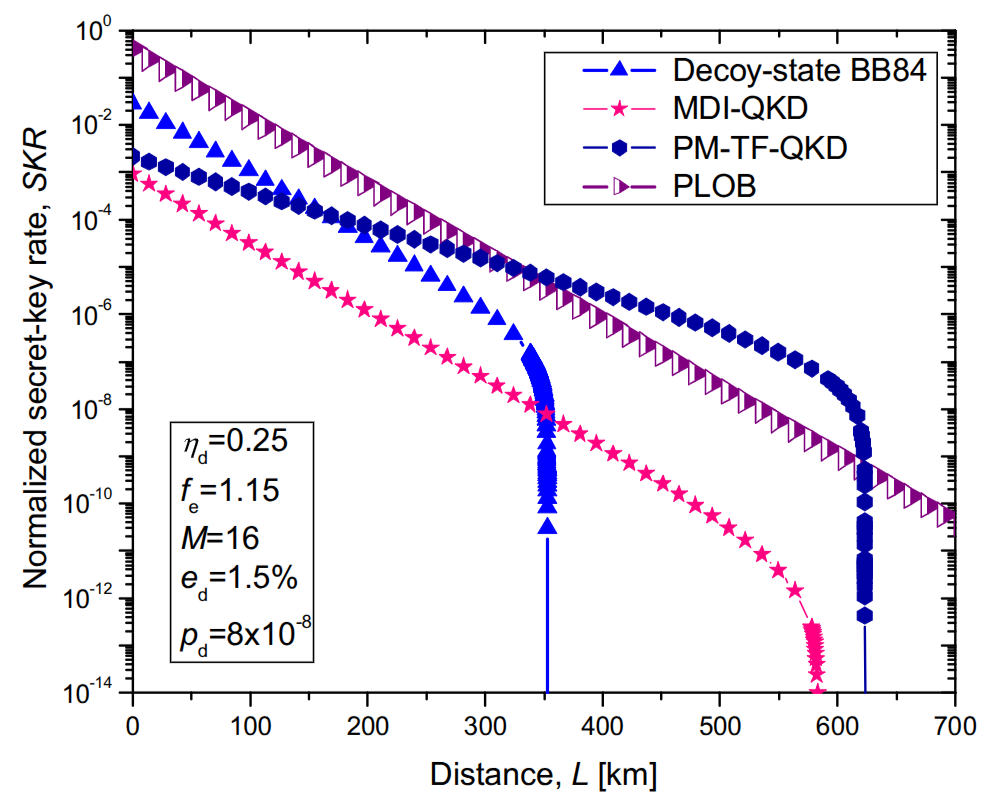
\includegraphics[width=0.5\textwidth]{chapters/figs/fig-6-21}
	\caption{پروتکل توزیع کلید کوانتومی (\lr{QKD}) میدان-دوقلوی آماده‌سازی-و-اندازه‌گیری در مقابل پروتکل‌های \lr{MDI-QKD} و \lr{BB84} حالت فریب در نمودار نرخ کلید مخفی نرمالیزه‌شده برحسب مسافت ارسال.}
	\label{fig:6-21}
\end{figure}

\section{مصالحه اطلاعات و تقویت حریم خصوصی}
\label{sec:6-9}
همان‌طور که پیش‌تر بحث شد، کلید خام ناقص است و ما باید مصالحه اطلاعات و تقویت حریم خصوصی را انجام دهیم تا همبستگی بین دنباله‌های آلیس و باب را افزایش داده و در عین حال، اطلاعات متقابل شنودگر (ایو) درباره نتیجه را تا سطح امنیت مطلوب کاهش دهیم.

\subsection{مصالحه اطلاعات}
\label{sec:6-9-1}
\lr{EA-QKD} شباهت‌های خاصی به پروتکل تولید (توافق) کلید مخفی نوع منبع دارد که در امنیت لایه فیزیکی مطرح است \cite{2}. در این مدل، آلیس، باب و ایو به پورت‌های خروجی متناظر $X$، $Y$ و $Z$ از منبعی که با تابع چگالی احتمال (\lr{PDF}) مشترک $f_{XYZ}$ مشخص می‌شود، دسترسی دارند. هر یک از آن‌ها تحقق‌های مستقل و با توزیع یکسان (\lr{i.i.d.}) از منبع را مشاهده می‌کنند که به‌ترتیب با $X^n$، $Y^n$ و $Z^n$ نشان داده می‌شوند. با توجه به اینکه تحقق‌های آلیس و باب کاملاً همبسته نیستند، آن‌ها باید خطاهای ناشی از اختلافات را اصلاح کنند. این مرحله در تولید کلید مخفی و \lr{QKD} معمولاً به عنوان مصالحه اطلاعات (یا صرفاً مصالحه) شناخته می‌شود. فرآیند مصالحه را می‌توان به عنوان مورد خاصی از کدگذاری منبع با اطلاعات جانبی\LTRfootnote{Source coding with side information} در نظر گرفت \cite{11, 106}. برای کدگذاری منبع $X$، از قضیه کدگذاری منبع شانون\LTRfootnote{Shannon's source coding theorem} می‌دانیم که نرخ $R_x$ باید تا حد امکان کوچک باشد اما نباید از آنتروپی منبع کمتر باشد؛ به عبارت دیگر $R_x > H(X)$. برای کدگذاری مشترک منبع ($XY, f_{XY}$) به نرخ $R > H(X,Y)$ نیاز داریم. اگر منابع را به‌طور مجزا کدگذاری کنیم، نرخ مورد نیاز $R > H(X) + H(Y)$ خواهد بود. با این حال، اسلپیان و ولف\LTRfootnote{Slepian and Wolf} در مرجع \cite{106} نشان داده‌اند که نرخ $R = H(X,Y)$ حتی برای کدگذاری مجزای منابع همبسته نیز کافی است. این ادعا معمولاً به عنوان قضیه اسلپیان-ولف شناخته می‌شود و می‌تواند به‌صورت زیر فرمول‌بندی شود \cite{11, 106}: ناحیه نرخ دستیابی‌پذیر\LTRfootnote{Achievable rate region} $\mathcal{R}$ (که برای آن احتمال خطا به صفر میل می‌کند) برای کدگذاری مجزای منبع همبسته ($XY, f_{XY}$) توسط رابطه زیر داده می‌شود:
\begin{equation}
	\mathcal{R} = \left\{ (R_x, R_y) : R_x \geq H(X|Y), R_y \geq H(Y|X), R_x + R_y \geq H(X,Y) \right\}
	\label{eq:6-56}
\end{equation}
شکل معمول ناحیه اسلپیان-ولف در شکل \ref{fig:6-22} ارائه شده است. اکنون اگر فرض کنیم که $(X, f_X)$ باید در حالی که $(Y, f_Y)$ به عنوان اطلاعات جانبی در دسترس است فشرده شود، آنگاه $H(X|Y)$ برای توصیف $X$ کافی است.







\begin{figure}[ht]
	\centering
	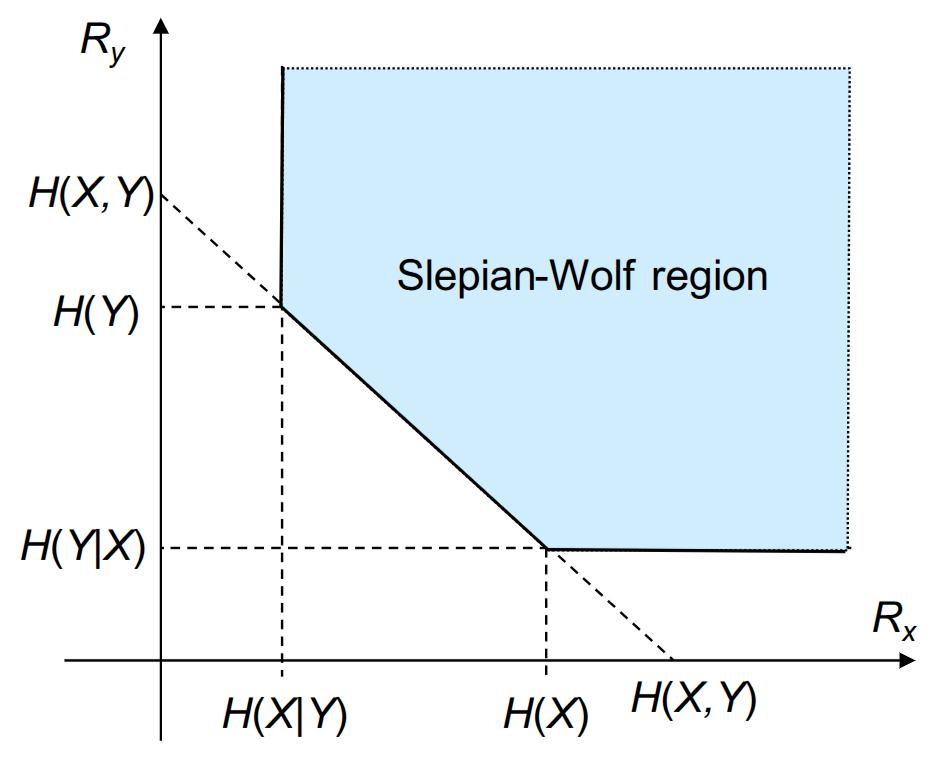
\includegraphics[width=0.5\textwidth]{chapters/figs/fig-6-22}
	\caption{ناحیه نرخ دستیابی‌پذیر معمول اسلپیان-ولف برای یک منبع همبسته ($XY, f_{XY}$).}
	\label{fig:6-22}
\end{figure}

با بازگشت به مسئله مصالحه خود، آلیس مشاهدات خود $X^n$ را فشرده می‌کند و باب آن‌ها را با کمک اطلاعات جانبی همبسته $Y^n$ رمزگشایی می‌نماید که در شکل \ref{fig:6-23} نشان داده شده است. رمزگذار منبع را می‌توان از کد کانال دستیابی‌پذیر به ظرفیت استخراج کرد. برای یک کد بررسی توازن کم‌چگال (\lr{LDPC})\LTRfootnote{Low-density parity-check (LDPC)} با مشخصات $(n,k)$، می‌توان از یک ماتریس بررسی توازن $\bm{H}$ با ابعاد $(n-k) \times n$ برای تولید سندرم\LTRfootnote{Syndrome} به‌صورت $\bm{s} = \bm{H}\bm{x}$ استفاده کرد که در آن $\bm{x}$ بردار مشاهده منبع گسسته بدون حافظه\LTRfootnote{Discrete Memoryless Source (DMS)} آلیس به طول $n$ است. از آنجا که $\bm{x}$ یک کلمه کد\LTRfootnote{Codeword} نیست، بردار سندرم با بردار تمام‌صفر متفاوت خواهد بود. بردار سندرم دارای طول $n-k$ است و می‌توان آن را به‌صورت $\bm{s} = [s_1, s_2, \dots, s_{n-k}]^T$ نمایش داد. به‌وضوح، بردار سندرم از طریق کانال عمومی احرازهویت‌شده (بدون خطا) به سمت باب ارسال می‌شود.

\begin{figure}[ht]
	\centering
	 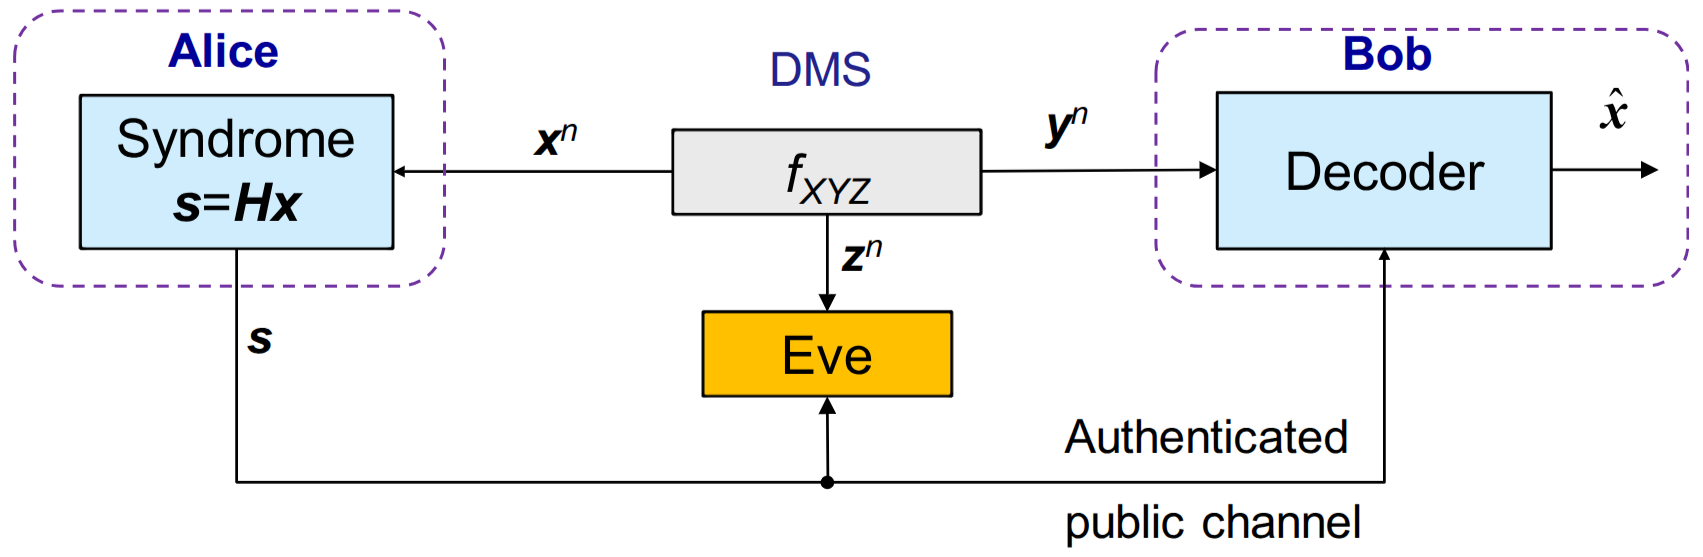
\includegraphics[width=0.8\textwidth]{chapters/figs/fig-6-23}
	\caption{مسئله مصالحه که به‌صورت کدگذاری منبع با اطلاعات جانبی مبتنی بر سندرم نمایش داده شده است.}
	\label{fig:6-23}
\end{figure}

هنگامی که باب بردار سندرم $\bm{s}$ را دریافت می‌کند، رمزگشای او سعی می‌کند بردار $\bm{x}$ را بر اساس $\bm{s}$ و بردار مشاهده باب $\bm{y}$ تعیین کند، به‌طوری که احتمال پسین\LTRfootnote{Posterior probability} را بیشینه نماید:
\begin{equation}
	\hat{\bm{x}} = \max P(\bm{y}|\bm{x}, \bm{s})
	\label{eq:6-57}
\end{equation}
و به‌وضوح، مسئله رمزگشایی مشابه رمزگشایی با بیشینه احتمال پسین (\lr{MAP})\LTRfootnote{Maximum a posteriori probability (MAP)} است. نرخ فشرده‌سازی برابر با $(n-k)/n = 1 - k/n$ است، در حالی که نرخ کد خطی $k/n$ می‌باشد. تعداد بیت‌های سندرم مورد نیاز برابر است با:
\begin{equation}
	n - k \geq nH(X^n|Y^n) = nH(X|Y)
	\label{eq:6-58}
\end{equation}
در عمل، الگوریتم‌های مصالحه کاربردی، یک مقدار بالاسری\LTRfootnote{Overhead} $OH > 0$ معرفی می‌کنند، به‌طوری که تعداد بیت‌های ارسال شده در کانال عمومی برابر با $nH(X|Y)(1 + OH)$ است. در پایان مرحله مصالحه، آلیس و باب دنباله مشترک $X^n$ با آنتروپی $nH(X)$ را با احتمال بالا به اشتراک می‌گذارند، بنابراین بازدهی مصالحه $\beta$ را می‌توان به‌صورت زیر نوشت:
\begin{equation}
	\beta = \frac{nH(X) - nH(X|Y)(1 + OH)}{nI(X; Y)} = 1 - OH \frac{H(X|Y)}{I(X; Y)} \leq 1
	\label{eq:6-59}
\end{equation}

پیچیدگی رمزگشایی \lr{MAP} در هنگام استفاده از کدگذاری \lr{LDPC} به‌طور بازدارنده‌ای بالا است؛ در عوض باید از الگوریتم مجموع-حاصل‌ضرب (\lr{SPA})\LTRfootnote{Sum-product algorithm (SPA)} با پیچیدگی کم (که با نام الگوریتم انتشار باور\LTRfootnote{Belief-propagation algorithm} نیز شناخته می‌شود) مطابق آنچه در مرجع \cite{107} توصیف شده است، استفاده کرد. با توجه به اینکه مشاهده آلیس $\bm{x}$ یک کلمه کد نیست، بیت‌های سندرم غیرصفر هستند. برای در نظر گرفتن این مسئله، هنگامی که بیت سندرم متناظر $s_c$ برابر با $1$ است، باید علامت نسبت لگاریتمی درست‌نمایی (\lr{LLR})\LTRfootnote{Log-likelihood ratio (LLR)} ارسالی از گره بررسی\LTRfootnote{Check node} $c$-ام به گره متغیر\LTRfootnote{Variable node} $v$-ام را تغییر دهیم. بر اساس مرجع \cite{108}، می‌توانیم \lr{SPA} در حوزه لگاریتم را به‌صورت زیر خلاصه کنیم. برای بهبود وضوح ارائه، از شاخص $v = 1, \dots, n$ برای نشان دادن گره‌های متغیر و از شاخص $c = 1, \dots, n-k$ برای نشان دادن گره‌های بررسی استفاده می‌کنیم. علاوه بر این، از نمادگذاری‌های زیر استفاده می‌شود: (الف) $N(c)$ برای نشان دادن {مجموعه گره‌های $v$ متصل به گره $c$}، (ب) $N(c) \setminus \{v\}$ برای نشان دادن {مجموعه گره‌های $v$ متصل به گره $c$ به‌جز گره $v$}، (ج) $N(v)$ برای نشان دادن {مجموعه گره‌های $c$ متصل به گره $v$}، و (د) $N(v) \setminus \{c\}$ برای نشان دادن {مجموعه گره‌های $c$ متصل به گره $v$ به‌جز گره $c$}.

فرمول‌بندی \lr{SPA} در حوزه لگاریتم برای کدگذاری منبع با اطلاعات جانبی به‌صورت زیر ارائه می‌شود:

\begin{enumerate}
	\item \textbf{مقداردهی اولیه:} برای گره‌های متغیر $v = 1, 2, \dots, n$؛ پیام‌های بیرونی\LTRfootnote{Extrinsic messages} $L_{vc}$ ارسالی از گره متغیر (\lr{v-node}) $v$ به گره بررسی (\lr{c-node}) $c$ را با نسبت‌های لگاریتمی درست‌نمایی کانال که با $L_{ch}(v)$ نشان داده می‌شوند، مقداردهی اولیه کنید؛ یعنی $L_{vc} = L_{ch}(v)$.
	\item \textbf{قانون به‌روزرسانی گره بررسی (گره $c$):} برای گره‌های بررسی $c = 1, 2, \dots, n-k$؛ مقدار $L_{cv} = (1 - 2s_c) \sum_{N(c) \setminus \{v\}} L_{v'c}$ را محاسبه کنید. عملگر باکس-پلاس\LTRfootnote{Box-plus operator} به‌صورت زیر تعریف می‌شود:
	\begin{equation}
		L_1 + L_2 = \prod_{k=1}^2 \text{sign}(L_k) \cdot \phi \left( \sum_{k=1}^2 \phi(|L_k|) \right)
		\label{eq:6-60}
	\end{equation}
	که در آن $\phi(x) = -\log \tanh(x/2)$ است. عملگر باکس برای مولفه‌های $|N(c) \setminus \{v\}|$ با اعمال بازگشتی نسخه دو-مولفه‌ای تعریف شده در بالا به‌دست می‌آید.
	\item \textbf{قانون به‌روزرسانی گره متغیر (گره $v$):} برای $v = 1, 2, \dots, n$؛ مقدار $L_{vc} = L_{ch}(v) + \sum_{N(v) \setminus \{c\}} L_{c'v}$ را برای تمام گره‌های $c$ که عنصر سطر $c$-ام و ستون $v$-ام ماتریس بررسی توازن $\bm{H}$ آن‌ها یک است (یعنی $h_{cv} = 1$)، تنظیم کنید.
	\item \textbf{تصمیم‌گیری بیت‌ها:} مقدار $L(v)$ را برای $v = 1, \dots, n$ با رابطه $L(v) = L_{ch}(v) + \sum_{N(v)} L_{c'v}$ به‌روزرسانی کرده و تصمیم‌گیری‌ها را به‌صورت زیر انجام دهید:
	$\hat{x}_v = 1$ اگر $L(v) < 0$ (در غیر این صورت $\hat{x}_v = 0$).
\end{enumerate}

بنابراین تنها تفاوت نسبت به \lr{SPA} متعارف در حوزه لگاریتم، معرفی ضریب ضرب $(1 - 2s_c)$ در قانون به‌روزرسانی گره $c$ است. علاوه بر این، درست‌نمایی‌های کانال $L_{ch}(v)$ باید از توزیع مشترک $f_{XY}$ به‌صورت $L_{ch}(v) = \log [f_{XY}(x_v = 0|y_v) / f_{XY}(x_v = 1|y_v)]$ محاسبه شوند. از آنجا که قانون به‌روزرسانی گره $c$ شامل توابع $\log$ و $\tanh$ است، می‌تواند از نظر محاسباتی سنگین باشد و برای کاهش پیچیدگی، باید از تقریب‌های با پیچیدگی کاهش‌یافته استفاده کرد.


تحلیل تقویت حریم خصوصی بر پایه آنتروپی شانون نیست، بلکه بر اساس آنتروپی رنی\LTRfootnote{Rényi entropy} انجام می‌شود \cite{114, 115, 116}. برای متغیر تصادفی گسسته $\bm{X}$ که مقادیری را از فضای نمونه\LTRfootnote{Sample space} $\{x_1, \dots, x_n\}$ می‌گیرد و طبق توزیع $P_{\bm{X}} = \{p_1, \dots, p_n\}$ توزیع شده است، آنتروپی رنی از مرتبه $\alpha$ برای $\bm{X}$ طبق مرجع \cite{115} به‌صورت زیر تعریف می‌شود:
\begin{equation}
	R_\alpha(\bm{X}) = \frac{1}{1-\alpha} \log_2 \left( \sum_{x \in \mathcal{X}} [P_{\bm{X}}(x)]^\alpha \right)
	\label{eq:6-60}
\end{equation}

آنتروپی رنی از مرتبه دو با نام آنتروپی برخورد\LTRfootnote{Collision entropy} نیز شناخته می‌شود. از نامساوی ینسن\LTRfootnote{Jensen's inequality} \cite{11} نتیجه می‌گیریم که آنتروپی برخورد توسط آنتروپی شانون محدود می‌شود، یعنی $R_2(\bm{X}) \leq H(\bm{X})$. در حالتی که $\alpha \to \infty$، آنتروپی رنی به کمینه-آنتروپی\LTRfootnote{Min-entropy} تبدیل می‌شود:
\begin{equation}
	\lim_{\alpha \to \infty} R_\alpha(\bm{X}) = -\log_2 \max_{x \in \mathcal{X}} P_{\bm{X}}(x) = H_\infty(\bm{X})
	\label{eq:6-61}
\end{equation}
در نهایت، با اعمال قاعده هوپیتال\LTRfootnote{l'Hôpital's rule} در حالت $\alpha \to 1$، آنتروپی رنی به همان آنتروپی شانون تبدیل می‌گردد:
\begin{equation}
	\lim_{\alpha \to 1} R_\alpha(\bm{X}) = -\sum_x P_{\bm{X}}(x) \log_2 P_{\bm{X}}(x) = H(\bm{X})
	\label{eq:6-62}
\end{equation}
ویژگی‌های آنتروپی رنی در مرجع \cite{115} خلاصه شده است. در رابطه با آنتروپی رنی شرطی، سه تعریف مختلف در مرجع \cite{116} به‌تفصیل مورد بحث قرار گرفته است که ما اولین مورد از آن‌ها را برمی‌گزینیم. فرض کنید توزیع مشترک برای $(\bm{X}, \bm{Y})$ با $P_{\bm{X,Y}}$ و توزیع برای $\bm{X}$ با $P_{\bm{X}}$ نشان داده شود. علاوه بر این، فرض کنید آنتروپی رنی متغیرهای تصادفی شرطی $\bm{X}|\bm{Y}=y$ که طبق $P_{\bm{X}|\bm{Y}=y}$ توزیع شده‌اند، با $R_\alpha(\bm{X}|\bm{Y}=y)$ نشان داده شود. آنگاه آنتروپی رنی شرطی را می‌توان به‌صورت زیر تعریف کرد:
\begin{equation}
	R_\alpha(\bm{X}|\bm{Y}) = \sum_y P_{\bm{Y}}(y) R_\alpha(\bm{X}|\bm{Y}=y) = \frac{1}{1-\alpha} \sum_y P_{\bm{Y}}(y) \log_2 \sum_x P_{\bm{X}|\bm{Y}}(x|y)^\alpha
	\label{eq:6-63}
\end{equation}
اطلاعات رنی متقابل\LTRfootnote{Mutual Rényi information} را نیز می‌توان به‌صورت زیر تعریف کرد:
\begin{equation}
	I_\alpha(\bm{X}; \bm{Y}) = R_\alpha(\bm{X}) - R_\alpha(\bm{X}|\bm{Y})
	\label{eq:6-64}
\end{equation}
که نسبت به $R_\alpha(\bm{Y}) - R_\alpha(\bm{Y}|\bm{X})$ متقارن نیست. علاوه بر این، همان‌طور که در مراجع \cite{115, 116} بحث شده است، این مقدار حتی می‌تواند منفی باشد.

بنت و همکاران در مرجع \cite{23} قضیه تقویت حریم خصوصی زیر را اثبات کرده‌اند (قضیه ۳ را ببینید): فرض کنید $\bm{X}$ یک متغیر تصادفی با توزیع $P_{\bm{X}}$ و آنتروپی رنی مرتبه دو $R_2(\bm{X})$ باشد. همچنین فرض کنید $\bm{G}$ متغیر تصادفی نشان‌دهنده انتخاب تصادفی و یکنواخت عضوی از توابع هش سراسری $\{0,1\}^n \to \{0,1\}^k$ باشد. در این صورت نامساوی‌های زیر برقرار هستند \cite{23}:
\begin{equation}
	H(\bm{G}(\bm{X})|\bm{G}) \leq R_2(\bm{G}(\bm{X})|\bm{G}) \leq k + \log_2 (1 + 2^{k-R_2(\bm{X})}) \leq k + \frac{2^{k-R_2(\bm{X})}}{\ln 2}
	\label{eq:6-65}
\end{equation}
بنت و همکاران همچنین نتیجه\LTRfootnote{Corollary} زیر را از قضیه تقویت حریم خصوصی اثبات کرده‌اند \cite{23} (همچنین ببینید \cite{110}): فرض کنید $\bm{S} \in \{0,1\}^n$ متغیر تصادفی نشان‌دهنده دنباله مشترک بین آلیس و باب باشد و $\bm{E}$ متغیر تصادفی نشان‌دهنده دانشی باشد که ایو توانسته درباره $\bm{S}$ به‌دست آورد، به‌طوری‌که یک تحقق خاص از $\bm{E}$ با $e$ نشان داده می‌شود. اگر معلوم باشد که آنتروپی رنی شرطی مرتبه دو $R_2(\bm{S}|\bm{E}=e)$ حداقل برابر با $r_2$ است و آلیس و باب کلید مخفی را به‌صورت $\bm{K} = \bm{G}(\bm{S})$ انتخاب کنند (که در آن $\bm{G}$ یک تابع هش است که به‌طور تصادفی و یکنواخت از خانواده توابع هش جهانی-$2$ در $\{0,1\}^n \to \{0,1\}^k$ انتخاب شده است)، آنگاه رابطه زیر معتبر است:
\begin{equation}
	H(\bm{K}|\bm{G}, \bm{E}=e) \geq k - \frac{2^{k-r_2}}{\ln 2}
	\label{eq:6-66}
\end{equation}

کاچین\LTRfootnote{Cachin} در مرجع \cite{117} لم آنتروپی رنی زیر را اثبات کرده است (همچنین ببینید \cite{118}): فرض کنید $\bm{X}$ و $\bm{Q}$ دو متغیر تصادفی باشند و $s > 0$. آنگاه با احتمالی حداقل برابر با $1 - 2^{-s}$، رابطه زیر برقرار است \cite{117, 118}:
\begin{equation}
	R_2(\bm{X}) \geq R_2(\bm{X}|\bm{Q}=q) - \log |\bm{Q}| - 2s - 2
	\label{eq:6-67}
\end{equation}
اطلاعات کل در دسترس ایو متشکل از مشاهدات او $\bm{Z}^n$ از منبع تصادفی مشترک و بیت‌های اضافی مبادله شده در مرحله مصالحه اطلاعات روی کانال عمومی احرازهویت‌شده است که با متغیر تصادفی $\bm{Q}$ نشان داده می‌شود. بر اساس لم کاچین، می‌توانیم بنویسیم:
\begin{equation}
	R_2(\bm{S}|\bm{Z}^n=z_n) \geq R_2(\bm{S}|\bm{Z}^n=z_n, \bm{Q}=q) - \log |\bm{Q}| - 2s - 2 \text{ با احتمال } 1 - 2^{-s}
	\label{eq:6-68}
\end{equation}
می‌دانیم که $R_2(\bm{X}) \leq H(\bm{X})$، بنابراین نتیجه می‌گیریم که $R_2(\bm{S}|\bm{Z}^n=z_n) \leq H(\bm{S}|\bm{Z}^n=z_n)$ و از این رو، می‌توانیم $R_2(\bm{S}|\bm{Z}^n=z_n)$ را به‌صورت زیر از بالا محدود کنیم:
\begin{equation}
	R_2(\bm{S}|\bm{Z}^n=z_n) \leq nH(X|Z)
	\label{eq:6-69}
\end{equation}
بر اساس رابطه \eqref{eq:6-68}، می‌توانیم $R_2(\bm{S}|\bm{Z}^n=z_n, \bm{Q}=q)$ را به‌صورت زیر از پایین محدود کنیم:
\begin{equation}
	R_2(\bm{S}|\bm{Z}^n=z_n, \bm{Q}=q) \geq nH(X|Z) - \log |\bm{Q}| - 2s - 2 \text{ با احتمال } 1 - 2^{-s}
	\label{eq:6-70}
\end{equation}
از آنجا که تعداد بیت‌های مبادله شده در کانال عمومی، $\log |\bm{Q}|$، تقریباً برابر با $nH(X|Y)(1 + OH)$ است، برای $n$ به اندازه کافی بزرگ، نامساوی قبلی به‌صورت زیر در می‌آید:
\begin{equation}
	\underbrace{nH(X|Z) - nH(X|Y)(1 + OH) - 2s - 2}_{r_2} \geq R_2(\bm{S}|\bm{Z}^n=z_n, \bm{Q}=q) \text{ با احتمال } 1 - 2^{-s}
	\label{eq:6-71}
\end{equation}
از رابطه \eqref{eq:6-66} نتیجه می‌گیریم که $k - r_2 = -k_2 < 0$ است، که تضمین می‌کند برای $k_2 > 0$، عدم قطعیت ایو درباره کلید با احتمالی حداقل برابر با $1 - 2^{-s}$ به‌صورت زیر از پایین محدود می‌شود:
\begin{equation}
	H(\bm{K}|\bm{E}) \geq k - \frac{2^{-k_2}}{\ln 2}
	\label{eq:6-72}
\end{equation}


\section{توزیع کلید کوانتومی با متغیر پیوسته}
\label{sec:6-10}
خوانندگانی که با اپتیک کوانتومی آشنا نیستند، باید ابتدا بخش‌های \ref{sec:5-4} و \ref{sec:5-8} در فصل \ref{chap:5} را مطالعه کنند. \lr{CV-QKD} را می‌توان یا با استفاده از آشکارسازی هموداین\LTRfootnote{Homodyne detection} پیاده‌سازی کرد که در آن در هر لحظه تنها یک مؤلفه مربعی\LTRfootnote{Quadrature component} اندازه‌گیری می‌شود (به دلیل اصل عدم قطعیت)، همان‌طور که در شکل \ref{fig:6-24} نشان داده شده است؛ و یا با استفاده از آشکارسازی هتروداین\LTRfootnote{Heterodyne detection (HD)} (\lr{HD}) که در آن از یک \lr{BS} و دو فتودتکتور متعادل\LTRfootnote{Balanced photodetectors} برای اندازه‌گیری هم‌زمان هر دو مؤلفه مربعی استفاده می‌شود، مطابق آنچه در شکل \ref{fig:6-25} تصویر شده است. \lr{HD} می‌تواند اطلاعات متقابل بین آلیس و باب را در مقایسه با طرح آشکارسازی هموداین دوبرابر کند، که البته این امر به قیمت تلفات اضافی $3$ \lr{dB} ناشی از \lr{BS} تمام می‌شود. برای کاهش نویز فاز، سیگنال‌های کوانتومی معمولاً همراه با یک تُن پایلوت\LTRfootnote{Pilot-tone} پرتوانِ تسهیم‌شده در حوزه زمان ارسال می‌شوند تا پایه‌های اندازه‌گیری آلیس و باب با یکدیگر هم‌راستا شوند. با قضاوت از روی تعداد فزاینده مقالات مرتبط با \lr{CV-QKD} \cite{8, 119, 120, 121, 122, 123, 124, 125, 126, 127, 128, 129, 130, 131, 132, 133, 134, 135, 136, 137, 138, 139, 140, 141, 142, 143, 144, 145}، پژوهش‌ها در این حوزه به دلیل سازگاری آن‌ها با فناوری‌های پیشرفته مخابرات نوری در حال شتاب گرفتن است. سیستم \lr{CV-QKD} هنگام استفاده از مصالحه مستقیم\LTRfootnote{Direct reconciliation}، با محدودیت تلفات $3$ \lr{dB} در گذردهی مواجه می‌شود. برای جلوگیری از این مشکل، از روش‌های مصالحه معکوس\LTRfootnote{Reverse reconciliation} \cite{146} یا پس‌گزینش\LTRfootnote{Postselection} \cite{127} استفاده می‌شود. استراتژی‌های مختلف شنود که پیش‌تر بحث شد، برای سیستم‌های \lr{CV-QKD} نیز قابل اعمال هستند. نشان داده شده است که برای مدولاسیون گاوسی، حمله گاوسی بهینه ترین حمله برای هر دو نوع حملات انفرادی \cite{133} و حملات دسته‌جمعی \cite{134, 135} است. در این بخش از فصل، تمرکز خود را بر \lr{CV-QKD} با مدولاسیون گاوسی معطوف می‌کنیم. برای پیاده‌سازی \lr{CV-QKD}، هم می‌توان از حالت‌های فشرده\LTRfootnote{Squeezed states} و هم از حالت‌های همدوس استفاده کرد.

\begin{figure}[ht]
	\centering
	 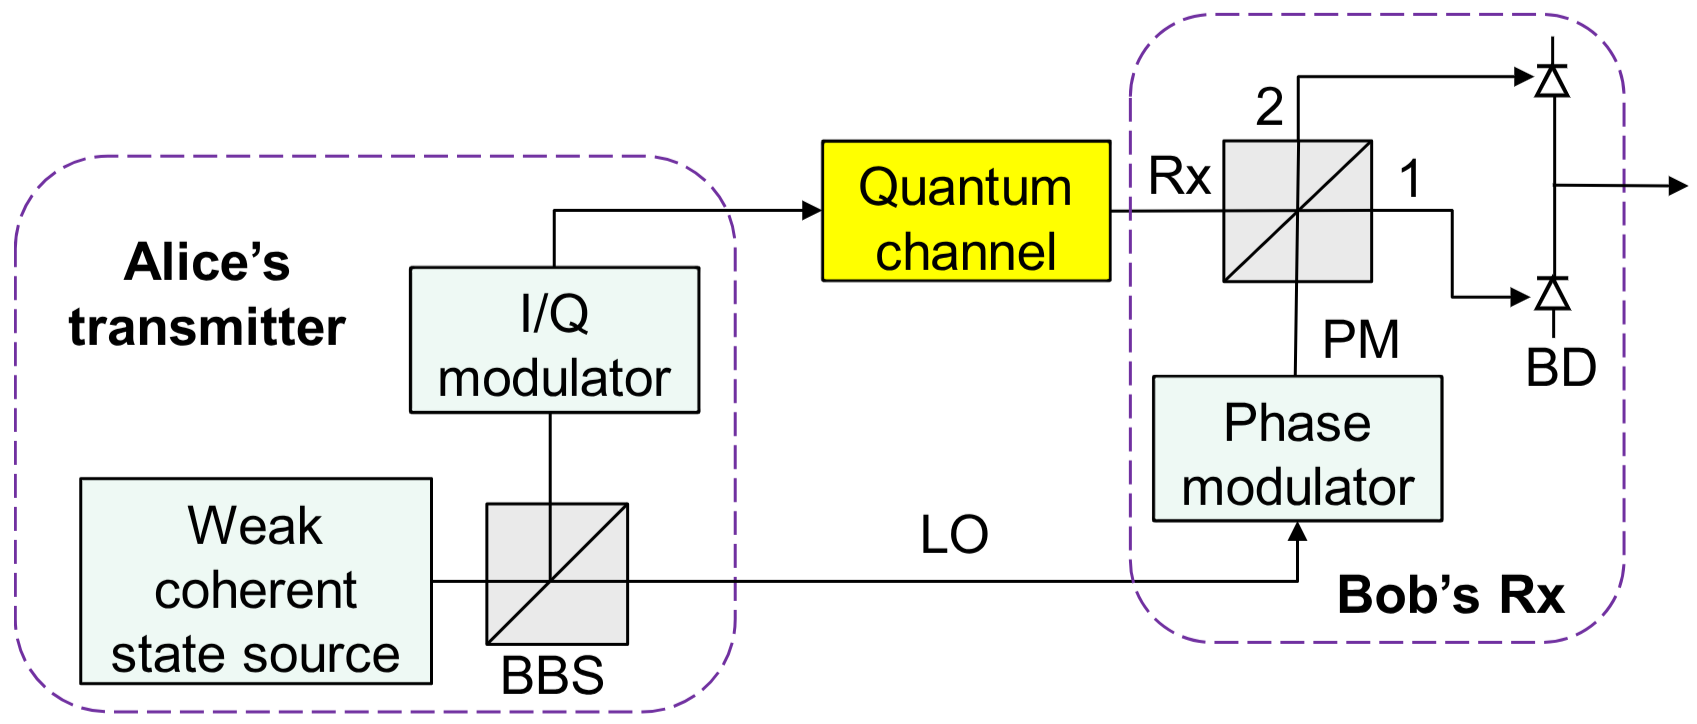
\includegraphics[width=0.8\textwidth]{chapters/figs/fig-6-24}
	\caption{پروتکل‌های توزیع کلید کوانتومی با متغیر پیوسته مبتنی بر مدولاسیون گاوسی با آشکارسازی هموداین. \lr{BBS}: تقسیم‌کننده پرتو متعادل؛ \lr{BD}: آشکارساز متعادل.}
	\label{fig:6-24}
\end{figure}

\begin{figure}[ht]
	\centering
	 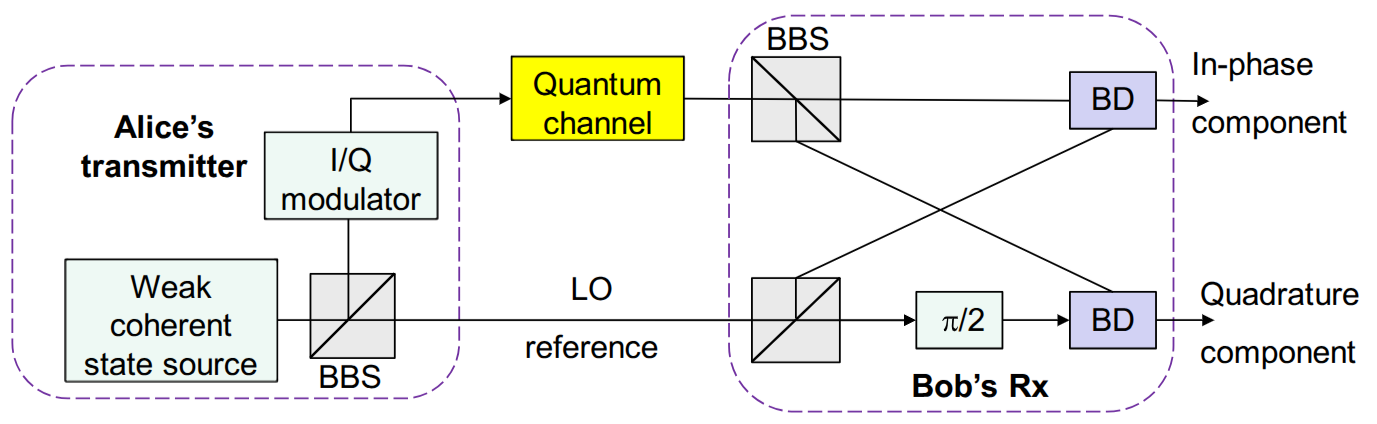
\includegraphics[width=0.8\textwidth]{chapters/figs/fig-6-25}
	\caption{پروتکل‌های توزیع کلید کوانتومی با متغیر پیوسته مبتنی بر مدولاسیون گاوسی با آشکارسازی هتروداین. \lr{BBS}: تقسیم‌کننده پرتو متعادل؛ \lr{BD}: آشکارساز متعادل (نشان داده شده در شکل \ref{fig:6-24}).}
	\label{fig:6-25}
\end{figure}



\subsection{طرح‌های آشکارسازی هموداین و هتروداین}
\label{subsec:6-10-1}
در طرح آشکارسازی هموداین\LTRfootnote{Homodyne detection} که در شکل \ref{fig:6-24} ارائه شده و رایج‌ترین نوع اندازه‌گیری در سیستم‌های متغیر پیوسته (\lr{CV}) محسوم می‌شود، ما یکی از دو مؤلفه مربعی را اندازه‌گیری می‌کنیم؛ زیرا طبق اصل عدم قطعیت، نمی‌توانیم هر دو مؤلفه مربعی را به‌طور هم‌زمان اندازه‌گیری کنیم. عملگرهای اندازه‌گیری، تصویرگرهایی روی پایه مؤلفه مربعی $|I\rangle\langle I|$ یا $|Q\rangle\langle Q|$ هستند و نتایج متناظر دارای تابع چگالی احتمال (\lr{PDF}) $f(I)$ یا $f(Q)$ می‌باشند که از طریق انتگرال‌گیری حاشیه‌ای\LTRfootnote{Marginal integration} از تابع ویگنر\LTRfootnote{Wigner function} (معرفی شده در رابطه $5.144$) به‌دست می‌آیند، که برای تک‌مُد به‌صورت زیر در می‌آید:
\begin{equation*}
	f(I) = \int W(I, Q) dQ; \quad f(Q) = \int W(I, Q) dI
\end{equation*}
زمانی که بیش از یک مُد بوزونی\LTRfootnote{Bosonic modes} در باریکه نوری وجود داشته باشد، باید هموداین کردن جزئی\LTRfootnote{Partial homodyning} را اعمال کرده و همچنین روی هر دو مؤلفه مربعی تمام مدهای دیگر انتگرال‌گیری انجام دهیم.

در \lr{CV-QKD} مبتنی بر مدولاسیون گاوسی با آشکارسازی هموداین \cite{2, 8} که در شکل \ref{fig:6-24} نشان داده شده است، در هر لحظه تنها یک مؤلفه مربعی اندازه‌گیری می‌شود. این پروتکل معمولاً با نام پروتکل \lr{CV-QKD} \lr{GG02} شناخته می‌شود که به نام نویسندگان آن، گروس‌هانز\LTRfootnote{Grosshans} و گرنژیه\LTRfootnote{Grangier} که آن را در سال $2002$ پیشنهاد کردند، نام‌گذاری شده است \cite{146}. آلیس باریکه لیزر را که به‌عنوان یک منبع \lr{WCS} عمل می‌کند، به‌قدر کافی تضعیف کرده و از تقسیم‌کننده پرتو متعادل (\lr{BBS})\LTRfootnote{Balanced beam splitter (BBS)} برای تقسیم سیگنال به دو بخش استفاده می‌کند. خروجی بالایی \lr{BBS} به‌عنوان ورودی به مدولاتور \lr{I/Q} استفاده می‌شود تا حالت گاوسی را در مکان مورد نظر در صفحه \lr{I-Q} قرار دهد و $|\alpha\rangle = |I + jQ\rangle$ را به‌دست آورد و همچنین واریانس آلیس را کنترل کند. خروجی دوم \lr{BBS} برای ارسال سیگنال مرجع نوسان‌ساز محلی (\lr{LO})\LTRfootnote{Local oscillator (LO)} برای باب استفاده می‌شود. از آنجا که عملکرد تقسیم‌کننده پرتو با ماتریس $B_{BS} = \frac{1}{\sqrt{2}} \begin{bmatrix} 1 & 1 \\ 1 & -1 \end{bmatrix}$ توصیف می‌شود، عملگرهای نابودی\LTRfootnote{Annihilation operators} در خروجی \lr{BBS} باب به‌صورت زیر خواهند بود:
\begin{equation}
	\begin{bmatrix} a_1 \\ a_2 \end{bmatrix} = \frac{1}{\sqrt{2}} \begin{bmatrix} 1 & 1 \\ 1 & -1 \end{bmatrix} \begin{bmatrix} a_{Rx} \\ a_{PM} \end{bmatrix} = \frac{1}{\sqrt{2}} \begin{bmatrix} a_{Rx} + a_{PM} \\ a_{Rx} - a_{PM} \end{bmatrix}
	\label{eq:6-73}
\end{equation}
که در آن عملگرهای تولید (نابودی) در ورودی‌های \lr{BBS} گیرنده ($Rx$ و $PM$) به‌ترتیب با $a_{Rx}^\dagger (a_{Rx})$ و $a_{PM}^\dagger (a_{PM})$ نشان داده شده‌اند. عملگرهای تعداد\LTRfootnote{Number operators} در خروجی‌های یک و دو \lr{BBS} گیرنده اکنون می‌توانند به‌صورت زیر بیان شوند:
\begin{equation}
	\hat{n}_1 = a_1^\dagger a_1 = \frac{1}{2} (a_{PM}^\dagger + a_{Rx}^\dagger)(a_{PM} + a_{Rx}); \quad \hat{n}_2 = a_2^\dagger a_2 = \frac{1}{2} (a_{PM}^\dagger - a_{Rx}^\dagger)(a_{PM} - a_{Rx})
	\label{eq:6-74}
\end{equation}
خروجی یک آشکارساز متعادل (\lr{BD})\LTRfootnote{Balanced detector (BD)} با فرض پاسخ‌دهی فتودیود $R_{ph} = 1 A/W$، (برحسب واحد نویز شات\LTRfootnote{Shot-noise unit} یا \lr{SNU}) به‌صورت زیر داده می‌شود:
\begin{equation}
	\hat{i}_{BD} = 4(\hat{n}_1 - \hat{n}_2) = 4(a_{PM}^\dagger a_{Rx} + a_{Rx}^\dagger a_{PM})
	\label{eq:6-75}
\end{equation}
خروجی مدولاسیون فاز را می‌توان برحسب \lr{SNU} به‌صورت $a_{PM} = |\alpha| e^{j\theta} / \sqrt{2}$ نمایش داد و پس از جایگذاری در \eqref{eq:6-75} به‌دست می‌آوریم:
\begin{equation}
	\hat{i}_{BD} = 4 \left( \frac{|\alpha| e^{-j\theta}}{\sqrt{2}} a_{Rx} + a_{Rx}^\dagger \frac{|\alpha| e^{j\theta}}{\sqrt{2}} \right) = 2\sqrt{2} |\alpha| (e^{-j\theta} a_{Rx} + e^{j\theta} a_{Rx}^\dagger)
	\label{eq:6-76}
\end{equation}
در غیاب ایو، منظومه سیگنال دریافتی $a_{Rx} = (\bm{I} + j\bm{Q})/2$ خواهد بود که پس از جایگذاری در معادله قبلی، به‌دست می‌آوریم:
\begin{equation}
	\begin{aligned}
		\hat{i}_{BD} &= |\alpha| [ (\cos \theta, \sin \theta) \ones \cdot (I \hat{I}, -Q \hat{Q}) + (\cos \theta, \sin \theta) \ones \cdot (I \hat{I}, Q \hat{Q}) ] \\
		&= |\alpha| (\cos \theta \cdot I \hat{I} + \sin \theta \cdot Q \hat{Q}).
		\label{eq:6-77}
	\end{aligned}
\end{equation}
باب مؤلفه هم‌فاز را با انتخاب $\theta = 0$ برای به‌دست آوردن $|\alpha|\bm{I}$ و مؤلفه مربعی را با تنظیم $\theta = \pi/2$ برای به‌دست آوردن $|\alpha|\bm{Q}$ اندازه‌گیری می‌کند.

نظریه آشکارسازی هتروداین\LTRfootnote{Heterodyne detection (HD)} نوری در مرجع \cite{147} توسعه یافته است. \lr{HD} متناظر با تصویر کردن بر روی حالت‌های همدوس است، یعنی $M(\alpha) \sim |\alpha\rangle\langle\alpha|$. این نظریه به \lr{POVM}\LTRfootnote{Positive operator-valued measure} مبتنی بر تصویر کردن روی حالت‌های گاوسی خالص تعمیم یافته است \cite{148, 149}. برای \lr{CV-QKD} با مدولاسیون گاوسی مبتنی بر \lr{HD}، سمت فرستنده مشابه نسخه آشکارسازی همدوس است. در گیرنده \lr{HD} نشان داده شده در شکل \ref{fig:6-25}، سیگنال کوانتومی با استفاده از \lr{BBS} تقسیم می‌شود؛ یک خروجی برای اندازه‌گیری مؤلفه هم‌فاز (شاخه بالایی) استفاده می‌شود، در حالی که خروجی دیگر (شاخه پایینی) به‌عنوان ورودی به \lr{BD} دوم برای آشکارسازی مؤلفه مربعی به کار می‌رود. سیگنال مرجع کلاسیک \lr{LO} نیز توسط \lr{BBS} تقسیم می‌شود، به‌طوری که خروجی بالایی به‌عنوان ورودی به \lr{BD} هم‌فاز استفاده شده و خروجی دیگر، پس از مدولاسیون فاز برای اعمال جابه‌جایی فاز $\pi/2$، به‌عنوان ورودی \lr{LO} به \lr{BD} مربعی جهت آشکارسازی مؤلفه مربعی به کار می‌رود. به این ترتیب هر دو مؤلفه مربعی می‌توانند به‌طور هم‌زمان اندازه‌گیری شوند و اطلاعات متقابل می‌تواند دوبرابر شود. از سوی دیگر، \lr{BBS} باعث تضعیف $3$ \lr{dB} سیگنال کوانتومی می‌شود.



\subsection{پروتکل‌های مبتنی بر حالت فشرده}
\label{sec:6-10-2}
پروتکل‌های مبتنی بر حالت فشرده\LTRfootnote{Squeezed state-based protocols} از اصل عدم قطعیت هایزنبرگ\LTRfootnote{Heisenberg uncertainty principle} بهره می‌گیرند که بیان می‌کند اندازه‌گیری هر دو مؤلفه مربعی با دقت کامل غیرممکن است. برای اعمال اطلاعات، آلیس به‌طور تصادفی انتخاب می‌کند که از درجه آزادی\LTRfootnote{Degree-of-freedom (DOF)} (\lr{DOF}) هم‌فاز یا مربعی استفاده کند، همان‌طور که در شکل \ref{fig:6-26-a} تصویر شده است. در قاعده کدگذاری آلیس $I$ (زمانی که از \lr{DOF} هم‌فاز استفاده می‌شود)، حالت فشرده بر روی مؤلفه هم‌فاز (با پارامتر فشردگی $s_I < 1$) به‌صورت زیر (در واحد \lr{SNU}) اعمال می‌شود:
\begin{equation}
	X_{A,I} \sim |x_{A,I}; s_I\rangle, \quad s_I < 1; \quad X_{A,I} \sim \mathcal{N}(0, \sqrt{v_{A,I}})
	\label{eq:6-78}
\end{equation}
دامنه از یک منبع گاوسی با میانگین صفر و واریانس $v_{A,I}$ انتخاب می‌شود. از سوی دیگر، در قاعده کدگذاری آلیس $Q$ (زمانی که از مؤلفه مربعی استفاده می‌شود)، حالت فشرده بر روی مؤلفه مربعی (با پارامتر فشردگی $s_Q > 1$) اعمال شده و می‌توانیم بنویسیم (در واحد \lr{SNU}):
\begin{equation}
	X_{A,Q} \sim |x_{A,Q}; s_Q\rangle, \quad s_Q > 1; \quad X_{A,Q} \sim \mathcal{N}(0, \sqrt{v_{A,Q}})
	\label{eq:6-79}
\end{equation}
واریانس‌های حالت‌های فشرده $I$ و $Q$ به‌ترتیب برابر با $V(\hat{I}) = s_I^2 = s_I$ و $V(\hat{Q}) = s_Q^2 = 1/s_Q$ خواهند بود (همان‌طور که در بالا شرح داده شد). در سمت گیرنده، باب به‌طور تصادفی انتخاب می‌کند که مؤلفه هم‌فاز یا مربعی را اندازه‌گیری کند. آلیس و باب قواعد کدگذاری به‌کار رفته توسط خود را برای اندازه‌گیری مؤلفه مربعی به ازای هر حالت فشرده مبادله می‌کنند و در فرآیند غربال‌گری، تنها مواردی را که در آن‌ها مؤلفه مربعی یکسانی را اندازه‌گیری کرده‌اند، نگه می‌دارند. بنابراین، این پروتکل بسیار شبیه به پروتکل \lr{BB84} است. پس از آن، مرحله مصالحه اطلاعات و متعاقب آن تقویت حریم خصوصی انجام می‌شود.

از دیدگاه ایو، حالت‌های مخلوط\LTRfootnote{Mixed states} متناظر زمانی که آلیس از \lr{DOF} هم‌فاز یا مربعی استفاده کرده است، به‌صورت زیر خواهد بود \cite{8}:
\begin{equation}
	\rho_I = \int f_{\mathcal{N}}(0, \sqrt{v_{A,I}}) |x; s_I\rangle \langle x; s_I| dx; \quad \rho_Q = \int f_{\mathcal{N}}(0, \sqrt{v_{A,Q}}) |x; s_Q\rangle \langle x; s_Q| dx
	\label{eq:6-80}
\end{equation}

\begin{figure}[ht]
	\centering
	\subfigure[\lr{CV-QKD} مبتنی بر حالت فشرده]{\label{fig:6-26-a}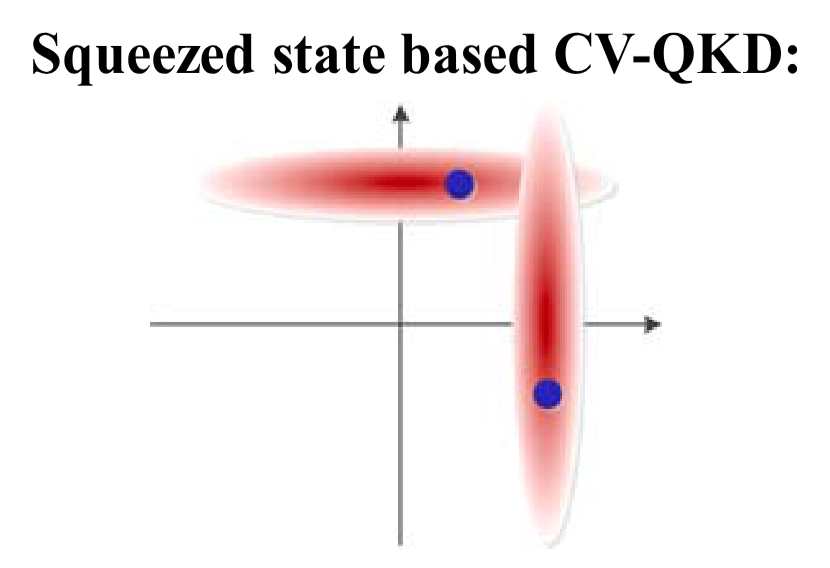
\includegraphics[width=0.42\textwidth]{chapters/figs/fig-6-26-a}}
	\hfill
	\subfigure[\lr{CV-QKD} مبتنی بر حالت همدوس]{\label{fig:6-26-b}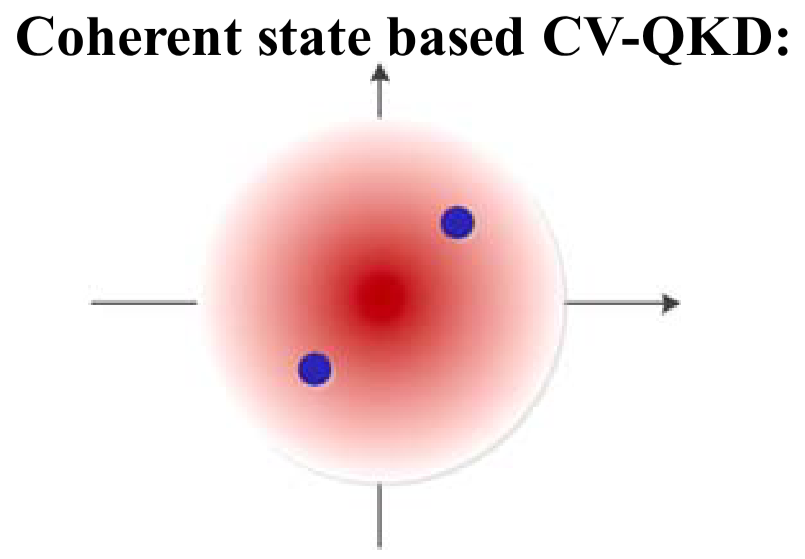
\includegraphics[width=0.42\textwidth]{chapters/figs/fig-6-26-b}}
	\caption{تصویرسازی اصول عملکرد پروتکل‌های مبتنی بر حالت فشرده (\subref{fig:6-26-a}) و همدوس (\subref{fig:6-26-b}).}
	\label{fig:6-26}
\end{figure}


که در آن $f_{\mathcal{N}}(0,s)$ توزیع گاوسی با میانگین صفر و واریانس $s^2$ است. هنگامی که شرط $\rho_I = \rho_Q$ برقرار باشد، ایو نمی‌تواند تشخیص دهد که آلیس اطلاعات را روی حالت فشرده $I$ یا $Q$ اعمال کرده است. با توجه به اینکه تولید حالت‌های فشرده بسیار دشوارتر از حالت‌های همدوس است، تمرکز خود را بر پروتکل‌های \lr{CV-QKD} مبتنی بر حالت همدوس معطوف می‌کنیم.

\subsection{پروتکل‌های توزیع کلید کوانتومی با متغیر پیوسته مبتنی بر حالت همدوس}
\label{subsec:6-10-3}
در پروتکل‌های مبتنی بر حالت همدوس، که اصول عملکرد آن‌ها در شکل \ref{fig:6-26} (\subref{fig:6-26-b}) ارائه شده است، تنها یک قاعده کدگذاری برای آلیس وجود دارد:
\begin{equation}
	X_{A,I}; X_{A,Q} \sim X_{A,I} + jX_{A,Q}; \quad X_{A,I} \sim \mathcal{N}(0, \sqrt{v_A}); \quad X_{A,Q} \sim \mathcal{N}(0, \sqrt{v_A})
	\label{eq:6-81}
\end{equation}
به عبارت دیگر، آلیس با کمک دستگاه ارائه شده در شکل \ref{fig:6-25}، به‌طور تصادفی نقطه‌ای را در فضای دوبعدی ($I,Q$) از یک توزیع گاوسی متقارن دایره‌ای با میانگین صفر انتخاب می‌کند. به‌وضوح، هر دو مؤلفه مربعی دارای عدم قطعیت یکسانی هستند. در اینجا نیز از اصل عدم قطعیت هایزنبرگ استفاده می‌کنیم که بیان می‌دارد اندازه‌گیری هر دو مؤلفه مربعی با دقت کامل غیرممکن است. برای گیرنده هموداین، باب اندازه‌گیری تصادفی را روی $\hat{I}$ یا $\hat{Q}$ انجام می‌دهد؛ فرض کنید نتیجه اندازه‌گیری او با $Y_B$ نشان داده شود. وقتی باب $\hat{I}$ را اندازه‌گیری می‌کند، اندازه‌گیری او ($Y_B$) با $X_{A,I}$ همبسته است. از سوی دیگر، وقتی باب $\hat{Q}$ را اندازه‌گیری می‌کند، نتیجه اندازه‌گیری او ($Y_B$) با $X_{A,Q}$ همبسته است. به‌وضوح، باب قادر است با استفاده از حالت همدوس گاوسی، یک مختصات واحد از نقطه منظومه سیگنال ارسال شده توسط آلیس را اندازه‌گیری کند. سپس باب اعلام می‌کند که در هر بازه سیگنال‌دهی کدام مؤلفه مربعی را اندازه‌گیری کرده است و آلیس مختصاتی را انتخاب می‌کند که با مؤلفه مربعی اندازه‌گیری شده توسط باب مطابقت دارد. باقی پروتکل مشابه پروتکل مبتنی بر حالت فشرده است.

از دیدگاه ایو، حالت مخلوط به‌صورت زیر خواهد بود:
\begin{equation}
	\rho = \int f_{\mathcal{N}}(0, \sqrt{v_A}) f_{\mathcal{N}}(0, \sqrt{v_A}) |I + jQ\rangle \langle I + jQ| dI dQ
	\label{eq:6-82}
\end{equation}
در اینجا $v_A$ واریانس مدولاسیون آلیس در واحد \lr{SNU} است. برای ارسال بدون تلفات، واریانس کل متغیر تصادفی باب در واحد \lr{SNU} به‌صورت زیر خواهد بود:
\begin{equation}
	V(Y_B) = \text{Var}(Y_B) = v_A + 1
	\label{eq:6-83}
\end{equation}
که از جمله مدولاسیون آلیس $v_A$ و واریانس نوسانات ذاتی حالت همدوس (که برابر با $1$ است) تشکیل شده است.

برای ارسال با تلفات\LTRfootnote{Lossy transmission}، کانال را می‌توان به‌صورت یک تقسیم‌کننده پرتو با تضعیف $0 \leq T \leq 1$ مدل‌سازی کرد، همان‌طور که در شکل \ref{fig:6-27} تصویر شده است. از این شکل نتیجه می‌گیریم که حالت خروجی $x_B$ را می‌توان برحسب حالت ورودی $x_A$ و حالت پایه\LTRfootnote{Ground state} $x_0$ به‌صورت زیر نشان داد:
\begin{equation}
	x_B = \sqrt{T} x_A + \sqrt{1-T} x_0 = \sqrt{T} (x_A + \sqrt{\chi_{\text{line}}} x_0); \quad \chi_{\text{line}} = (1-T)/T = 1/T - 1
	\label{eq:6-84}
\end{equation}
برای ارسال با تلفات، زمانی که به جای حالت‌های خلاء از مدولاسیون گاوسی حالت‌های همدوس استفاده می‌شود، رابطه قبلی باید به‌صورت زیر اصلاح گردد:
\begin{equation}
	x_B = \sqrt{T} (x_A + \sqrt{\chi_{\text{line}}} x_0); \quad \chi_{\text{line}} = (1-T)/T + \epsilon = 1/T - 1 + \epsilon; \quad \epsilon \geq 0
	\label{eq:6-85}
\end{equation}
که در آن $\epsilon$ نشان‌دهنده نویز اضافی\LTRfootnote{Excess noise} است.


\begin{figure}[ht]
	\centering
	% \includegraphics[width=0.8\textwidth]{fig6-27}
	\caption{تصویرسازی کانال ارسال با تلفات.}
	\label{fig:6-27}
\end{figure}

نخستین جمله در $\chi_{\text{line}}$ مربوط به تضعیف کانال\LTRfootnote{Channel attenuation} است، در حالی که جمله دوم یعنی $\epsilon$ که معمولاً نویز اضافی\LTRfootnote{Excess noise} نامیده می‌شود، ناشی از سایر عوامل نویزی نظیر نویز فاز لیزر\LTRfootnote{Laser phase noise}، عدم تعامد کامل مؤلفه‌های مربعی و غیره است. واریانس کل متغیر تصادفی باب اکنون شامل سه جمله خواهد بود:
\begin{equation}
	V(Y_B) = \text{Var}(Y_B) = T \left[ \underbrace{v_A + 1}_{v} + \chi_{\text{line}} \right] = T(v + \chi_{\text{line}})
	\label{eq:6-86}
\end{equation}
که در آن $v = v_A + 1$ است. اطلاعات متقابل بین آلیس و باب بر اساس فرمول شانون را می‌توان به‌صورت زیر محاسبه کرد:
\begin{equation}
	I(A; B) \approx I(X_A; Y_B) = \frac{1}{2} \log \left( 1 + \frac{T v_A}{T(1 + \chi_{\text{line}})} \right) = \frac{1}{2} \log \left( 1 + \frac{v_A}{1 + \chi_{\text{line}}} \right)
	\label{eq:6-87}
\end{equation}
اطلاعات ایو در طرح‌های \lr{CV-QKD} توسط استراتژی مصالحه\LTRfootnote{Reconciliation strategy} تعیین می‌شود. با فرض اینکه تمامی منابع نویز اضافی از نظر آماری مستقل و جمع‌شونده\LTRfootnote{Additive} باشند، واریانس کل (در واحد \lr{SNU}) را می‌توان به‌صورت مجموع مشارکت‌های فردی نمایش داد:
\begin{equation}
	\epsilon = \epsilon_{\text{modulator}} + \epsilon_{PN} + \epsilon_{RIN} + \dots
	\label{eq:6-88}
\end{equation}
که در آن جمله نخست نشان‌دهنده نقایص مدولاسیون\LTRfootnote{Modulation imperfections}، جمله دوم متناظر با نویز فاز و جمله سوم متناظر با نویز شدت نسبی\LTRfootnote{Relative intensity noise (RIN)} سیگنال مرجع \lr{LO} است.

اکنون با ارجاع به ورودی باب (یا به‌طور معادل خروجی کانال)، می‌توانیم واریانس نویز آشکارساز معادلِ باب را به‌صورت زیر نمایش دهیم:
\begin{equation}
	\chi_{\text{det}} = \frac{\delta(1 + v_{el}) - \eta}{\eta}
	\label{eq:6-89}
\end{equation}

که در آن برای آشکارسازی هموداین، $\delta = 1$ (در طرح آشکارسازی هموداین، در هر بازه سیگنال‌دهی معین می‌توان مؤلفه هم‌فاز یا مربعی را اندازه‌گیری کرد) و برای \lr{HD}، $\delta = 2$ است (هر دو مؤلفه مربعی را می‌توان به‌طور هم‌زمان اندازه‌گیری کرد). پارامتر $\eta$ نشان‌دهنده بازدهی آشکارسازی است، در حالی که $v_{el}$ نشان‌دهنده واریانس نویز الکتریکی معادل\LTRfootnote{Equivalent electrical noise} است. واریانس نویز کل\LTRfootnote{Total noise} را می‌توان با جمع کردن واریانس نویز کانال و نویز آشکارسازی تعیین کرد، که با ارجاع به ورودی کانال به‌صورت زیر بیان می‌شود:
\begin{equation}
	\chi_{total} = \chi_{line} + \frac{\chi_{det}}{T} = \underbrace{\frac{1-T}{T} + \epsilon}_{\chi_{line}} + \frac{\delta(1+v_{el}) - \eta}{T\eta}
	\label{eq:6-90}
\end{equation}
هنگام ارجاع به خروجی کانال، واریانس نویز کل در سمت باب را می‌توان به‌صورت زیر تعیین کرد:
\begin{equation}
	\begin{aligned}
		\chi_{total, Bob} &= T\eta \left( \chi_{line} + \frac{\chi_{det}}{T} \right) = T\eta \left( \frac{1-T}{T} \right) + T\eta\epsilon + T\eta \left( \frac{\delta(1+v_{el}) - \eta}{T\eta} \right) \\
		&= \eta(1-T) + T\eta\epsilon + \delta(1+v_{el}) - \eta
		\label{eq:6-91}
	\end{aligned}
\end{equation}
برای یک سیستم دوقسمتی\LTRfootnote{Bipartite system} متشکل از دو زیرسیستم جدایی‌پذیر\LTRfootnote{Separable subsystems} $A$ و $B$ که هر یک با ماتریس‌های چگالی متناظر $\rho_A$ و $\rho_B$ توصیف می‌شوند، عملگر چگالی سیستم دوقسمتی را می‌توان به‌صورت $\rho = \rho_A \otimes \rho_B$ نشان داد. برای یک سیستم دوقسمتی گاوسی متشکل از دو زیرسیستم جدایی‌پذیر $A$ و $B$، به‌طوری که زیرسیستم $A$ یک حالت گاوسی با $M$ مُد باشد که با عملگرهای مؤلفه مربعی $\hat{\bm{x}}_A$ بازنمایی می‌شود، و زیرسیستم $B$ یک حالت گاوسی با $N$ مُد باشد که با عملگرهای مؤلفه مربعی $\hat{\bm{x}}_B$ بازنمایی می‌شود؛ حالت گاوسی سیستم دوقسمتی شامل $M+N$ مُد خواهد بود و می‌توان آن را با عملگرهای مؤلفه مربعی $\hat{\bm{x}} = [\hat{\bm{x}}_A, \hat{\bm{x}}_B]^T$ توصیف کرد؛ ماتریس کوواریانس\LTRfootnote{Covariance matrix} متناظر با ابعاد $2(M+N) \times 2(M+N)$ به‌صورت زیر بازنمایی می‌شود:
\begin{equation}
	\bm{S} = \bm{S}_A \oplus \bm{S}_B = \begin{bmatrix} \bm{S}_A & \zeros \\ \zeros & \bm{S}_B \end{bmatrix}
	\label{eq:6-92}
\end{equation}
که در آن $\zeros$ نشان‌دهنده ماتریس تمام‌صفر است.

فرض کنیم حالت \lr{EPR} تعریف‌شده در رابطه \eqref{eq:5-199} در سیستم \lr{CV-QKD} استفاده شود، که ماتریس کوواریانس آن در رابطه \eqref{eq:5-219} تعریف شده است. از ماتریس همانی می‌توان برای توصیف حالت گرمایی\LTRfootnote{Thermal state} در ورودی تقسیم‌کننده پرتو استفاده کرد (شکل \ref{fig:6-27} را ببینید). بر اساس معادله قبلی، سیستم دوقسمتی متناظر دارای ماتریس همبستگی\LTRfootnote{Correlation matrix} زیر خواهد بود:
\begin{equation}
	\bm{S} = \begin{bmatrix} \bm{S}_{EPR} & \zeros \\ \zeros & \ones \end{bmatrix} = \begin{bmatrix} v\ones & \sqrt{v^2-1}\bm{Z} & \zeros \\ \sqrt{v^2-1}\bm{Z} & v\ones & \zeros \\ \zeros & \zeros & \ones \end{bmatrix}
	\label{eq:6-93}
\end{equation}
تقسیم‌کننده پرتو بر روی کیوبیت باب و حالت گرمایی اثر می‌گذارد، در حالی که کیوبیت آلیس را بدون تغییر باقی می‌گذارد؛ بنابراین، عملکرد آن را می‌توان به‌صورت زیر توصیف کرد:

\begin{equation}
	\bm{BS}_{\text{combined}}(T) = \begin{bmatrix} 
		 & \zeros & \zeros \\ 
		\zeros & \sqrt{T}\ones & \sqrt{1-T}\ones \\ 
		\zeros & -\sqrt{1-T}\ones & \sqrt{T}\ones 
	\end{bmatrix} = \begin{bmatrix} 
		1 & 0 & 0 & 0 & 0 & 0 \\
		0 & 1 & 0 & 0 & 0 & 0 \\
		0 & 0 & \sqrt{T} & 0 & \sqrt{1-T} & 0 \\
		0 & 0 & 0 & \sqrt{T} & 0 & \sqrt{1-T} \\
		0 & 0 & -\sqrt{1-T} & 0 & \sqrt{T} & 0 \\
		0 & 0 & 0 & -\sqrt{1-T} & 0 & \sqrt{T}
	\end{bmatrix}
	\label{eq:6-94}
\end{equation}
برای تعیین ماتریس کوواریانس پس از تقسیم‌کننده پرتو، عملگر سیمپلکتیک\LTRfootnote{Symplectic operation} توسط $\bm{BS}_{\text{combined}}$ را بر ماتریس کوواریانس ورودی اعمال می‌کنیم تا $\bm{S}'$ را به‌دست آوریم:
\begin{equation}
	\bm{S}' = \bm{BS}_{\text{combined}}(T) \bm{S} [\bm{BS}_{\text{combined}}(T)]^T
	\label{eq:6-95}
\end{equation}
اکنون با نگه‌داشتن تنها زیرماتریس‌های آلیس و باب، خواهیم داشت:
\begin{equation}
	\bm{S}'_{AB} = \begin{bmatrix} 
		v\ones & \sqrt{T(v^2-1)}\mathbf{Z} \\ 
		\sqrt{T(v^2-1)}\mathbf{Z} & (vT + 1 - T)\ones 
	\end{bmatrix}
	\label{eq:6-96}
\end{equation}
در حضور نویز اضافی\LTRfootnote{Excess noise}، نیاز است که عنصر $(\bm{S}'_{AB})_{22}$ را با $vT + 1 + \epsilon' T$ جایگزین کنیم تا ماتریس کوواریانس زیر برای آشکارسازی هموداین به‌دست آید:
\begin{equation}
	\bm{S}_{AB}^{(\text{homodyne})} = \begin{bmatrix} 
		v\ones & \sqrt{T(v^2-1)}\mathbf{Z} \\ 
		\sqrt{T(v^2-1)}\mathbf{Z} & (vT + 1 + \epsilon' - T)\ones 
	\end{bmatrix}
	\label{eq:6-97}
\end{equation}
در آشکارسازی هتروداین (\lr{HD})، باب از یک \lr{BBS} برای تقسیم سیگنال کوانتومی استفاده می‌کند، در حالی که ورودی دوم به \lr{BBS} حالت خلاء است و عملکرد \lr{BBS} را می‌توان با رابطه \eqref{eq:5-159} و با قرار دادن $T=1/2$ نشان داد. ماتریس کوواریانس متناظر در ورودی \lr{BBS} به‌صورت زیر خواهد بود:
\begin{equation}
	\bm{S}_{\text{in}}^{(\text{BBS})} = \begin{bmatrix} 
		\bm{S}_{AB}^{(\text{homodyne})} & \zeros \\ 
		\zeros & \ones 
	\end{bmatrix}
	\label{eq:6-98}
\end{equation}
ماتریس کوواریانس و خروجی \lr{BBS} را می‌توان با اعمال عملگر سیمپلکتیک توسط $\bm{BS}_{\text{combined}}(1/2)$ بر ماتریس کوواریانس ورودی تعیین کرد تا ماتریس زیر برای حالت هتروداین به‌دست آید:
\begin{align}
	\bm{S}_{AB}^{(\text{het})} &= \bm{BS}_{\text{combined}}(1/2) \bm{S}_{\text{in}}^{(\text{BBS})} [\bm{BS}_{\text{combined}}(1/2)]^T \notag\\&= \begin{bmatrix} 
		v\ones & \sqrt{\frac{T}{2}(v^2-1)}\mathbf{Z} & -\sqrt{\frac{T}{2}(v^2-1)}\mathbf{Z} \\ 
		\sqrt{\frac{T}{2}(v^2-1)}\mathbf{Z} & \frac{vT + 2 + \epsilon' - T}{2}\ones & \frac{vT + \epsilon' - T}{2}\ones \\ 
		-\sqrt{\frac{T}{2}(v^2-1)}\mathbf{Z} & \frac{vT + \epsilon' - T}{2}\ones & \frac{vT + 2 + \epsilon' - T}{2}\ones 
	\end{bmatrix}
	\label{eq:6-99}
\end{align}
همان‌طور که در بخش‌های قبل بحث شد، آلیس به جای استفاده از حالت \lr{EPR}، طرح آماده‌سازی-و-اندازه‌گیری را به کار می‌گیرد که در آن از یک منبع \lr{WCS} استفاده کرده و با کمک یک مدولاتور \lr{I/Q}، حالت گاوسی با واریانس $v_A$ تولید می‌کند. با توجه به اینکه حداقل عدم قطعیت منبع همدوس یک \lr{SNU} است، واریانس باب $v_A + 1$ خواهد بود و می‌توانیم عملگر هم‌فاز باب را به‌صورت زیر نمایش دهیم:
\begin{equation}
	\hat{I}_B \approx \hat{I}_A + \mathcal{N}(0, 1)
	\label{eq:6-100}
\end{equation}
که در آن $\mathcal{N}(0,1)$ یک منبع گاوسی با میانگین صفر و واریانس $1$ \lr{SNU} است. به‌وضوح، واریانس عملگر هم‌فاز باب برابر با $V(\hat{I}_B) = V(\hat{I}_A) + 1 = v_A + 1$ است. از سوی دیگر، کوواریانس عملگرهای هم‌فاز آلیس و باب به‌صورت زیر خواهد بود:
\begin{equation}
	\begin{aligned}
		\text{Cov}(\hat{I}_A, \hat{I}_B) &= \left\langle \left( \hat{I}_A - \underbrace{\langle \hat{I}_A \rangle}_{=0} \right) \left( \hat{I}_B - \underbrace{\langle \hat{I}_B \rangle}_{0} \right) \right\rangle = \left\langle \hat{I}_A \underbrace{\hat{I}_B}_{\hat{I}_A + \mathcal{N}(0,1)} \right\rangle = \langle \hat{I}_A^2 \rangle + \underbrace{\langle \hat{I}_A \mathcal{N}(0,1) \rangle}_{=0} \\
		&= v_A = \text{Cov}(\hat{I}_B, \hat{I}_A).
		\label{eq:6-101}
	\end{aligned}
\end{equation}

بنابراین، ماتریس کوواریانس برای پروتکل آماده‌سازی-و-اندازه‌گیری به‌صورت زیر است:
\begin{equation}
	\begin{aligned}
		\bm{\Sigma}_{AB}^{(\text{PM protocol})} &= \begin{bmatrix} 
			\underbrace{V(\hat{I}_A)\ones}_{v_A \ones} & \underbrace{\text{Cov}(\hat{I}_A, \hat{I}_B)\ones}_{v_A \ones} \\ 
			\underbrace{\text{Cov}(\hat{I}_B, \hat{I}_A)\ones}_{v_A \ones} & \underbrace{V(\hat{I}_B)\ones}_{v_B=v_A+1} 
		\end{bmatrix} \\
		&= \begin{bmatrix} 
			v_A \ones & v_A \ones \\ 
			v_A \ones & \underbrace{(v_A+1)}_{v} \ones 
		\end{bmatrix} = \begin{bmatrix} 
			(v-1) \ones & (v-1) \ones \\ 
			(v-1) \ones & v \ones 
		\end{bmatrix}
		\label{eq:6-102}
	\end{aligned}
\end{equation}

\subsection{نرخ کلید مخفی توزیع کلید کوانتومی با متغیر پیوسته با مدولاسیون گاوسی تحت حملات دسته‌جمعی}
\label{sec:6-10-4}
در این زیربخش، نحوه محاسبه کسر مخفی\LTRfootnote{Secret fraction} برای طرح \lr{CV-QKD} مبتنی بر آشکارسازی هموداین حالت همدوس را در شرایطی که ایو از حمله دسته‌جمعی گاوسی\LTRfootnote{Gaussian collective attack} \cite{131, 132, 133, 134, 135} استفاده می‌کند، شرح می‌دهیم؛ حمله‌ای که به عنوان بهینه‌ترین حالت برای مدولاسیون گاوسی شناخته می‌شود. این حمله به‌طور کامل با تخمین ماتریس کوواریانس $\bm{\Sigma}_{AB}$ توسط آلیس و باب مشخص می‌شود، که بر اساس رابطه \eqref{eq:6-97} برای آشکارسازی هموداین و رابطه \eqref{eq:6-99} برای \lr{HD} است. بیایید ماتریس کوواریانس را برای آشکارسازی هموداین به‌صورت زیر بازنویسی کنیم:
\begin{equation}
	\begin{aligned}
		\bm{\Sigma}_{AB}^{(\text{homodyne})} &= \begin{bmatrix} 
			v \ones & \sqrt{T(v^2-1)} \bm{Z} \\ 
			\sqrt{T(v^2-1)} \bm{Z} & T \left( \underbrace{v + 1/T - 1 + \epsilon'/T}_{\epsilon} \right) \ones 
		\end{bmatrix} \\
		&= \begin{bmatrix} 
			v \ones & \sqrt{T(v^2-1)} \bm{Z} \\ 
			\sqrt{T(v^2-1)} \bm{Z} & T \left( v + \underbrace{1/T - 1 + \epsilon}_{\chi_{\text{line}}} \right) \ones 
		\end{bmatrix} \\
		&= \begin{bmatrix} 
			v \ones & \sqrt{T(v^2-1)} \bm{Z} \\ 
			\sqrt{T(v^2-1)} \bm{Z} & T(v + \chi_{\text{line}}) \ones 
		\end{bmatrix}
		\label{eq:6-103}
	\end{aligned}
\end{equation}
که در آن $\epsilon = \epsilon'/T$ نویز دسترسی\LTRfootnote{Access noise} و $1/T - 1$ جمله تلفات کانال\LTRfootnote{Channel loss term} است که هر دو از سمت آلیس (در ورودی کانال) مشاهده می‌شوند. واریانس کل هر دو جمله با $\chi_{\text{line}} = 1/T - 1 + \epsilon$ نشان داده شده است. اکنون با افزودن جمله نویز آشکارساز، ماتریس کوواریانس برای آشکارسازی هموداین به‌صورت زیر در می‌آید:
\begin{equation}
	\bm{\Sigma}_{AB}^{(\text{hom., complete})} = \begin{bmatrix} 
		v\ones & \sqrt{T\eta(v^2 - 1)}\bm{Z} \\ 
		\sqrt{T\eta(v^2 - 1)}\bm{Z} & T\eta(v + \chi_{\text{total}})\ones 
	\end{bmatrix}, \quad v = v_A + 1
	\label{eq:6-104}
\end{equation}
که در آن $\eta$ بازدهی آشکارسازی\LTRfootnote{Detection efficiency} است و $\chi_{\text{total}}$ پیش‌تر در رابطه \eqref{eq:6-90} تعیین شد؛ یعنی $\chi_{\text{total}} = \chi_{\text{line}} + \chi_{\text{det}}/T = \chi_{\text{line}} + [\delta(1 + v_{el}) - \eta]/(T\eta)$، که در آن $v_{el}$ واریانس نویز الکتریکی معادل\LTRfootnote{Equivalent electrical noise} است.

در \lr{CV-QKD} برای مصالحه مستقیم\LTRfootnote{Direct reconciliation} با نرخ کلید مخفی (\lr{SKR})\LTRfootnote{Secret-key rate (SKR)} غیرصفر، تلفات کانال از پایین به $T \geq 1/2$ محدود می‌شود \cite{2,8} و برای تلفات کانال بالاتر، باید از مصالحه معکوس\LTRfootnote{Reverse reconciliation} استفاده کنیم. در مصالحه معکوس، کسر مخفی\LTRfootnote{Secret fraction} به‌صورت زیر داده می‌شود:
\begin{equation}
	r = \beta I(A; B) - \chi(B; E)
	\label{eq:6-105}
\end{equation}
که در آن $\beta$ بازدهی مصالحه\LTRfootnote{Reconciliation efficiency} و $I(A; B)$ اطلاعات متقابل\LTRfootnote{Mutual information} بین آلیس و باب است که برای هر دو نوع حملات انفرادی و دسته‌جمعی یکسان می‌باشد \cite{2,8}:
\begin{equation}
	I(A; B) = \frac{\delta}{2} \log_2 \left( \frac{v + \chi_{\text{total}}}{1 + \chi_{\text{total}}} \right), \quad \delta = 
	\begin{cases} 
		1, & \text{آشکارسازی هموداین} \\ 
		2, & \text{آشکارسازی هتروداین} 
	\end{cases}
	\label{eq:6-106}
\end{equation}
که چیزی جز فرمول تعریف ظرفیت کانال گاوسی نیست. آنچه برای تعیین باقی می‌ماند، اطلاعات هولِوو\LTRfootnote{Holevo information} بین باب و ایو است که با $\chi(B; E)$ نشان داده می‌شود؛ استخراج این مقدار بسیار چالش‌برانگیزتر است و در ادامه توصیف خواهد شد. پس از آن، \lr{SKR} را می‌توان به‌عنوان حاصل‌ضرب کسر مخفی و نرخ سیگنال‌دهی تعیین کرد. با توجه به اینکه آشکارسازی هموداین/هتروداین با محدودیت زمان مرده\LTRfootnote{Dead time} مواجه نیست، نرخ‌های \lr{SKR} معمول در طرح‌های \lr{CV-QKD} به‌طور قابل‌توجهی بالاتر از طرح‌های \lr{DV-QKD} است.

اطلاعات هولِوو بین ایو و باب را می‌توان به‌صورت زیر محاسبه کرد:
\begin{equation}
	\chi(E; B) = S_E - S_{E|B}
	\label{eq:6-107}
\end{equation}
که در آن $S_E$ آنتروپی فون نویمان\LTRfootnote{von Neumann entropy} عملگر چگالی ایو ($\hat{\rho}_E$) است که به‌صورت زیر تعریف می‌شود:
\begin{equation}
	S(\hat{\rho}_E) = -\text{Tr}(\hat{\rho}_E \log \hat{\rho}_E)
	\label{eq:6-108}
\end{equation}
در حالی که $S_{E|B}$ آنتروپی فون نویمان حالت ایو در زمانی است که باب اندازه‌گیری تصویرگر\LTRfootnote{Projective measurement} (اعم از هموداین یا هتروداین) را انجام می‌دهد. در اصل، مقادیر ویژه سیمپلکتیک\LTRfootnote{Symplectic eigenvalues} ماتریس‌های همبستگی متناظر را می‌توان ابتدا برای محاسبه آنتروپی‌های فون نویمان، مطابق آنچه در بخش \ref{sec:5-8-3} شرح داده شد، تعیین کرد. برای ساده‌سازی تحلیل، معمولاً فرض می‌کنیم که ایو مالک پالایش\LTRfootnote{Purification} حالت مشترک آلیس و باب ($\hat{\rho}_{AB}$) است، به‌طوری که حالت حاصل یک حالت خالص $|\psi\rangle$ بوده و عملگر چگالی متناظر به‌صورت زیر خواهد بود:
\begin{equation}
	\hat{\rho}_{ABE} = |\psi\rangle \langle \psi|
	\label{eq:6-109}
\end{equation}
با گرفتن اثر جزئی\LTRfootnote{Partial trace} روی زیرفضای ایو، حالت مخلوط آلیس-باب را به‌دست می‌آوریم، یعنی $\hat{\rho}_{AB} = \text{Tr}_E \hat{\rho}_{ABE}$. به‌طور مشابه، با گرفتن اثر روی زیرفضای آلیس-باب، حالت مخلوط ایو به‌صورت $\hat{\rho}_E = \text{Tr}_{AB} \hat{\rho}_{ABE}$ به‌دست می‌آید. با به‌کارگیری قضیه تجزیه اشمیت\LTRfootnote{Schmidt decomposition theorem} \cite{2,7,9}، می‌توانیم حالت دوقسمتی\LTRfootnote{Bipartite state} $|\psi\rangle \in \mathcal{H}_{AB} \otimes \mathcal{H}_E$ را برحسب پایه‌های اشمیت برای زیرسیستم $AB$ (نشان داده شده با $\{|i_{AB}\rangle\}$) و زیرسیستم $E$ (نشان داده شده با $\{|i_E\rangle\}$) به‌صورت زیر نمایش دهیم:
\begin{equation}
	|\psi\rangle = \sum_i \sqrt{p_i} |i_{AB}\rangle |i_E\rangle
	\label{eq:6-110}
\end{equation}

که در آن $\sqrt{p_i}$ ضرایب اشمیت\LTRfootnote{Schmidt coefficients} هستند که در رابطه $\sum_i p_i = 1$ صدق می‌کنند. با گرفتن اثر جزئی\LTRfootnote{Tracing out} روی زیرسیستم ایو، عملگر چگالی مخلوط\LTRfootnote{Mixed density operator} زیر برای زیرسیستم آلیس-باب به‌دست می‌آید:
\begin{equation}
	\hat{\rho}_{AB} = \text{Tr}_E (|\psi\rangle\langle\psi|) = \sum_i p_i |i_{AB}\rangle\langle i_{AB}|.
	\label{eq:6-111}
\end{equation}
از سوی دیگر، با گرفتن اثر جزئی روی زیرسیستم آلیس-باب، حالت مخلوط زیر برای ایو حاصل می‌شود:
\begin{equation}
	\hat{\rho}_E = \text{Tr}_{AB} (|\psi\rangle\langle\psi|) = \sum_i p_i |i_E\rangle\langle i_E|.
	\label{eq:6-112}
\end{equation}
به‌وضوح، عملگرهای چگالی آلیس-باب و ایو دارای طیف (مقادیر ویژه) یکسانی هستند و بنابراین، آنتروپی فون نویمان\LTRfootnote{von Neumann entropy} یکسانی دارند:
\begin{equation}
	S_{AB} = S_E = -\sum_i p_i \log p_i.
	\label{eq:6-113}
\end{equation}
اکنون محاسبه اطلاعات هولِوو بسیار ساده می‌شود، زیرا رابطه زیر برقرار است:
\begin{equation}
	\chi(E; B) = S_E - S_{E|B} = S_{AB} - S_{A|B}.
	\label{eq:6-114}
\end{equation}
برای تعیین آنتروپی فون نویمان زیرسیستم آلیس-باب که مستقل از اندازه‌گیری باب است، از ماتریس کوواریانس زیر (برگرفته از رابطه \eqref{eq:6-104}) که در ورودی کانال مشاهده می‌شود، استفاده می‌کنیم:
\begin{equation}
	\bm{\Sigma}_{AB} = \begin{bmatrix} 
		v\ones & \sqrt{T(v^2-1)}\bm{Z} \\ 
		\sqrt{T(v^2-1)}\bm{Z} & T(v + \chi_{\text{line}})\ones 
	\end{bmatrix}.
	\label{eq:6-115}
\end{equation}
برای تعیین مقادیر ویژه سیمپلکتیک\LTRfootnote{Symplectic eigenvalues}، از تئوری بخش‌های \ref{sec:5-8-4} و \ref{sec:5-8-6} استفاده می‌کنیم. به‌وضوح، ماتریس کوواریانس دارای شکلی مشابه با رابطه \eqref{eq:5-200} است، به‌طوری که در آن $a=v$، $b=T(v + \chi_{\text{line}})$ و $c=\sqrt{T(v^2-1)}$ است. می‌توان مستقیماً از رابطه \eqref{eq:5-201} برای تعیین مقادیر ویژه سیمپلکتیک استفاده کرد. متناوباً، با توجه به اینکه مقادیر ویژه سیمپلکتیک در روابط زیر صدق می‌کنند:
\begin{equation}
	\lambda_1^2 + \lambda_2^2 = a^2 + b^2 - 2c^2; \quad \lambda_1^2 \lambda_2^2 = (ab - c^2)^2,
	\label{eq:6-116}
\end{equation}
با معرفی متغیرهای زیر:
\begin{equation}
	\begin{aligned}
		A &= a^2 + b^2 - 2c^2 = v^2(1 - 2T) + 2T + T^2(v + \chi_{\text{line}})^2, \\
		B &= (ab - c^2)^2 = T^2(1 + v\chi_{\text{line}})^2,
		\label{eq:6-117}
	\end{aligned}
\end{equation}
مقادیر ویژه سیمپلکتیک متناظر برای ماتریس کوواریانس آلیس-باب را می‌توان به‌صورت زیر بیان کرد:
\begin{equation}
	\lambda_{1,2} = \sqrt{\frac{1}{2} (A \pm \sqrt{A^2 - 4B})},
	\label{eq:6-118}
\end{equation}
که نشان‌دهنده شکلی است که اغلب در متون علمی یافت می‌شود \cite{129, 130, 131, 150, 151}. آنتروپی فون نویمان بر اساس قضیه تجزیه حالت گرمایی\LTRfootnote{Thermal state decomposition theorem} و رابطه \eqref{eq:5-195} به‌صورت زیر داده می‌شود:
\begin{equation}
	S_{AB} = S(\hat{\rho}_{AB}) = g\left(\frac{\lambda_1 - 1}{2}\right) + g\left(\frac{\lambda_2 - 1}{2}\right).
	\label{eq:6-119}
\end{equation}	

محاسبه $S_{A|B}$ به استراتژی اندازه‌گیری باب، یعنی هموداین یا هتروداین، بستگی دارد و می‌توانیم تئوری اندازه‌گیری‌های جزئی\LTRfootnote{Partial measurements} از بخش \ref{sec:5-8-5} را به کار ببریم. برای آشکارسازی هموداین، بر اساس رابطه \eqref{eq:5-214}، نتیجه می‌گیریم که $\bm{A} = v\ones$، $\bm{B} = T(v+\chi_{\text{line}})\ones$ و $\bm{C} = \sqrt{T(v^2 - 1)}\bm{Z}$ است، به‌طوری که اندازه‌گیری هموداینِ باب، ماتریس کوواریانس بالا را به‌صورت زیر تبدیل می‌کند:
\begin{equation}
	\bm{\Sigma}_{A|B}^{(\hat{I})} = \bm{A} - \frac{1}{V(\hat{I})} \bm{C} \bm{\Pi}_I \bm{C}^T = \begin{bmatrix} v - \frac{v^2-1}{v+\chi_{\text{line}}} & 0 \\ 0 & v \end{bmatrix}.
	\label{eq:6-120}
\end{equation}
مقدار ویژه سیمپلکتیک اکنون با حل رابطه زیر تعیین می‌شود:
\begin{equation}
	\det(j\bm{\Omega}\bm{\Sigma}_{A|B} - \lambda\ones) = \lambda^2 + v \left( \frac{v^2-1}{v+\chi_{\text{line}}} - v \right) = 0,
	\label{eq:6-121}
\end{equation}
و با حل برای $\lambda$، به‌دست می‌آوریم:
\begin{equation}
	\lambda_3 = \sqrt{v \left( v - \frac{v^2-1}{v+\chi_{\text{line}}} \right)};
	\label{eq:6-122}
\end{equation}
بنابراین $S_{A|B}$ به $g(\lambda_3)$ تبدیل می‌شود. این عبارت با آنچه در مرجع \cite{150} ارائه شده مطابقت دارد، با این تفاوت که از ماتریس همبستگی کمی متفاوتی استفاده شده بود. در نهایت، برای آشکارسازی هموداین، اطلاعات هولِوو به‌صورت زیر داده می‌شود:
\begin{equation}
	\chi(E; B) = S_{AB} - S_{A|B} = g\left(\frac{\lambda_1 - 1}{2}\right) + g\left(\frac{\lambda_2 - 1}{2}\right) - g\left(\frac{\lambda_3 - 1}{2}\right).
	\label{eq:6-123}
\end{equation}
در \lr{HD}، باب هر دو مؤلفه مربعی را اندازه‌گیری می‌کند و با توجه به اینکه یک \lr{BBS} اضافی با یک ورودی در حالت خلاء استفاده شده است، باید نوسانات ناشی از حالت خلاء را لحاظ کرده و ماتریس همبستگی جزئی را طبق مراجع \cite{2, 147} به‌صورت زیر اصلاح کنیم:
\begin{equation}
	\bm{\Sigma}_{A|B} = \bm{A} - \bm{C}(\bm{B} + \ones)^{-1}\bm{C}^T = K\ones, \quad K = v - \frac{T(v^2 - 1)}{T(v + \chi_{\text{line}}) + 1}.
	\label{eq:6-124}
\end{equation}
مقدار ویژه سیمپلکتیک را می‌توان از معادله مشخصه\LTRfootnote{Characteristic equation} زیر تعیین کرد:
\begin{equation}
	\det(j\bm{\Omega}\bm{\Sigma}_{A|B}^{(\text{heterodyne})} - \lambda\ones) = \lambda^2 - K^2 = 0,
	\label{eq:6-125}
\end{equation}
تا مقدار زیر به‌دست آید:
\begin{equation}
	\lambda_3^{(\text{heterodyne})} = K = v - \frac{T(v^2 - 1)}{T(v + \chi_{\text{line}}) + 1}.
	\label{eq:6-126}
\end{equation}
در نهایت، برای \lr{HD}، اطلاعات هولِوو به‌صورت زیر داده می‌شود:
\begin{equation}
	\chi(E; B)^{(\text{heterodyne})} = g\left(\frac{\lambda_1 - 1}{2}\right) + g\left(\frac{\lambda_2 - 1}{2}\right) - g\left(\frac{\lambda_3^{(\text{heterodyne})} - 1}{2}\right).
	\label{eq:6-127}
\end{equation}

\subsection{نتایج مصالحه معکوس برای توزیع کلید کوانتومی با متغیر پیوسته مبتنی بر مدولاسیون گاوسی}
\label{sec:6-10-5}
این بخش با به‌کارگیری مشتقات ارائه‌شده در زیربخش قبل، کسر مخفی\LTRfootnote{Secrecy fraction} توصیفی (نرخ‌های کلید مخفی (\lr{SKR})\LTRfootnote{Secret-key rate (SKR)} نرمالیزه‌شده) را برای سناریوهای مختلف ارائه می‌دهد. ما تنها موارد مصالحه معکوس\LTRfootnote{Reverse reconciliation} را در نظر می‌گیریم. در شکل \ref{fig:6-28}، نرخ‌های \lr{SKR} نرمالیزه‌شده در مقابل تلفات کانال، در حالی که واریانس نویز الکتریکی برحسب \lr{SNU}\LTRfootnote{Shot-noise unit (SNU)} به عنوان پارامتر در نظر گرفته شده است، ارائه می‌شوند. واریانس نویز اضافی\LTRfootnote{Excess noise variance} بر روی $\epsilon = 10^{-3}$، بازدهی آشکارساز\LTRfootnote{Detector efficiency} بر روی $\eta = 0.85$ و بازدهی مصالحه\LTRfootnote{Reconciliation efficiency} بر روی $\beta = 0.85$ تنظیم شده است. جالب اینجاست که وقتی واریانس نویز الکتریکی $v_{el} \leq 0.1$ باشد، افت چندانی در \lr{SKR}ها مشاهده نمی‌شود؛ این امر نشان می‌دهد که فتودتکتورهای \lr{p.i.n.} موجود در بازار را می‌توان در \lr{CV-QKD} به کار برد.

در شکل \ref{fig:6-29}، نرخ‌های \lr{SKR} نرمالیزه‌شده در مقابل تلفات کانال نشان داده شده است، در حالی که واریانس نویز اضافی (بیان‌شده برحسب \lr{SNU}) به عنوان پارامتر استفاده می‌شود. واریانس نویز الکتریکی بر روی $v_{el} = 10^{-2}$، بازدهی آشکارساز بر روی $\eta = 0.85$ و بازدهی مصالحه بر روی $\beta = 0.85$ تنظیم شده است. به‌وضوح، واریانس نویز اضافی تأثیر زیادی بر عملکرد \lr{SKR} دارد.

در شکل \ref{fig:6-30}، نرخ‌های \lr{SKR} نرمالیزه‌شده را در مقابل تلفات کانال ارائه می‌دهیم، در حالی که بازدهی آشکارساز $\eta$ به عنوان پارامتر در نظر گرفته شده است. واریانس نویز اضافی بر روی $\epsilon = 10^{-3}$، واریانس نویز الکتریکی بر روی $v_{el} = 10^{-2}$ و بازدهی مصالحه بر روی $\beta = 0.85$ تنظیم شده است. مشخصاً، بازدهی آشکارسازی تأثیر زیادی بر \lr{SKR}ها ندارد.

در شکل \ref{fig:6-31}، نرخ‌های \lr{SKR} نرمالیزه‌شده را در مقابل تلفات کانال نشان می‌دهیم، در حالی که بازدهی مصالحه $\beta$ به عنوان پارامتر استفاده شده است. واریانس نویز اضافی بر روی $\epsilon = 10^{-3}$، واریانس نویز الکتریکی بر روی $v_{el} = 10^{-2}$ و بازدهی آشکارساز بر روی $\eta = 0.85$ تنظیم شده است. بدیهی است که بازدهی مصالحه تأثیر قابل‌توجهی بر \lr{SKR}ها دارد.

\begin{figure}[ht]
	\centering
	 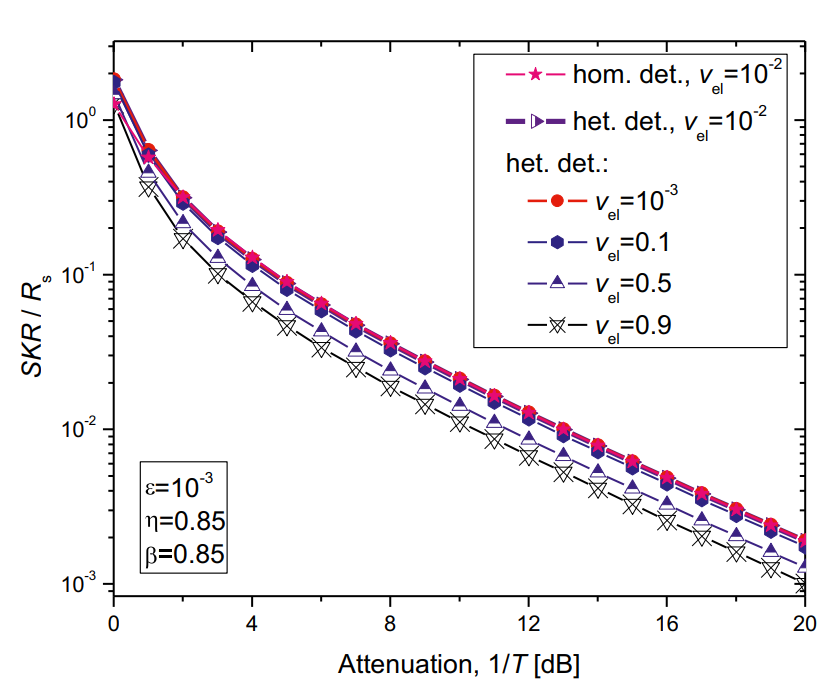
\includegraphics[width=0.7\textwidth]{chapters/figs/fig-6-28}
	\caption{کسر مخفی برای طرح توزیع کلید کوانتومی با متغیر پیوسته با مدولاسیون گاوسی برحسب تلفات کانال در شرایطی که واریانس نویز الکتریکی یک پارامتر است.}
	\label{fig:6-28}
\end{figure}

\begin{figure}[ht]
	\centering
	 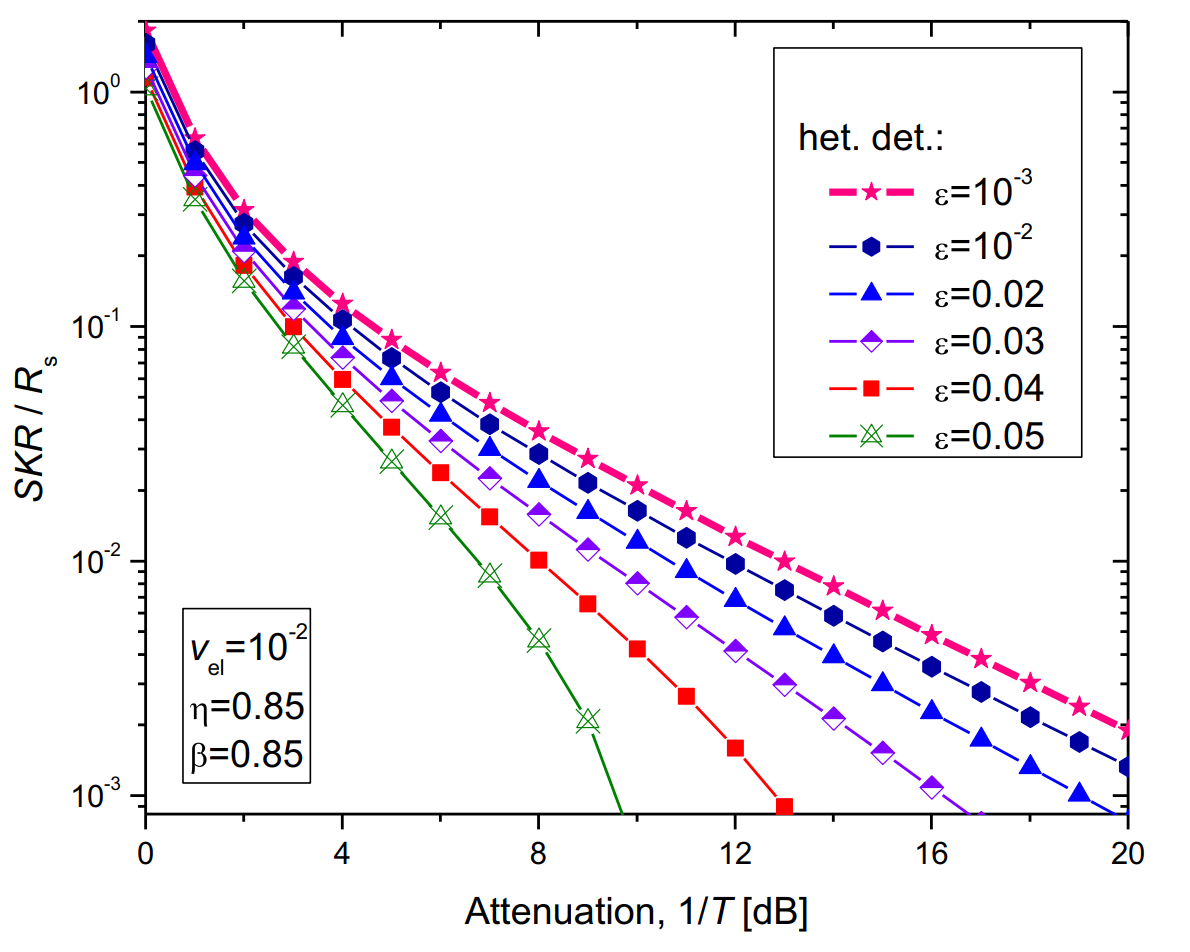
\includegraphics[width=0.7\textwidth]{chapters/figs/fig-6-29}
	\caption{کسر مخفی برای طرح توزیع کلید کوانتومی با متغیر پیوسته با مدولاسیون گاوسی برحسب تلفات کانال در شرایطی که واریانس نویز اضافی یک پارامتر است.}
	\label{fig:6-29}
\end{figure}

\begin{figure}[ht]
	\centering
	 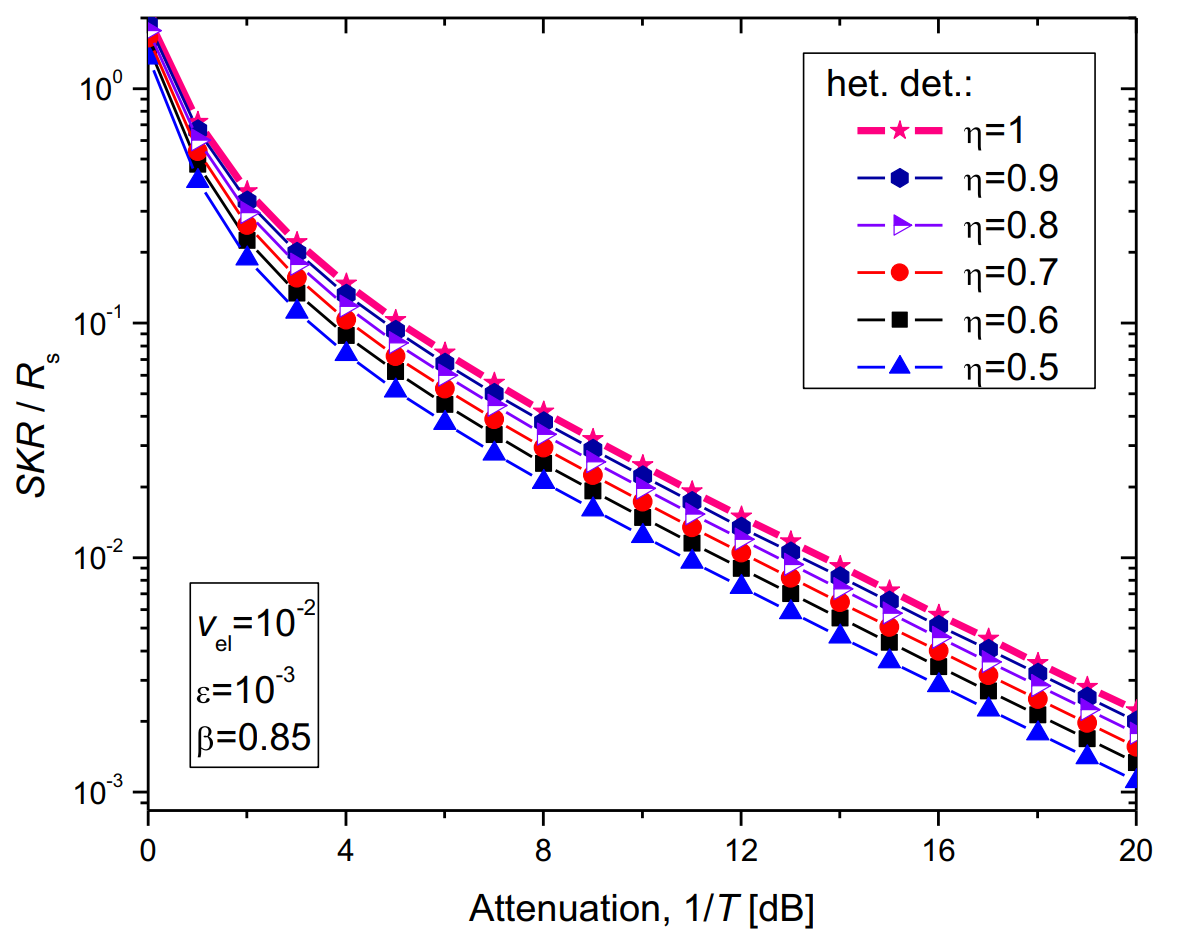
\includegraphics[width=0.7\textwidth]{chapters/figs/fig-6-30}
	\caption{کسر مخفی برای طرح توزیع کلید کوانتومی با متغیر پیوسته با مدولاسیون گاوسی برحسب تلفات کانال در شرایطی که بازدهی آشکارساز یک پارامتر است.}
	\label{fig:6-30}
\end{figure}

\section{خلاصه}
\label{sec:6-11}
این فصل به مفاهیم بنیادی \lr{QKD} اختصاص یافت. تفاوت‌های اصلی بین رمزنگاری متداول و \lr{QKD} در بخش \ref{sec:6-1} تشریح شد. در بخش مبانی \lr{QKD} (بخش \ref{sec:6-2})، پس از یک مرور تاریخی، انواع مختلف \lr{QKD} به‌اختصار معرفی شدند. بخش \ref{sec:6-3} به توصیف دو قضیه بنیادی پرداخت که \lr{QKD} بر آن‌ها استوار است؛ یعنی قضیه کپی‌ناپذیری و قضیه عدم توانایی در تمایز ابهام‌ناپذیر حالت‌های کوانتومی غیرمتعامد. در بخش \ref{sec:6-4}، مربوط به سیستم‌های \lr{DV-QKD}، پروتکل‌های \lr{BB84}، \lr{B92}، اکرت (\lr{E91})، \lr{EPR} و کدگذاری فاز-زمان در زیربخش‌های متناظر \ref{subsec:6-4-1} تا \ref{sec:6-4-4} شرح داده شدند. بخش \ref{sec:6-5} به امنیت \lr{QKD} اختصاص داشت که در آن \lr{SKR} به‌عنوان حاصل‌ضرب کلید خام و نرخ‌های کسری نمایش داده می‌شود. علاوه بر این، عبارت عمومی برای نرخ کسری ارائه شد و به‌دنبال آن استراتژی‌های مختلف شنود، از جمله حملات انفرادی (بخش \ref{subsec:6-5-1})، دسته‌جمعی (بخش \ref{subsec:6-5-2}) و حملات هک کوانتومی/کانال جانبی (بخش \ref{subsec:6-5-3}) توصیف شدند. برای حملات انفرادی و همدوس، عبارات کسر مخفی متناظر ارائه شد که شامل کسر مخفی برای پروتکل \lr{BB84} در بخش \ref{subsec:6-5-4} بود. در بخش \ref{sec:6-6}، پروتکل حالت فریب همراه با محاسبات \lr{SKR} مربوطه تشریح گردید.

\begin{figure}[ht]
	\centering
	 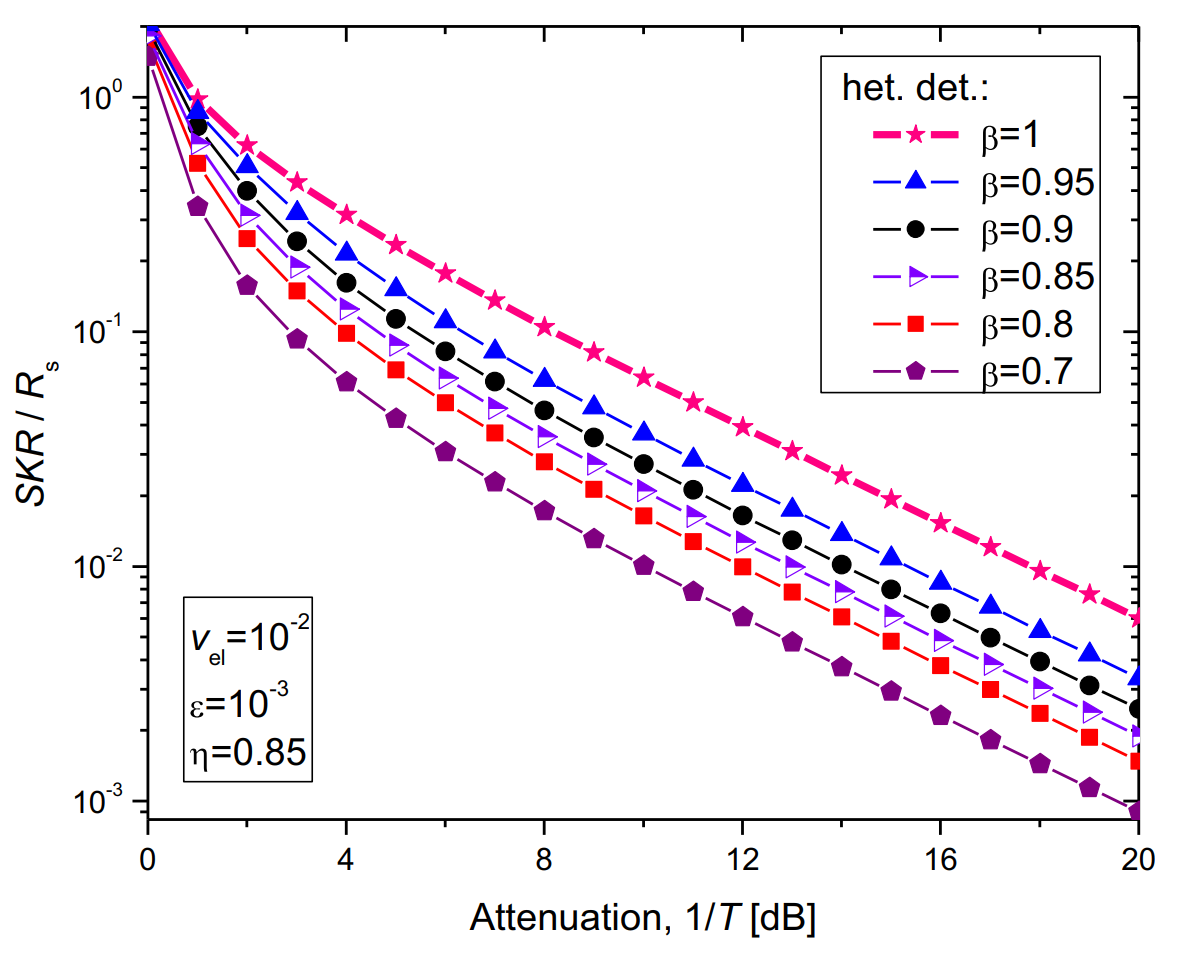
\includegraphics[width=0.7\textwidth]{chapters/figs/fig-6-31}
	\caption{کسر مخفی برای طرح توزیع کلید کوانتومی با متغیر پیوسته با مدولاسیون گاوسی برحسب تلفات کانال در شرایطی که بازدهی مصالحه یک پارامتر است.}
	\label{fig:6-31}
\end{figure}

مفاهیم کلیدی پروتکل \lr{MDI-QKD} در بخش \ref{sec:6-7} معرفی شدند که شامل \lr{BSM}های فوتونی (بخش \ref{subsec:6-7-1})، پروتکل \lr{MDI-QKD} مبتنی بر قطبش (بخش \ref{subsec:6-7-2}) و پروتکل \lr{MDI-QKD} مبتنی بر کدگذاری فاز-زمان (بخش \ref{subsec:6-7-3}) بود، در حالی که محاسبات کسر مخفی در بخش \ref{subsec:6-7-4} ارائه گردید. پروتکل‌های \lr{TF-QKD} در بخش \ref{sec:6-8} بیشتر تشریح شدند و عملکرد آن‌ها در برابر پروتکل‌های حالت فریب و \lr{MDI-QKD} ارزیابی شد. در بخش \ref{sec:6-9}، بحث به سمت مراحل پردازش کلاسیک، شامل گام‌های مصالحه اطلاعات (بخش \ref{sec:6-9-1}) و تقویت حریم خصوصی (بخش \ref{sec:6-9-2}) حرکت کرد.

بخش \ref{sec:6-10} به پروتکل‌های \lr{CV-QKD} اختصاص یافت که در آن طرح‌های آشکارسازی هموداین و هتروداین در بخش \ref{subsec:6-10-1}، پس از شرح مختصری از پروتکل‌های مبتنی بر حالت فشرده در بخش \ref{sec:6-10-2}، توصیف شدند. با توجه به اینکه تولید و دست‌کاری حالت‌های همدوس بسیار ساده‌تر است، پروتکل‌های مبتنی بر حالت همدوس به‌تفصیل در بخش \ref{subsec:6-10-3} شرح داده شدند. برای یک کانال ارسال با تلفات، ماتریس‌های کوواریانس متناظر برای طرح‌های آشکارسازی همدوس هموداین و هتروداین استخراج گردید و به‌دنبال آن، استخراج \lr{SKR} برای \lr{CV-QKD} مبتنی بر مدولاسیون گاوسی آماده‌سازی-و-اندازه‌گیری در بخش \ref{sec:6-10-4} انجام شد. برخی از نتایج مصالحه توصیفی در بخش \ref{sec:6-10-5} مربوط به طرح‌های \lr{CV-QKD} مبتنی بر مدولاسیون گاوسی ارائه گردید.


























